\documentclass[11pt,twoside]{book}
\usepackage[utf8]{inputenc}
\usepackage[spanish]{babel}
%%%%%%%%%%%%%%%%%%%%%%%%%%%%%%%%%%%%%%%%%%%%%%%%%%%%%%%%%%%%%%%%%%%%%%%%%%%%%%%%%%%%%%%%%%%%%%%%%%%%%%%
\usepackage{afterpage}% Necesario para introdicur páginas A3
\usepackage{amsmath,amsthm,amstext,amssymb}
\usepackage{capt-of}
\usepackage{colortbl}
\usepackage{graphicx}% Permite la introducción de figuras
\usepackage{array,fancyhdr,graphicx,subfigure,titlesec,titletoc,xcolor}
\usepackage{emptypage}% evita la numeración de las páginas en blanco
\usepackage{etoolbox}
\usepackage{listings} % premite la introducción de códigos vhdl
\usepackage[paper=A4,pagesize]{typearea}%necesario para introducir páginas A3
\usepackage{lscape}% Necesario para páginas apaisadas
\usepackage{pdfpages}% Permite introducir documentos pdf
\usepackage[font=small,bf]{caption}% Formato del caption
\usepackage{rotating}% Rotaciones
\usepackage{setspace,subfigure}
\usepackage{tocstyle}
\usepackage{codigomatlab}
\usepackage{titlesec}
\usepackage{color}
\usepackage{tikz}
\usetikzlibrary{calc}
\usepackage{pstricks}
\usepackage{pst-node}
\usepackage{pst-blur}
\usepackage{amsmath,amssymb}
\usepackage{booktabs}
\usepackage{xcolor}
\usepackage{colortbl}
\usepackage{rotating}
\usepackage{multirow}
\usepackage{bigstrut}
\usepackage{eurosym}
%\usepackage{inputenc}
%%%%%%%%%%%%%%%%%%%%%%%%%%%%%%%%%%%%%%%%%%%%%%%%%%%%%%%%%%%%%%%%%%%%%%%%%%%%%%%%%%%%%%%%%%%
\newcommand{\documento}{ÍÍNDICE XERAL}
%%%%%%%%%%%%%%%%%%%%%%%%%%%%%%%%%%%%%%%%%%%%%%%%%%%%%%%%%%%%%%%%%%%%%%%%%%%%%%%%%%%%%%%%%%%
% Incluye la bibliografía como sección
\makeatletter
\renewenvironment{thebibliography}[1]
     {\chapter{\bibname}% esta línea cambia la bibliografía a la categoría sección
      \@mkboth{\MakeUppercase\bibname}{\MakeUppercase\bibname}
      \list{\@biblabel{\@arabic\c@enumiv}}%
           {\settowidth\labelwidth{\@biblabel{#1}}
            \leftmargin\labelwidth
            \advance\leftmargin\labelsep
            \@openbib@code
            \usecounter{enumiv}
            \let\p@enumiv\@empty
            \renewcommand\theenumiv{\@arabic\c@enumiv}}
      \sloppy
      \clubpenalty4000
      \@clubpenalty \clubpenalty
      \widowpenalty4000%
      \sfcode`\.\@m}
     {\def\@noitemerr
       {\@latex@warning{Empty `thebibliography' environment}}
      \endlist}
\makeatother
%%%%%%%%%%%%%%%%%%%%%%%%%%%%%%%%%%%%%%%%%%%%%%%%%%%%%%%%%%%%%%%%%%%%%%%%%%%%%%%%%%%%%%%%%%%%%%%%%%%%%%%%%%%%%%%%%%%%%%%%%%%%%%%%%%%%%%%%%%%%%%%%%%%%%%%%%%%%%%%%%%%%%
%FORMATO DE LA HOJA
\renewcommand{\baselinestretch}{1.25}
\headsep 8mm        \topmargin -1.5cm     \textheight 24.5cm     \textwidth 16cm     \oddsidemargin 0.5cm     \evensidemargin -0.1cm
 \footnotesep=20pt               \footskip=38pt
%%%%%%%%%%%%%%%%%%%%%%%%%%%%%%%%%%%%%%%%%%%%%%%%%%%%%%%%%%%%%%%%%%%%%%%%%%%%%%%%%%%%%%%%%%%%%%%%%%%%%%%%%%%%%%%%%%%%%%%%%%%%%%%%%%%%%%%%%%%%%%%%%%%%%%%%%%%%%%%%%%%%%
% Formato del título de cada parte
\titleformat{\part}[display]
  {\normalfont\huge\bfseries}
	{}{0pt}{\centering}
	
\titlespacing*{\part}{0pt}{0pt}{20pt}
\titleclass{\part}{straight}
%%%%%%%%%%%%%%%%%%%%%%%%%%%%%%%%%%%%%%%%%%%%%%%%%%%%%%%%%%%%%%%%%%%%%%%%
%Formato del título de cada capítulo
\titleformat{\chapter}[hang] 
{\normalfont\huge\bfseries}{\thechapter}{1em}{} 
%%%%%%%%%%%%%%%%%%%%%%%%%%%%%%%%%%%%%%%%%%%%%%%%%%%%%%%%%%%%%%%%%%%%%%%%
% Espacio vertical en TOC
%\makeatletter
%\pretocmd{\part}{\addtocontents{toc}{\protect\addvspace{10\p@}}}{}{}
%\pretocmd{\chapter}{\addtocontents{toc}{\protect\addvspace{2\p@}}}{}{}
%\makeatother
%%%%%%%%%%%%%%%%%%%%%%%%%%%%%%%%%%%%%%%%%%%%%%%%%%%%%%%%%%%%%%%%%%%%%%
%Formato de letra
\usepackage{lmodern}
\renewcommand*\familydefault{\sfdefault} %% Only if the base font of the document 
%%%%%%%%%%%%%%%%%%%%%%%%%%%%%%%%%%%%%%%%%%%%%%%%%%%%%%%%%%%%%%%%%%%%%%%%%%%%%%%%%%%%%%%%%%%%
\renewcommand{\spanishtablename}{Tabla}% escribe Tabla
%\renewcommand*\listtablename{Índice de tablas}
%\renewcommand{\contentsname}{Contidos do PFG}
%%%%%%%%%%%%%%%%%%%%%%%%%%%%%%%%%%%%%%%%%%%%%%%%%%%%%%%%%%%%%%%%%%%%%%%%%%%%%%%%
\setcounter{secnumdepth}{5}% Profundidad del índice de contenidos
%%%%%%%%%%%%%%%%%%%%%%%%%%%%%%%%%%%%%%%%%%%%%%%%%%%%%%%%%%%%%%%%%%%%%%%%%%%%%%%%%%%%%%%%%%%%%%%%%%%%%%%%%%%%%%%%%%%%%%%%%%%%%%%%%%%%%%%%%%%%%%%%%%%%%%%%%%%%%%%%%%%%%%%%%%%%%
\numberwithin{equation}{subsection}
\usepackage{chngcntr}
\counterwithin{table}{subsection}% Numera las tablas por sucsecciones
\counterwithin{figure}{subsection}% Numera las figuras por sucsecciones

\DeclareCaptionLabelSeparator{guion}{\ --\ }
\captionsetup[figure]{labelsep=guion}% establece un guión como separador en el pie de figura
\captionsetup[table]{labelsep=guion}% establece un guión como separador en el pie de tabla
%%%%%%%%%%%%%%%%%%%%%%%%%%%%%%%%%%%%%%%%%%%%%%%%%%%%%%%%%%%%%%%%%%%%%%%%%%%%%%%%%%%%%%%%%%%%%%%%%%%%%%%%%%%%%%%%%%%%%%%%%%%%%%%%%%%
\usepackage{float}
\newfloat{Plano}{p}{pln}%[chapter]
\captionsetup[Plano]{labelformat=empty,labelsep=none,position=below}
%%%%%%%%%%%%%%%%%%%%%%%%%%%%%%%%%%%%%%%%%%%%%%%%%%%%%%%%%%%%%%%%%%%%%%%%%%%%%%%%%%%%%%%%%%%%%%%%%%%%%%%%%%%%%%%%%%%%%%%%%%%%%%%%%%%%%%%%%%%%%
\usepackage{float}
\newfloat{Circuito}{c}{cir}%[chapter]
\captionsetup[Circuito]{labelformat=empty,labelsep=none}
%%%%%%%%%%%%%%%%%%%%%%%%%%%%%%%%%%%%%%%%%%%%%%%%%%%%%%%%%%%%%%%%%%%%%%%%%%%%%%%%%%%%%%%%%%%%%%%%%%%%%%%%%%%%%%%%%%%%%%%%%%%%%%%%%%%%%%%%%%%%%
\usepackage[subfigure]{tocloft}% Permite cambiar el ancho de la numeración de listas de figuras y tablas
\addtolength{\cfttabnumwidth}{17pt}
\addtolength{\cftfignumwidth}{17pt}
\makeatletter
\let\l@lstlisting\l@figure
\makeatother
%%%%%%%%%%%%%%%%%%%%%%%%%%%%%%%%%%%%%%%%%%%%%%%%%%%%%%%%%%%%%%%%%%%%%%%%%%%%%%%%%%%%%%%%%%%%%%%%%%%%%%%%%%%%%%%%%%%%%%%%%%%%%%%%%%%%%%%%%%
\patchcmd{\chapter}{plain}{fancy}{}{}% Permite que el formato de la primera página sea como los demás
%%%%%%%%%%%%%%%%%%%%%%%%%%%%%%%%%%%%%%%%%%%%%%%%%%%%%%%%%%%%%%%%%%%%%%%%%%%%%%%%%%%%%%%%%%%%%%%%%%%%%%%%%%%%%%%%%%%%%%%%%%%%%%%%%%%%%%%%%%
\AtBeginDocument{\addtocontents{toc}{\protect\thispagestyle{fancy}}} % Permite que el formato de la página de tableofcontents sea como los demás
%%%%%%%%%%%%%%%%%%%%%%%%%%%%%%%%%%%%%%%%%%%%%%%%%%%%%%%%%%%%%%%%%%%%%%%%%%%%%%%%%%%%%%%%%%%%%%%%%%%%%%%%%%%%%%%
% Uso de las cabeceras fancy
\fancyhf{}
\fancyfoot[R]{\small \thepage}
\fancyfoot[C]{\small \raisebox{0pt}{\documento}}
\fancyhead[L]{\small \titulouno \ \\ \alumno}
% Introducir la especialidad-----------------------------------------------------------------------------------------------------
\fancyhead[C]{}% Escribir ELECTRICIDAD o ELECTRÓNICA                                                         -
% Introducir el número del PFG---------------------------------------------------------------------------------------------------
\fancyhead[R]{}% E es la especialidad 1=Electrónica 2=Electricidad   XXX es el número del proyecto     -
% Introducir la convocatoria del PFG---------------------------------------------------------------------------------------------
\fancyfoot[L]{}% Por ejemplo JUNIO 2014

\renewcommand{\headrulewidth}{0.5pt}
\renewcommand{\footrulewidth}{0.5pt}
%%%%%%%%%%%%%%%%%%%%%%%%%%%%%%%%%%%%%%%%%%%%%%%%%%%%%%%%%%%%%%%%%%%%%%%%%%%%%%%%%%%%%%%%%%%%%%%%%%%%%%%%%%%%%%%%%%%%%%%%%%%%%%%
% Paquete hyperref
\usepackage[colorlinks=true,linkcolor=red,citecolor=red,urlcolor=red]{hyperref}
%%%%%%%%%%%%%%%%%%%%%%%%%%%%%%%%%%%%%%%%%%%%%%%%%%%%%%%%%%%%%%%%%%%%%%%%%%%%%%%%%%%%%%%%%%%%%%%%%%%%
% Se cambio el nombre del caption para los códigos
\renewcommand\lstlistingname{Código}
%%%%%%%%%%%%%%%%%%%%%%%%%%%%%%%%%%%%%%%%%%%%%%%%%%%%%%%%%%%%%%%%%%%%%%%%%%%%%%%%%%%%%%%%%%%%%%%%%%%%%%%%%%%%%%%%%%%%%%%%%%%%%%%%%%
%  Permite meter figuras partidas en páginas
\newcommand\Image[3][]{
  \tabular[b]{@{}c@{}}\includegraphics[#1]{#2}\\
    {\small #3}
  \endtabular}
%%%%%%%%%%%%%%%%%%%%%%%%%%%%%%%%%%%%%%%%%%%%%%%%%%%%%%%%%%%%%%%%%%%%%%%%%%%%%%%%%%%%%%%%%%%%%%%%%%%%%%%%%%%%%%%%%%%%%%%%%%%%%%%%%%




%%%%%%%%%%%%%%%%%%%%%%%%%%%%%%%%%%%%%%%%%%%%%%%%%%%%%%%%%%%%%%%%%%%%%%%%%%%%%%%%%%%%%%%%%%%%%%%%%%%%%%%%%
%%%%%%%%%%%%%%%%%%%%%%%%%%%%%%%%%%%%%%%%%%%%%%%%%%%%%%%%%%%%%%%%%%%%%%%%%%%%%%%%%%%%%%%%%%%%%%%%%%%%%%%%%
%--------------------------------------------------------------------------------------------------------
%             Datos del ALUMNO
%--------------------------------------------------------------------------------------------------------
\newcommand{\alumno}{
% 1 Se debe introducir el NOMBRE y APELLIDOS del alumno (EN MAY�SCULAS)
Ávaro Fernádez Quesada
}
\newcommand{\especialidad}{
% 2 Introducir LA ESPECIALIDAD: ELECTR�NICA o ELECTRICA
Grao en Enxeñeríaren Electrónica Industrial e Automática
}
\newcommand{\grado}{
% 3 Introducir el grado: Electr�nica Industrial y Autom�tica o El�ctrica
Grao en Enxeñería en Electrónica Industrial e Automática
}
\newcommand{\materia}{
% 4 Introducir el nombre de la asignatura a la que se asocia el PFG
ASIGNATURA
}
%%%%%%%%%%%%%%%%%%%%%%%%%%%%%%%%%%%%%%%%%%%%%%%%%%%%%%%%%%%%%%%%%%%%%%%%%%%%%%%%%%%%%%%%%%%%%%%%%%%%%%%%%

%%%%%%%%%%%%%%%%%%%%%%%%%%%%%%%%%%%%%%%%%%%%%%%%%%%%%%%%%%%%%%%%%%%%%%%%%%%%%%%%%%%%%%%%%%%%%%%%%%%%%%%%%
%--------------------------------------------------------------------------------------------------------
%              Datos del PFG
%--------------------------------------------------------------------------------------------------------
% 5 Introducir EL T�TULO COMPLETO DEL PFG (EN MAY�SCULAS)
% El t�tulo suele ser largo y generalmente no cabe en una l�nea. La plantilla est� preparada para escribir el t�tulo en una, dos o tres l�neas. 
%------------------- BLOQUE: PRIMERA L�NEA DE T�TULO
\newcommand{\titulouno}{
Terminal de operador inalámbrico para preparación de pedidos dun almacén
}
%------------------- BLOQUE: S� HAY SEGUNDA L�NEA DE T�TULO
%-------------------
% Si existe segunda l�nea del t�tulo, activar (BORRAR %) este bloque y comentar (ESCRIBIR % AL PRINCIPIO DE CADA L�NEA) el siguiente. En la tercera l�nea de esta bloque se escribir� esa parte del t�tulo.
\newcommand{\titulodos}{
\colorbox{lightgray}{\large\bf 
 SEGUNDA L�NEA  DEL T�TULO
}}
%------------------- BLOQUE: NO HAY SEGUNDA L�NEA DE T�TULO
%-------------------
% Si no existe segunda l�nea del t�tulo, activar la siguiente l�nea y comentar el bloque anterior.
%\newcommand{\titulodos}{}
%
%------------------- BLOQUE: S� HAY TERCERA L�NEA DE T�TULO
%-------------------
% Si existe tercera l�nea del t�tulo, activar (BORRAR %) este bloque y comentar (ESCRIBIR % AL PRINCIPIO DE CADA L�NEA) el siguiente. 
% En la tercera l�nea de esta bloque se escribir� esa parte del t�tulo.
\newcommand{\titulotres}{
\colorbox{lightgray}{\large\bf 
TERCERA L�NEA  DEL T�TULO
}}
%------------------- BLOQUE: NO HAY TERCERA L�NEA DE T�TULO
%-------------------
% Si no existe tercera l�nea del t�tulo, activar la siguiente l�nea y comentar el bloque anterior.
%\newcommand{\titulotres}{}

%--------------------------------------------------------------------------------------------------
\newcommand{\numero}{
% 6 Introducir EL N�MERO DEL PFG (EN MAY�SCULAS)
770G0XAXX
}
%--------------------------------------------------------------------------------------------------
\newcommand{\convocatoria}{
% 7 Introducir LA CONVOCATORIA (EN MAY�SCULAS)
MES
}
%--------------------------------------------------------------------------------------------------
\newcommand{\anho}{
% 8 Introducir EL A�O
20XX
}
%--------------------------------------------------------------------------------------------------
\newcommand{\tutoruno}{
% 9 Introducir datos del tutor NOMBRE y APELLIDOS (EN MAY�SCULAS)
José Luis Camaño Portela
}
%------------------- BLOQUE: S� HAY SEGUNDO TUTOR
% Si hay segundo tutor, activar (BORRAR %) este bloque y comentar (ESCRIBIR % AL PRINCIPIO DE CADA L�NEA) el siguiente. En la tercera l�nea de esta bloque se escribir� esa parte del t�tulo.
\newcommand{\tutordos}{
\colorbox{lightgray}{\large\bf 
NOMBRE APELLIDO1 APELLIDO2
}}
%------------------- BLOQUE: NO HAY SEGUNDO TUTOR
%-------------------
% Si no hay segundo tutor, activar la siguiente l�nea y comentar el bloque anterior.
%\newcommand{\tutordos}{}
%%%%%%%%%%%%%%%%%%%%%%%%%%%%%%%%%%%%%%%%%%%%%%%%%%%%%%%%%%%%%%%%%%%%%%%%%%%%%%%%%%%%%%%%%%%%%%%%%%%%%%%%%
%%%%%%%%%%%%%%%%%%%%%%%%%%%%%%%%%%%%%%%%%%%%%%%%%%%%%%%%%%%%%%%%%%%%%%%%%%%%%%%%%%%%%%%%%%%%%%%%%%%%%%%%%







%\renewcommand\lstlistlistingname{Lista de códigos Arduino} 
%		\renewcommand\lstlistingname{Código}
		
		\definecolor{mygray}{rgb}{0.47,0.47,0.33}
\definecolor{myorange}{rgb}{0.8,0.4,0}
\definecolor{myblue}{rgb}{0,0.4,0.7}



\lstset{ %
  %backgroundcolor=\color{mywhite},  
	language=C,
  basicstyle=\footnotesize,       
  breakatwhitespace=false,         
  breaklines=true,                 
  captionpos=t, 
	belowcaptionskip=0.8cm,
  commentstyle=\color{mygray},
	deletekeywords={...},           
  escapeinside={\%*}{*)},          
  extendedchars=true,              
  frame=single,                    
  keepspaces=true,                 
  %keywordstyle=\color{myorange},
	morekeywords=[1]{delay,digitalWrite,loop,setup},
	morekeywords=[2]{HIGH,LOW,OUTPUT},
  keywordstyle = [1]\color{myorange}\bfseries,
	keywordstyle = [2]\color{myblue}\bfseries,
  numbers=left,                    
  numbersep=5pt,                   
  numberstyle=\tiny\color{mygray}, 
  rulecolor=\color{black},         
  %rulesepcolor=\color{myblue},
  showspaces=false,                
  showstringspaces=false,          
  showtabs=false,                  
  stepnumber=1,                    
  stringstyle=\color{myorange},    
  tabsize=2,                       
  title=\lstname                   
}   
% Opciones: vhdl, arduino
%%%%%%%%%%%%%%%%%%%%%%%%%%%%%%%%%%%%%%%%%%%%%%%%%%%%%%%%%%%%%%%%%%%%%%%%%%%%%%%%%%%%%%%%%%%%%%%%%%%%%%%%%%%%%%%%%
\begin{document}
% Se incluye la portada del TFG
\pagestyle{empty}

\begin{tikzpicture}[remember picture, overlay]
  \draw[line width = 0.5pt] ($(current page.north west) + (86pt,-43.5pt)$) rectangle ($(current page.south east) + (-46.5pt,43.5pt)$);
\end{tikzpicture}

\begin{center}
\begin{figure}[htbp]
\begin{center}

\includegraphics[angle=0, height=3.8cm]{images/EEILogo.png}
\end{center}
\end{figure}
\ \\
\begin{large}
\begin{center}
\color{blue}\textbf{Escola de Enxeñería Industrial}
\end{center}
\end{large}
\ \\
\ \\
\begin{large}
\begin{center}
\textbf{TRABALLO FIN DE GRAO}
\end{center}
\end{large}
\ \\
\ \\
\begin{large}
\begin{center}
{\titulouno}
\end{center}
\end{large}
\ \\
\ \\
\begin{normalsize}
\begin{center}
\textbf{\grado}
\end{center}
\end{normalsize}
\ \\
\ \\
\ \\
\ \\
\begin{normalsize}
\begin{center}
\textbf{Alumno:  \qquad \qquad \alumno}
\end{center}
\end{normalsize}
\ \\
\begin{normalsize}
\begin{center}
\textbf{Directores: \qquad \qquad \tutoruno}
\end{center}
\end{normalsize}
\ \\
\ \\
\ \\
\ \\

\begin{center}
\begin{figure}[htbp]
\begin{center}

\includegraphics[angle=0, height=0.8cm]{images/UVIGOLogo.png}
\end{center}
\end{figure}
\end{center}

\end{center}


\cleardoublepage
%%%%%%%%%%%%%%%%%%%%%%%%%%%%%%%%%%
% Página de resumen del proyecto %
%%%%%%%%%%%%%%%%%%%%%%%%%%%%%%%%%%

\thispagestyle{empty}

\bigskip
\bigskip

\large{
\textbf{Resumo:}}

\bigskip
\bigskip


\begin{center}
\textbf{\titulouno}
\end{center}

\bigskip
\bigskip
%\bigskip
\large{
\textbf{Alumno:}}\alumno

%\medskip
\large{
\textbf{Director:}} \tutoruno

%\vfill

%\begin{minipage}{\textwidth}
%\textbf{Dpto. de:}
%


%\medskip
%
%\textbf{Titulación:} Ingeniería de Telecomunicación
%
%\medskip
\bigskip
\bigskip


O presente proxecto lévase a cabo a implementación de un sistema de xestión de preparación de pedidos de varios productos nun almacén.

Desarrollouse un programa elaborado en C++ para unha placa Arduino para que sirva como terminal de operador para un carretilleiro de un almacén e que desde o cal podan xestionar encargos comunicándose por WiFi a un servidor.

O terminal de operador está composto por unha pantalla LCD para visualizar en todo momento o encargo e por un teclado matricial para indicar que o producto depositouse nunha caixa.
A comunicación por WiFi é levada a cabo polo módulo ESP8266 mediante servicios REST a un servidor que dispón dunha base de datos relacional.

O entorno de desenvolvemento dos servicios REST fixéronse con un framework de python chamado API RESTful Django e o programa para Arduino, por Atom.
 

\bigskip
\bigskip

\textbf{Palabras clave:} IoT, Picking, Almacén, Arduino, Servicios RESTful, Python.

%\begin{center} Vigo, \today\end{center}
%\end{minipage}

%Página en blanco
\newpage{\pagestyle{empty}\cleardoublepage}
\cleardoublepage
%%%%%%%%%%%%%%%%%%%%%%%%%%%%%%%%%%%%%%%%%%%%%%%%%%%%%%%%%%%%%%%%%%%%%%%%%%%%%%%%%%%%%%%%%%%%%%%%%%%%%%%%%%%%%%%%%%
% DOCUMENTO ÍNDICE XERAL
\pagestyle{empty}

\begin{tikzpicture}[remember picture, overlay]
  \draw[line width = 0.5pt] ($(current page.north west) + (-20pt,-800.5pt)$) rectangle ($(current page.south east) + (-133.5pt,-722.5pt)$);
\end{tikzpicture}

\renewcommand{\document}{ÍNDICE XERAL}

\begin{center}
\begin{figure}[htbp]
\begin{center}

\includegraphics[angle=0, height=3.8cm]{images/EEILogo.png}
\end{center}
\end{figure}
\ \\
\begin{large}
\begin{center}
\color{blue}\textbf{Escola de Enxeñería Industrial}
\end{center}
\end{large}
\ \\
\ \\
\begin{large}
\begin{center}
\textbf{TRABALLO FIN DE GRAO}
\end{center}
\end{large}
\ \\
\ \\
\begin{large}
\begin{center}
{\titulouno}
\end{center}
\end{large}
\ \\
\ \\
\begin{normalsize}
\begin{center}
\textbf{\grado}
\end{center}
\end{normalsize}
\ \\
\ \\
\ \\
\ \\
\begin{normalsize}
\begin{center}
\textbf{Documento}
\end{center}
\end{normalsize}
\ \\
\begin{normalsize}
\begin{center}
\part{\bf{ÍNDICE XERAL}}\thispagestyle{empty}
\end{center}
\end{normalsize}
\ \\
\ \\
\ \\
\ \\

\begin{center}
\begin{figure}[htbp]
\begin{center}

\includegraphics[angle=0, height=0.8cm]{images/UVIGOLogo.png}
\end{center}
\end{figure}
\end{center}

\end{center}



%%%%%%%%%%%%%%%%%%%%%%%%%%%%%%%%%%%%%%%%%%%%%%%%%%%%%%%%%%%%%%%%%%%%%%%%%%%%%%%%%%%%%%%%%%%%%%%%%%%%%%%%%%%%%%%%%%
\cleardoublepage



% Página que contiene el Índice de contenidos del TFG
\renewcommand{\contentsname}{Contido do TFG}
\addcontentsline{toc}{section}{Contidos do TFG}
%\setcounter{tocdepth}{3}
{\hypersetup{hidelinks}\tableofcontents}
\addtocontents{toc}{\protect\thispagestyle{fancy}}

% Página que contiene el Índice de listas de figuras
\cleardoublepage
\phantomsection
\renewcommand*\listfigurename{Índice de figuras}
\addcontentsline{toc}{section}{\listfigurename}
{\hypersetup{hidelinks}\listoffigures}
\addtocontents{lof}{\protect\thispagestyle{fancy}}

% Página que contiene el índice de listas de tablas
\cleardoublepage
\phantomsection
\renewcommand*\listtablename{Índice de tablas}
\addcontentsline{toc}{section}{\listtablename}
{\hypersetup{hidelinks}\listoftables}
\addtocontents{lot}{\protect\thispagestyle{fancy}}

\cleardoublepage

%%%%%%%%%%%%%%%%%%%%%%%%%%%%%%%%%%%%%%%%%%%%%%%%%%%%%%%%%%%%%%%%%%%%%%%%%%%%%%%%%%%%%%%%%%%%%%%%%%%%%%%%%%%%%
%%%%%%%%%%%%%%%%%%%%%%%%%%%%%%%%%%%%%%%%%%%%%%%%%%%%%%%%%%%%%%%%%%%%%%%%%%%%%%%%%%%%%%%%%%%%%%%%%%%%%%%%%%%%%
% DOCUMENTO MEMORIA
\pagestyle{empty}

\begin{tikzpicture}[remember picture, overlay]
  \draw[line width = 0.5pt] ($(current page.north west) + (-20pt,-800.5pt)$) rectangle ($(current page.south east) + (-133.5pt,-722.5pt)$);
\end{tikzpicture}

\renewcommand{\documento}{MEMORIA}

\begin{center}
\begin{figure}[htbp]
\begin{center}

\includegraphics[angle=0, height=3.8cm]{images/EEILogo.png}
\end{center}
\end{figure}
\ \\
\begin{large}
\begin{center}
\color{blue}\textbf{Escola de Enxeñería Industrial}
\end{center}
\end{large}
\ \\
\ \\
\begin{large}
\begin{center}
\textbf{TRABALLO FIN DE GRAO}
\end{center}
\end{large}
\ \\
\ \\
\begin{large}
\begin{center}
{\titulouno}
\end{center}
\end{large}
\ \\
\ \\
\begin{normalsize}
\begin{center}
\textbf{\grado}
\end{center}
\end{normalsize}
\ \\
\ \\
\ \\
\ \\
\begin{normalsize}
\begin{center}
\textbf{Documento}
\end{center}
\end{normalsize}
\ \\
\begin{normalsize}
\begin{center}
\part{\bf{MEMORIA}}
\end{center}
\end{normalsize}
\ \\
\ \\
\ \\
\ \\

\begin{center}
\begin{figure}[htbp]
\begin{center}

\includegraphics[angle=0, height=0.8cm]{images/UVIGOLogo.png}
\end{center}
\end{figure}
\end{center}

\end{center}

\cleardoublepage


\pagestyle{fancy}
%%%%%%%%%%%%%%%%%%%%%%%%%%%%%%%%%%%%%%%%%%%%%%%%%%%%%%%%%%%%%%%%%%%%%%%%%%%%%%%%%%%%%%%%%%%%%%%%%%%%%%%%%%%%%%
%%%%%%%%%%%%%%%%%%%%%%%%%%%%%%%%%%%%%%%%%%%%%%%%%%%%%%%%%%%%%%%%%%%%%%%%%%%%%%%%%%%%%%%%%%%%%%%%%%%%%%%%%%%%%

\addcontentsline{toc}{section}{Índice do documento Memoria}
\startcontents[parts]
\begin{center}{\large \bf Índice de MEMORIA}\end{center}

{\hypersetup{hidelinks}\printcontents[parts]{}{-1}{\setcounter{tocdepth}{5}}}

\cleardoublepage%----------------------------------------

\chapter{Introducción}

\section{Estado de arte}

Hoxe en día todo está conectado á rede, non so persoas conectadas a través de un dispositivo, senón a calqueira``cousa'' que teña algunha funcionalidade e que poida ser controlado dende calqueira dispositivo, xa sexa desde un smartphone, un ordenador ou dende un smartwatch. Esto é debido á implementación de IoT (Internet of Things). Pódese definir como \textit{<<unha rede que conecta ``cousas'' identificables de maneira única a Internet. As ``cousas'' teñen capacidades de captura/actuación e de potencial de programación. Mediante a explotación  da identificación e captura única, pódese recoller información mais cambiar o estado da ``cousa'' onde queiras, en calquer momento e por calquera motivo>>} \cite{IoT}

\begin{figure}[H]
	\begin{center}
		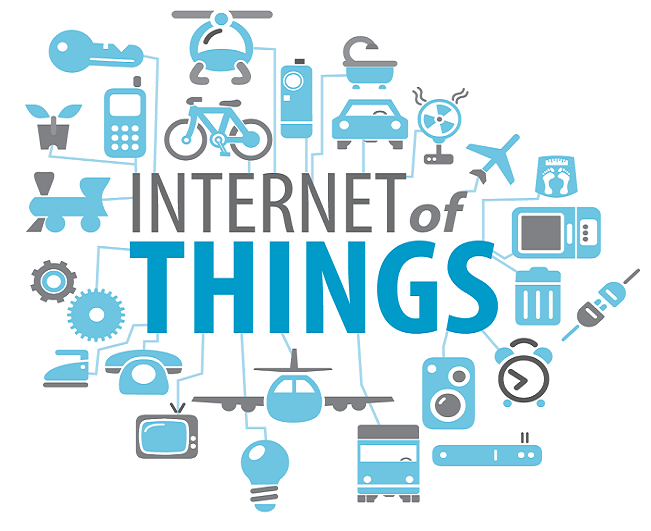
\includegraphics[width=10cm]{images/IoT.png}
	\end{center}
	\caption{Internet of Things *http://www.pcworldenespanol.com/}
	\label{fig:IoT}
\end{figure}

\section{Obxecto}

O obxectivo principal do proxecto vai ser o de realizar a monitorización de un procesado de un pedido ou picking nun almacén para un operario a través dun terminal de operador inalámbrico.

\begin{figure}[H]
	\begin{center}
		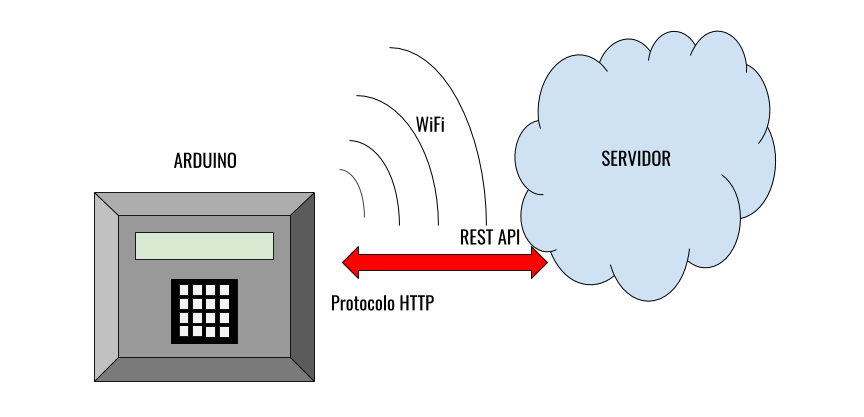
\includegraphics[width=10cm]{images/esquema_xeral.png}
	\end{center}
	\caption{Esquema xeral do proxecto}
	\label{fig:IoT}
\end{figure}

Debido ós altos costes dos terminales, como por exemplo SYMBOL VC5090, pensouse en realizalo cunha placa Arduino e o módulo WiFi ESP8266 pola súa capacidade de programación e, por suposto, polo seu prezo.
Por outro lado, tamén conta cunha interfaz web para o almacén, podendo xestionar tanto os productos coma os pedidos.

\begin{figure}[H]
	\begin{center}
		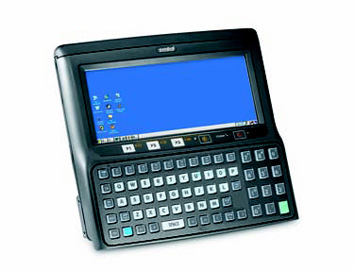
\includegraphics[width=10cm]{images/symbol_VC5090.jpg}
	\end{center}
	\caption{Terminal de operador SYMBOL VC5090 *http://www.datanet.com.au/}
	\label{fig:IoT}
\end{figure}

Para elo, vaise dividir o documento \textbf{Memoria} en compoñentes hardware, onde se vai detallar todos os elementos usados (Arduino e módulos), e compoñentes software, onde se explicará a parte de programación da parte de \txtbf{Arduino} e a parte de \textbf{Django RESTful Service}.

\chapter{Conceptos previos}

\section{Preparación de pedidos ou picking}

No mundo da loxística, realizar picking de un producto consiste en ir a unha estantería ou zona concreta dentro do almacén para recoller os productos requeridos para un pedido. É un proceso importante dentro empresas tanto pequenas coma grades, polo que é importante a súa optimización e mecanización.

\subsection{Formas de preparación de pedido}
Dentro picking, existen infinitas metodoloxías tradicionais de xestionalo, que veñen determinadas pola tipoloxía do almacén, niveis de servicios que da a empresa, etc. 
Pódense clasificar segundo:

\begin{itemize}
    \item Onde o efectuamos
        \begin{itemize}
            \item \textbf{De home a pedido:} Os operarios recorren o almacén e seleccionar o producto. 
            \item \textbf{De producto a home:} O producto é o que se desplaza ata o posto no que está o operario. Ten unha maior inversión económica pero reduce o tempo.
        \end{itemize}
    \item Como extraemos a mercancía
        \begin{itemize}
            \item \textbf{Pedido a pedido: } Os operarios preparan de forma individual os pedidos, é decir, solo preparan un pedido á vez. 
            \item \textbf{Por oleaxe: } Realizan picking de varios pedidos á vez. Merece a pena se hai poucos pedidos e moita repetividade. 
        \end{itemize}
    \item A unidade de extracción
        \begin{itemize}
            \item \textbf{De caixas completas.}
            \item \textbf{De unidades soltas.}
        \end{itemize}
\end{itemize}

En concreto neste proxecto, a metodoloxía vai ser picking de home a producto, de pedido a pedido e de unidades soltas.

\section{Arduino}
\subsection{Historia}

Arduino nace polo ano 2005 como un proxecto de estudiantes no Instituto de Diseño Interactivo Ivrea de Italia (IDII), onde os alumnos experimentaban con distintos tipos de microcontroladores. A idea era crear unha ferramenta moderna, sencilla, barata e fácil de usar. Foi así como empezaron a desenvolvela baixo a licencia de Open Source, para que todo o mundo poidese contribuir. \cite{wArduino}

\subsection{Placas}

Hai moitas variedades de placas. Na táboa de abaixo móstranse as características das principais:

\begin{table}[htb]
\begin{center}
\resizebox{16cm}{!} {
\begin{tabular}{|c|m{3cm}|m{3.5cm}|m{2cm}|m{2cm}|m{2cm}|m{2cm}|m{2cm}|m{2cm}|c|c|}
\hline
Nombre & Procesador & Operating/Voltage Input & CPU Speed & Analogic In/Out & Digital IO/PWM & EEPROM & SRAM & FLASH & USB & UART \\
\hline
101 & Intel Curie & 3.3V/7-12V & 32MHz & 6/0 & 14/4 & - & 24 & 196 & Regular & - \\ 
\hline
Gemma & ATtiny85 & 3.3 V / 4-16 V & 8 MHz & 1/0 & 3/2 & 0.5 & 0.5 & 8 & Micro & 0 \\
\hline
LilyPad & ATmega168V \newline ATmega328P & 2.7-5.5 V/2.7-5.5 V & 8MHz & 6/0 & 14/6 & 0.512 & 1 & 16 & - & - \\
\hline
LilyPad SimpleSnap & ATmega328P & 2.7-5.5 V/2.7-5.5 V & 8 MHz & 4/0 & 9/4 & 1 & 2 & 32 & - & - \\
\hline
LilyPad USB & ATmega32U4 & 3.3 V/3.8-5 V & 8 MHz & 4/0 & 9/4 & 1 & 2.5 & 32 & Micro & - \\
\hline
Mega 2560 & ATmega2560 & 5V/7-12 V & 16 MHz & 16/0 & 54/15 & 4 & 8 & 256 & Regular & 4 \\
\hline
Micro & ATmega32U4 & 5 V/7-12 V & 16 MHz & 12/0 & 20/7 & 1 & 2.5 & 32 & Micro & 1 \\
\hline
MKR1000 & SAMD21 Cortex-M0+ & 3.3 V/ 5V  & 48MHz  & 7/1 & 8/4 & - & 32 & 256 & Micro & 1 \\
\hline
Pro & ATmega168 ATmega328P & 3.3 V/3.35-12 V \newline  5 V/5-12 V & 8 MHz  \newline  16 MHz & 6/0 & 14/6 & 0.512 \newline 1 & 1   2 & 16  32 & - & 1 \\
\hline
Pro Mini & ATmega328P & 3.3 V / 3.35-12 V \newline  5 V / 5-12 V & 8 MHz \newline  16 MHz & 6/0 & 14/6 & 1 & 2 & 32 & - & 1 \\
\hline
Uno & ATmega328P & 5 V / 7-12 V & 16 MHz & 6/0 & 14/6 & 1 & 2 & 32 & Regular & 1 \\
\hline
Zero & ATSAMD21G18 & 3.3 V / 7-12 V & 48 MHz & 6/1 & 14/10 & - & 32 & 256 & 2 Micro & 2 \\
\hline
Due & ATSAM3X8E & 3.3 V / 7-12 V & 84 MHz & 12/2 & 54/12 & - & 96 & 512 & 2 Micro & 4\\
\hline
Esplora & ATmega32U4 & 5 V / 7-12 V & 16 MHz & - & - & 1 & 2.5 & 32 & Micro & - \\
\hline
Ethernet & ATmega328P & 5 V / 7-12 V & 16 MHz & 6/0 & 14/4 & 1 & 2 & 32 & Regular & - \\
\hline
Leonardo & ATmega32U4 & 5 V / 7-12 V & 16 MHz & 12/0 & 20/7 & 1 & 2.5 & 32 & Micro & 1 \\
\hline
Mega ADK & ATmega2560 & 5 V / 7-12 V & 16 MHz & 16/0 & 54/15 & 4 & 8 & 256 & Regular & 4 \\
\hline
Mini & ATmega328P & 5 V / 7-9 V & 16 MHz & 8/0 & 14/6 & 1 & 2 & 32 & - & - \\
\hline
Nano & ATmega168 \newline ATmega328P & 5 V / 7-9 V & 16 MHz & 8/0 & 14/6 & 0.512  1 & 1  2 & 16 32 & Mini & 1 \\
\hline
Yún & ATmega32U4 \newline AR9331 Linux & 5 V & 16 MHz \newline 400MHz & 12/0 & 20/7 & 1 & 2.5 \newline  16MB & 32 \newline   64MB & Micro & 1 \\
\hline
Arduino Robot & ATmega32u4 & 5 V & 16 MHz & 6/0 & 20/6 & 1 KB (ATmega32u4)/512 Kbit (I2C) & 2.5 KB (ATmega32u4) & 32 KB (ATmega32u4) of which 4 KB used by bootloader & 1 & 1 \\
\hline
MKRZero & SAMD21 \newline  Cortex-M0+32bit low power \newline ARM MCU & 3.3 V & 48 MHz & 7 (ADC 8/10/12 bit)/1 (DAC 10 bit) & 22/12 & No & 32 KB & 256 KB & 1 & 1 \\
\hline
\end{tabular}
}
\caption{Comparación de placas Arduino}
\label{taboa:comparacionPlacasArduino}
\end{center}
\end{table}

Neste proxecto vaise usar Arduino Mega 2560.

\subsection{Entorno de Programación}

O entorno de desenvolvemento integrado (Integrated Development Environment ou IDE) é un programa informático composto por un conxunto de ferramentas de programación. 

Arduino ten un IDE propio chamado Arduino IDE, pero por comodidade vaise empregar Atom cun plugin chamado \textit{PlatformIO}, que vai permitir poder compilar, subir e depurar código na placa.

\begin{figure}[H]
	\begin{center}
		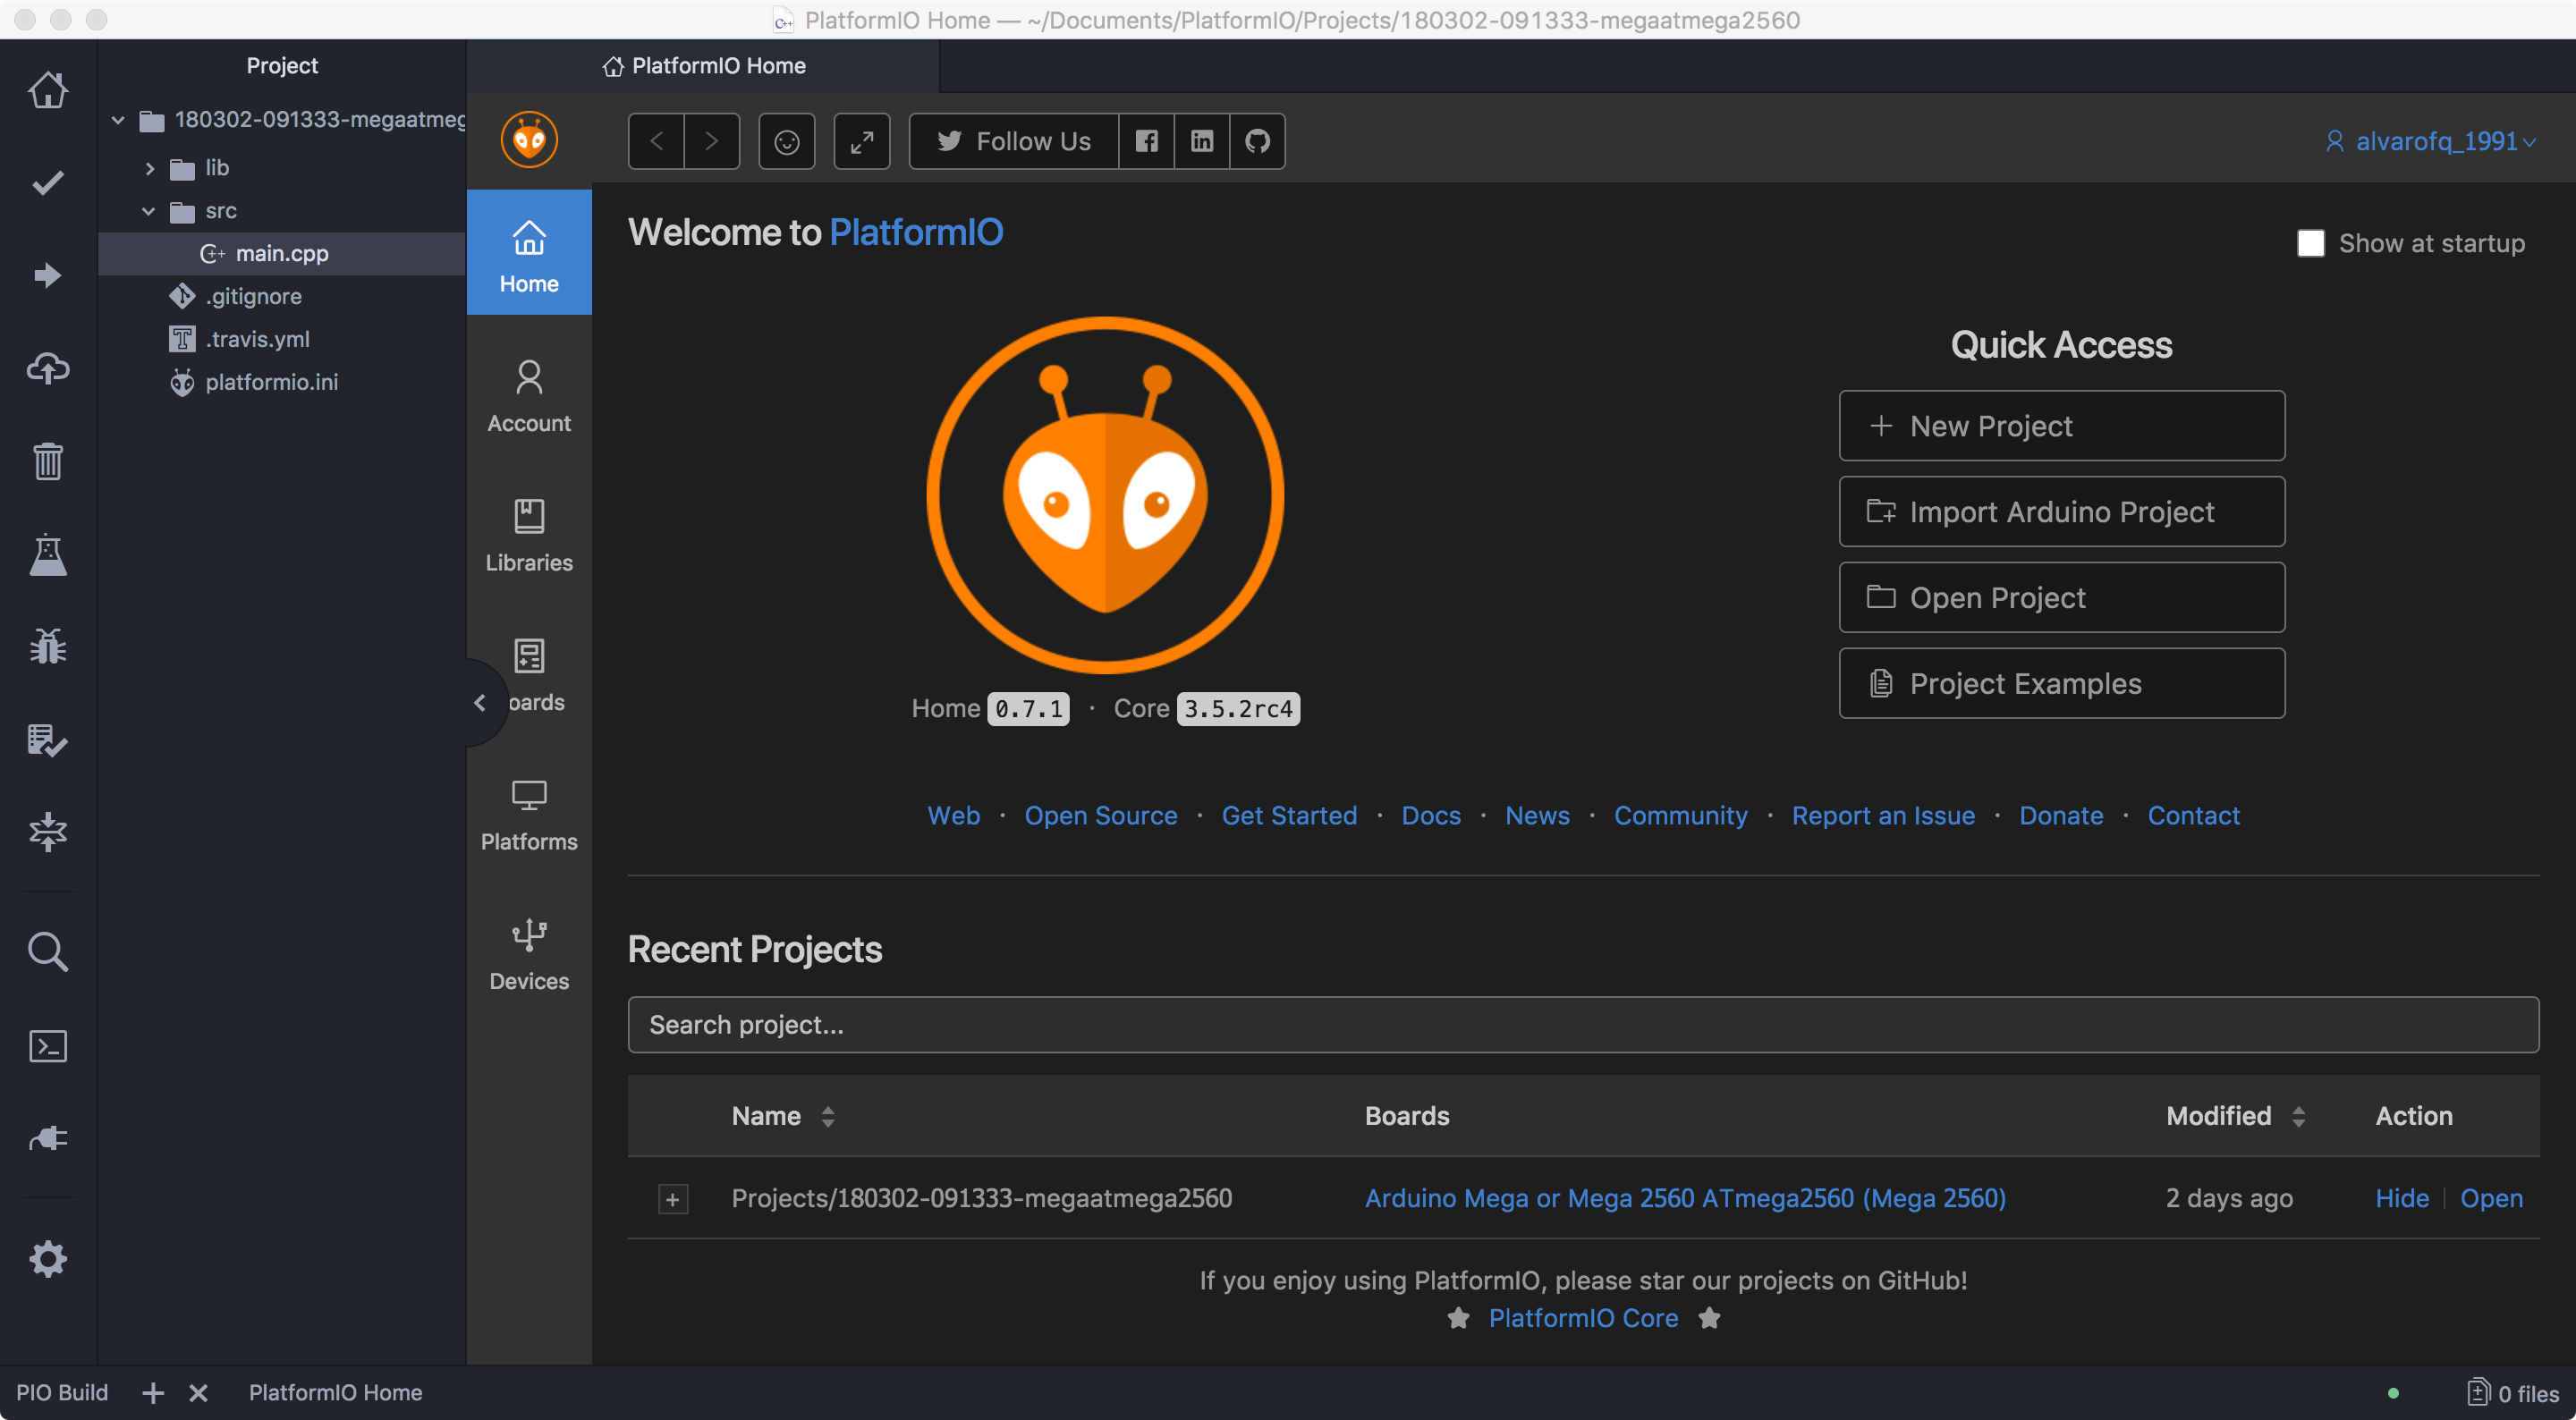
\includegraphics[width=15cm]{images/Atom.png}
	\end{center}
	\caption{Atom}
	\label{fig:Atom}
\end{figure}

Para a creación dun novo proxecto, faise click en New Project, poñéndolle un nome e seleccionando a placa usada, que neste caso vai ser Arduino Mega 2560.

\begin{figure}[H]
	\begin{center}
		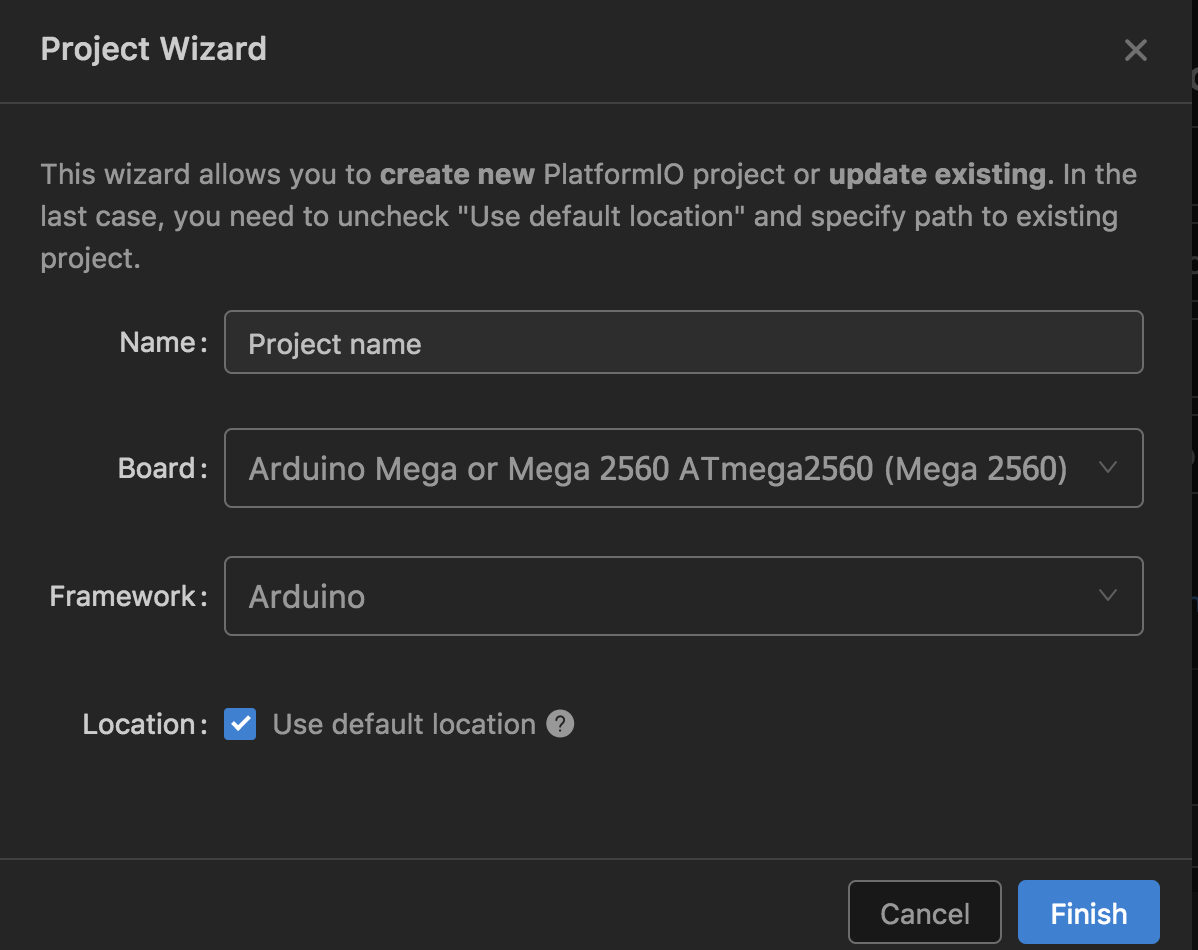
\includegraphics[width=8cm]{images/NewProject.png}
	\end{center}
	\caption{Novo Proxecto}
	\label{fig:NewProject}
\end{figure}

\subsection{Sketches}

Os programas de Arduino, tamén chamados Sketch, están compostos por un solo ficheiro con extensión ``.ino'', pero neste caso, o arquivo vai ter extensión ``.cpp'' como no lenguaxe de programación C++.

\subsection{Librerías}

Na aplicación, pódese incorporar librerías codificadas por outros programadores. Esto facilita á hora de programar e permite a abstracción facendo que o noso programa sexa moito máis fácil de elaborar e entender.

Disponse de infinidade de librerías para facilitar traballo, sendo todas elas Open Source.

Normalmente veñen comprimidas nun archivo ZIP e conteñen:
\begin{itemize}
\item Un archivo .cpp (código C++)
\item Un arquivo de declaracións con extensión .h que contén a declaración dunha ou varias clases.
\item Un directorio con varios exemplos para axudarnos a entendela.
\end{itemize}

Para incluir librerías no noso proxecto, na carpeta chamada ``lib'' importaranse, creando un packete para cada unha.

\begin{figure}[H]
	\begin{center}
		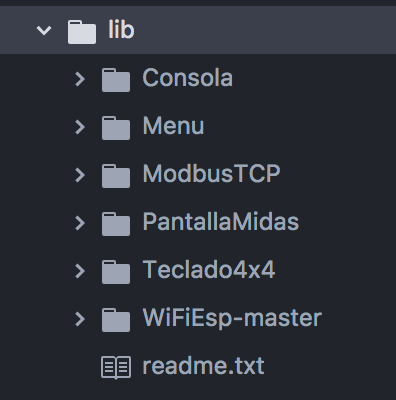
\includegraphics[width=7cm]{images/librerias.png}
	\end{center}
	\caption{Incluir librerías}
	\label{fig:LibreriasAtom}
\end{figure}

\subsection{Serial Monitor}

PlatformIO ten tamén a opción mostrar o que se comunique ca placa Arduino por medio do porto Serial.
Esto vai ser útil á hora do desenvolvemento, xa que permite imprimir por pantalla datos ou estadísticas.
 Para eso, vaise o apartado Serial Monitor e configuraremos o porto no que temos conectada a placa e os ``baudios'', que é a velocidade de retransmision.
 
 \begin{figure}[H]
	\begin{center}
		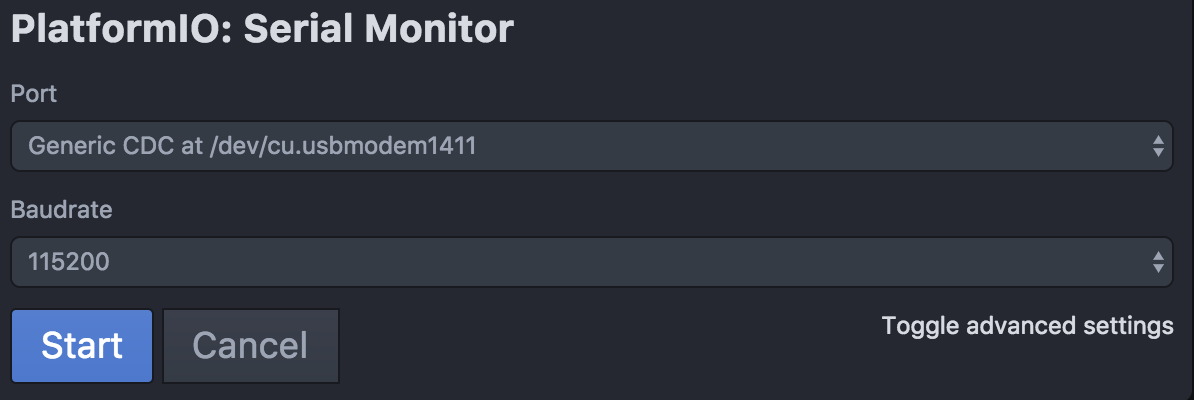
\includegraphics[width=7cm]{images/serial_monitor.png}
	\end{center}
	\caption{Serial Monitor}
	\label{fig:LibreriasAtom}
\end{figure}

\section{API REST}

API (Application Programming Incerface) é unha colección de funcións e métodos desenvolvidas para dotar dunha capa de abstracción para o manexo dun dispositivo, estructura de datos ou calqueira outra funcionalidade. 

REST (Representational State Transfer) é unha arquitectura de desenvolvemento web que usa o estándar HTTP.

\subsection{Arquitectura}

\subsubsection{Identificación de recursos con URI's}

Un recurso representa unha sección, arquivo ou contido que queremos obter ou modificar. Para poder identificalo, usaremos URI's, que teñen que cumprir:
\begin{itemize}
    \item Non se debe usar verbos nos nomes de URI.
    \item Deben ser únicas.
    \item Non deben tomar en conta o formato.
    \item Deben ter unha xerarquía lóxica.
    \item Os filtrados de información faranse mediante parámetros HTTP.
    \item Debe usarse a súa forma plural.
\end{itemize}

\subsubsection{Métodos HTTP}

Os principais métodos son:

\begin{itemize}
    \item GET: Consulta e lectura de recursos.
    \item POST: Creación de recursos.
    \item PUT: Edición de recursos.
    \item DELETE: Eliminación de recursos.
    \item PATCH: Edicion de partes de recursos.
\end{itemize}

\section{Django}

Django é un framework Open Source para o desenvolvemento de aplicacións web. Está escrito na lenguaxe \textbf{Python}. Contén un conxunto de compoñentes que van axudar a compoñer aplicacións web facil e rapidamente.

Para usar unha estructura da base de datos, Django usa un mapeador obxecto-relacional \cite{DjangoDoc}.


\subsection{Django API RESTful}

É un microframework de Django que vai permitir a creación de un servicio API REST. A súa estructura básase en 4 compoñentes: \textbf{modelos}, \textbf{serializadores}, \textbf{vistas} e \textbf{routers}.

\begin{itemize}
    \item Cada \textit{modelo} contén os campos e comportamento interno de cada dato que se vai gardar, que se mapea a unha tabla da base de datos. Cada atributo representa a un campo. Un exemplo sería o seguinte:
    
    \begin{minted}{python}
    class Person(models.Model):                       #tabla
        first_name = models.CharField(max_length=30) 
        last_name = models.CharField(max_length=30)  #campos da tabla
    \end{minted}
    
    En código SQL sería así:
    
    \begin{minted}{sql}
    CREATE TABLE myapp_person (
        "id" serial NOT NULL PRIMARY KEY,
        "first_name" varchar(30) NOT NULL,
        "last_name" varchar(30) NOT NULL
    );
    \end{minted}
    
    \item Os \textit{routers} permiten definir as url da API, creada dunha maneira sencilla e arbitraria. Permiten definir que método de unha class view se vai executar ó chegar unha petición HTTP en función do método HTTP (GET, POST, PUT, PATCH...).
    
    \item As \textit{vistas} son extensións das class-view de Django, que permiten facilitar o enganche cos routers, serializadores e modelos.
    
    \item Os \textit{serializadores} permiten definir como van ser as respostas que devolve o API e como se procesan o contido das peticións que reciben.
    
\end{itemize}

Ten a seguinte estructura:

\begin{figure}[H]
	\begin{center}
		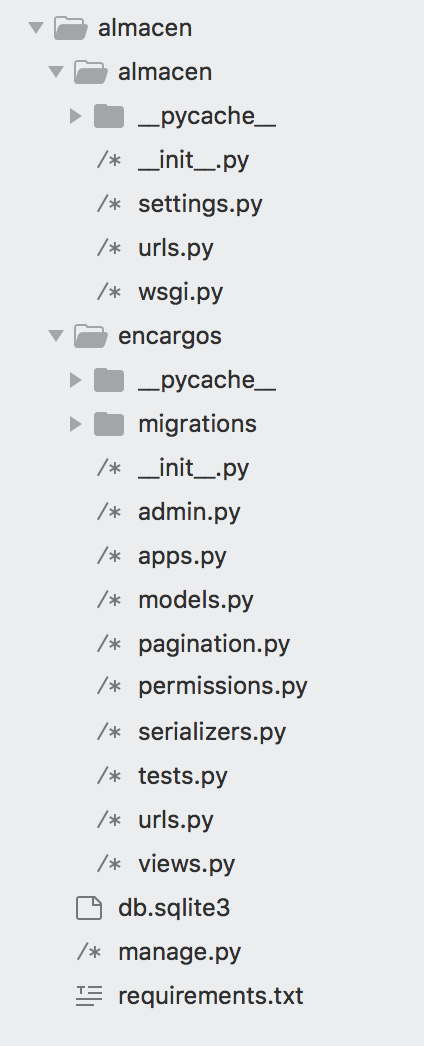
\includegraphics[width=4cm]{images/estructura_djangoREST.png}
	\end{center}
	\caption{Estructura Django API RESTful}
	\label{fig:EstructuraDjangoAPI}
\end{figure}


\chapter{Compoñentes Hardware}
\section{Arduino Mega 2560}

Arduino Mega 2560 está baseado no microcontralador ATmega2560. Ten 54 pines de entrada/saída dixitais (dos cales 15 pódense empregar como saídas PWM), 16 entradas analóxicas, 4 UART (portas de serie de hardware), un oscilador de cristal de 16 MHz, unha conexión USB, unha toma de enerxía, un encabezado ICSP, e un botón de reset. Contén todo o necesario para soportar o desenvolvimento de aplicacións para este microcontrolador; simplemente conéctase a unha computadora con un cable USB ou aliméntase cun adaptador AC-to-DC ou batería para comezar. 

\begin{figure}[H]
	\begin{center}
		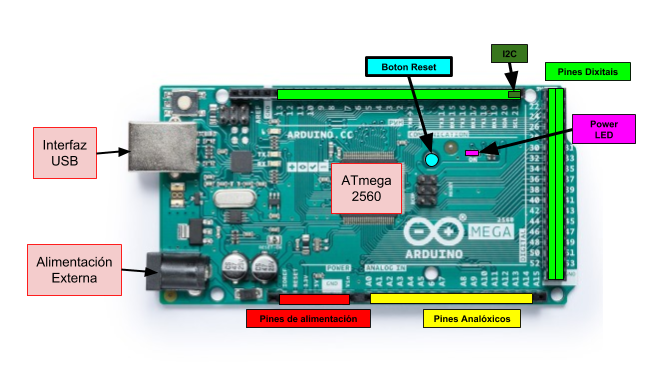
\includegraphics[width=12cm]{images/pinoutMega2560.png}
	\end{center}
	\caption{Arduino Mega 2560 \cite{wArduino}}
	\label{fig:ArduinoMega}
\end{figure}

\subsection{Alimentación eléctrica}

Pode ser alimentado a través da conexión USB ou cunha fonte de alimentación externa. A fonte de enerxía selecciónase automaticamente. 

A placa pode funcionar nunha fonte externa de 6 a 20 voltios. Se se alimenta con menos de 7V, pode volverse inestable, mentres que se se usa máis de 12V, pode sobrequentarse e dañarse. O rango recomendado é de 7 a 12V.

Os pines de alimentación son os seguintes:

\begin{itemize}
\item \textbf{Vin}: A tensión de entrada á placa cando está a usar unha fonte de enerxía externa. Pódese alimentar a través do porto USB ou a través deste pin.
\item \textbf{5V}: Proporciona 5V desde o regulador da placa.
\item \textbf{3V3}: Unha fonte de 3,3V xerada polo regulador da placa. O amperaxe máximo actual é de 50 mA.
\item \textbf{GND}: Pines de terra.
\item \textbf{IOREF}: Proporciona VREF coa que funciona o microcontrolador. Ten configurada unha protección que le esa tensión e selecciona traballar con 3,3V ou con 5V.
\end{itemize}

\section{Módulos ou periféricos}

\subsection{Pantalla LCD}

Para visualizar os pedidos dos operarios e xestionalos, empregarase unha pantalla LCD alfanumérica de 4 filas e 40 columnas modelo Midas MC44005A6W-FPTLW. \cite{pantalla} 

\begin{figure}[H]
	\begin{center}
		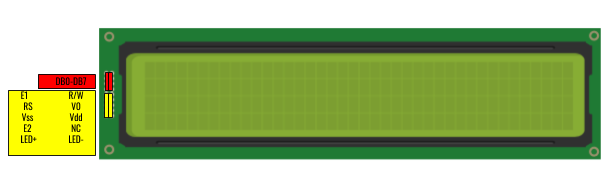
\includegraphics[width=16cm]{images/pinoutPantalla.png}
	\end{center}
	\caption{Pin out pantalla LCD}
	\label{fig:PantallaLCD}
\end{figure}

\begin{table}[H]
\centering
\begin{tabular}{@{}cc@{}}
\textbf{SÍMBOLO} & \textbf{FUNCIÓN}             \\ \midrule
DB7-DB0          & Bus Data Line                \\
E1               & Enable Signal                \\
R/W              & Data Read / Write            \\
RS               & Register Select Signal       \\
V0               & Contrast Adjust              \\
Vss              & GND                          \\
Vdd              & Power supply for LCM (+5.0V) \\
E2               & Enable Signal                \\
NC               & No connection                \\
LED+             & Power supply for BKL (+5.0V) \\
LED-             & Power supply for BKL (0V)    \\ \bottomrule
\end{tabular}
\caption{Pines pantalla LCD}
\label{my-label}
\end{table}

A conexión da pantalla coa placa Arduino Mega vai ser da seguinte maneira:

\begin{figure}[H]
	\begin{center}
		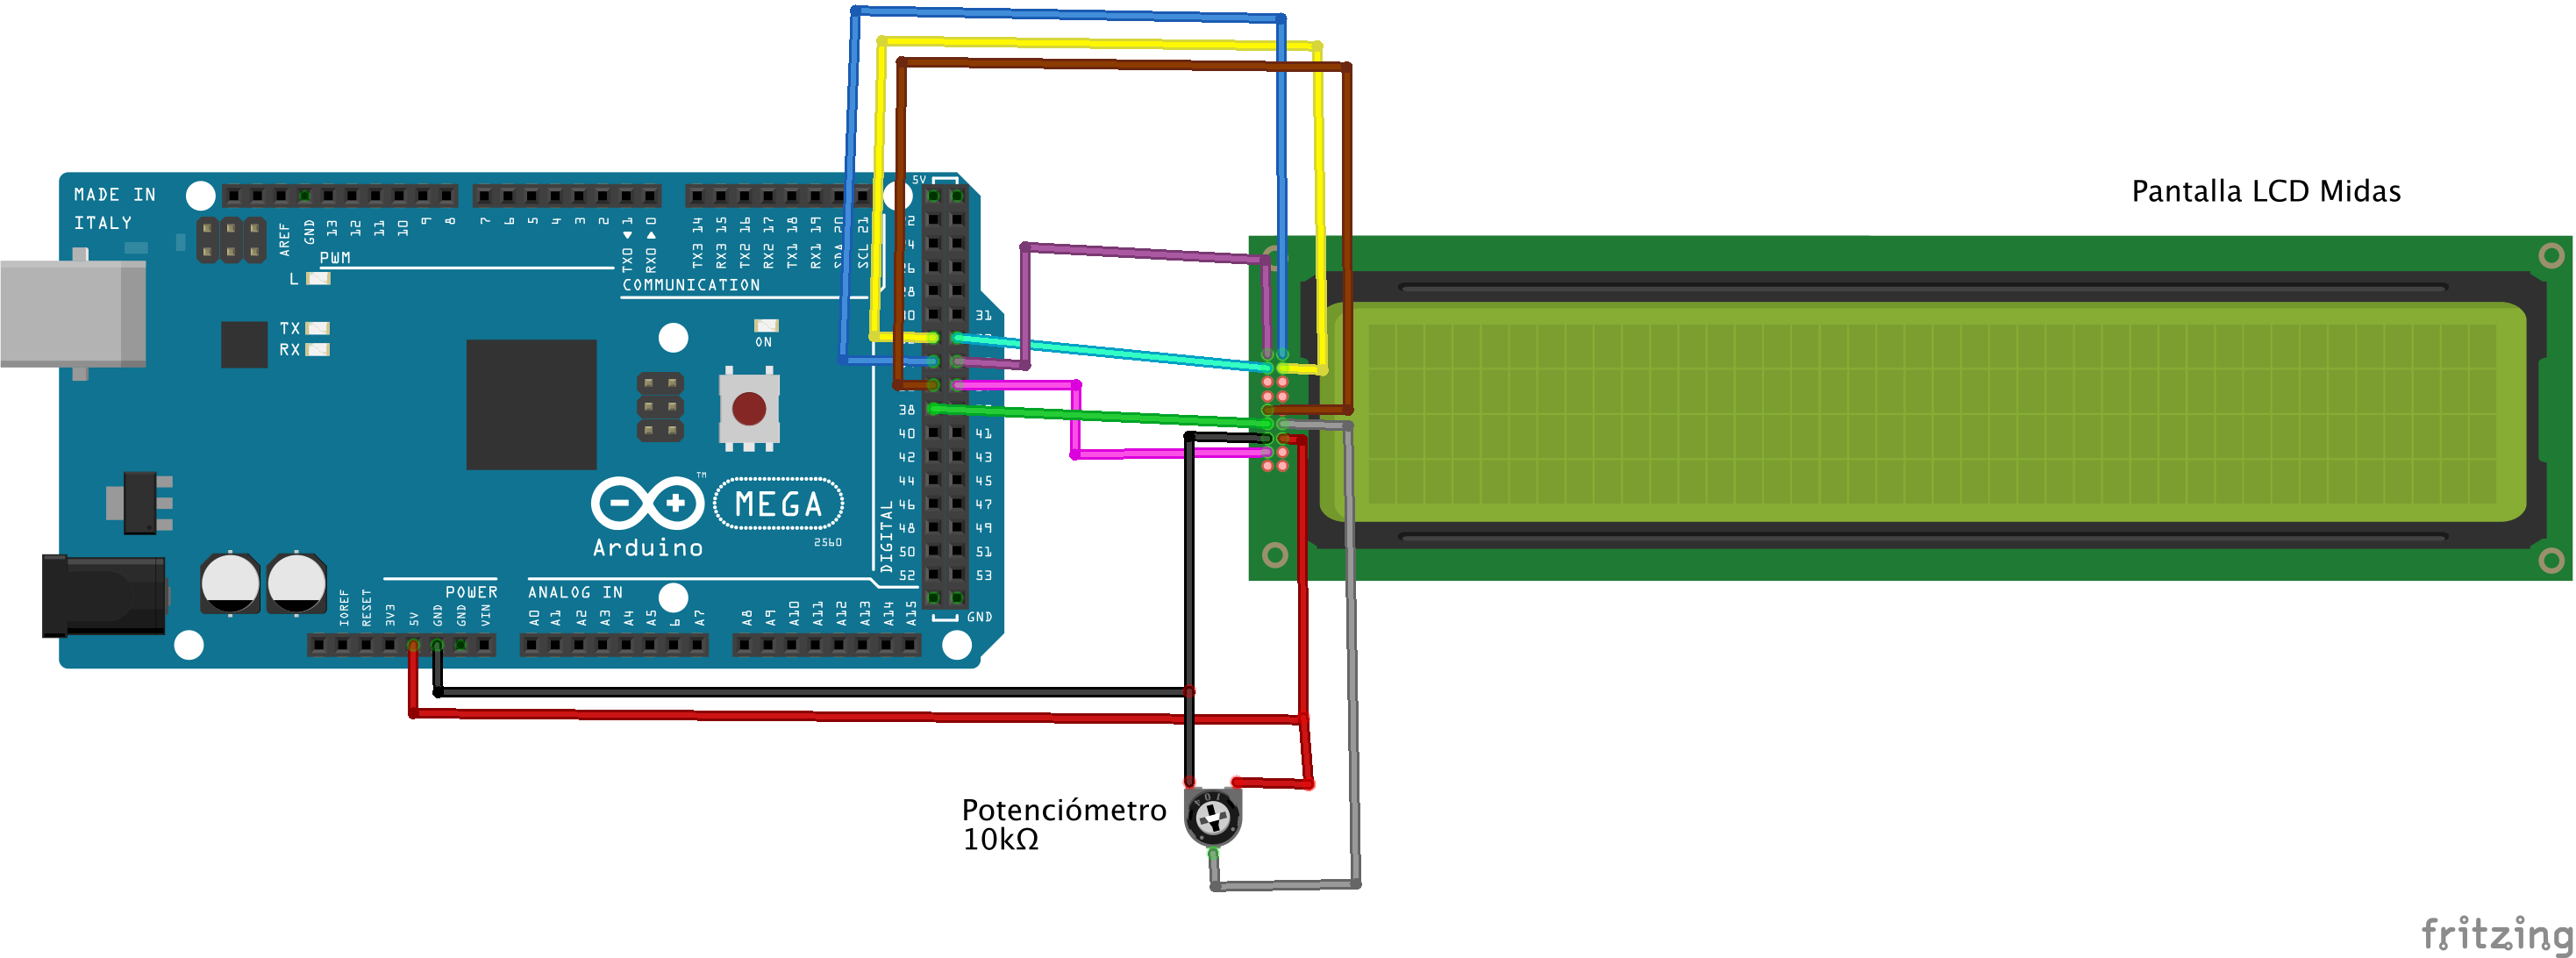
\includegraphics[width=15cm]{images/conexionArduinoLCD.png}
	\end{center}
	\caption{Conexión placa Arduino Mega con pantalla LCD Midas}
	\label{fig:ConexionPantalla}
\end{figure}

\begin{table}[h]
\begin{center}
\begin{tabular}{|c|c|c|}
\hline
Arduino & Pantalla Midas & Color \\
\hline
32 & DB4 & Amarelo \\
\hline
33 & DB5 & Cian\\
\hline
34 & DB6 & Azul \\
\hline
35 & DB7 & Morado \\
\hline
36 & E1 & Marrón \\
\hline
37 & E2 & Rosa \\
\hline
38 & RS & Verde \\
\hline
5V & Vdd & Vermello \\
\hline
GND & Vss & Negro \\
\hline
\end{tabular}
\caption{Conexión pines entre Arduino e Pantalla LCD Midas}
\label{TablaArduinoPantalla}
\end{center}
\end{table}

Para o control de alimentación, e, polo tanto, para o control de brillo da pantalla, vaise añadir un potenciómetro de 10k que ten o esquema reflexado na figura \ref{fig:ConexionPantalla} e os seguintes pines:

\begin{table}[htbt]
\begin{center}
\begin{tabular}{|c|c|c|}
\hline
Potenciómetro & Pantalla Midas & Arduino\\
\hline
IN & Vdd & 5V \\
\hline
OUT & V0 & -\\
\hline
\end{tabular}
\caption{Conexión do potenciómetro}
\label{TablaPotenciometro}
\end{center}
\end{table}

\subsection{Teclado Matricial}

Para poder indicarlle ó terminal que se completou unha caixa, vaise usar un teclado matricial 4x4 modelo Storm 720TFX Series. \cite{teclado}

\begin{figure}[H]
	\begin{center}
		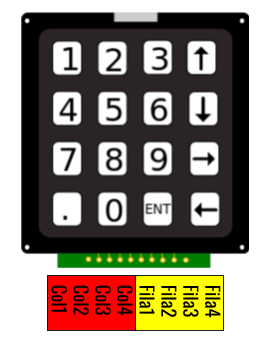
\includegraphics[scale=0.6]{images/pinoutTeclado.png}
	\end{center}
	\caption{Pinout Teclado 4x4}
	\label{fig:TecladoStorm}
\end{figure}

A conexión con Arduino vai ser da seguinte maneira:

\begin{figure}[H]
	\begin{center}
		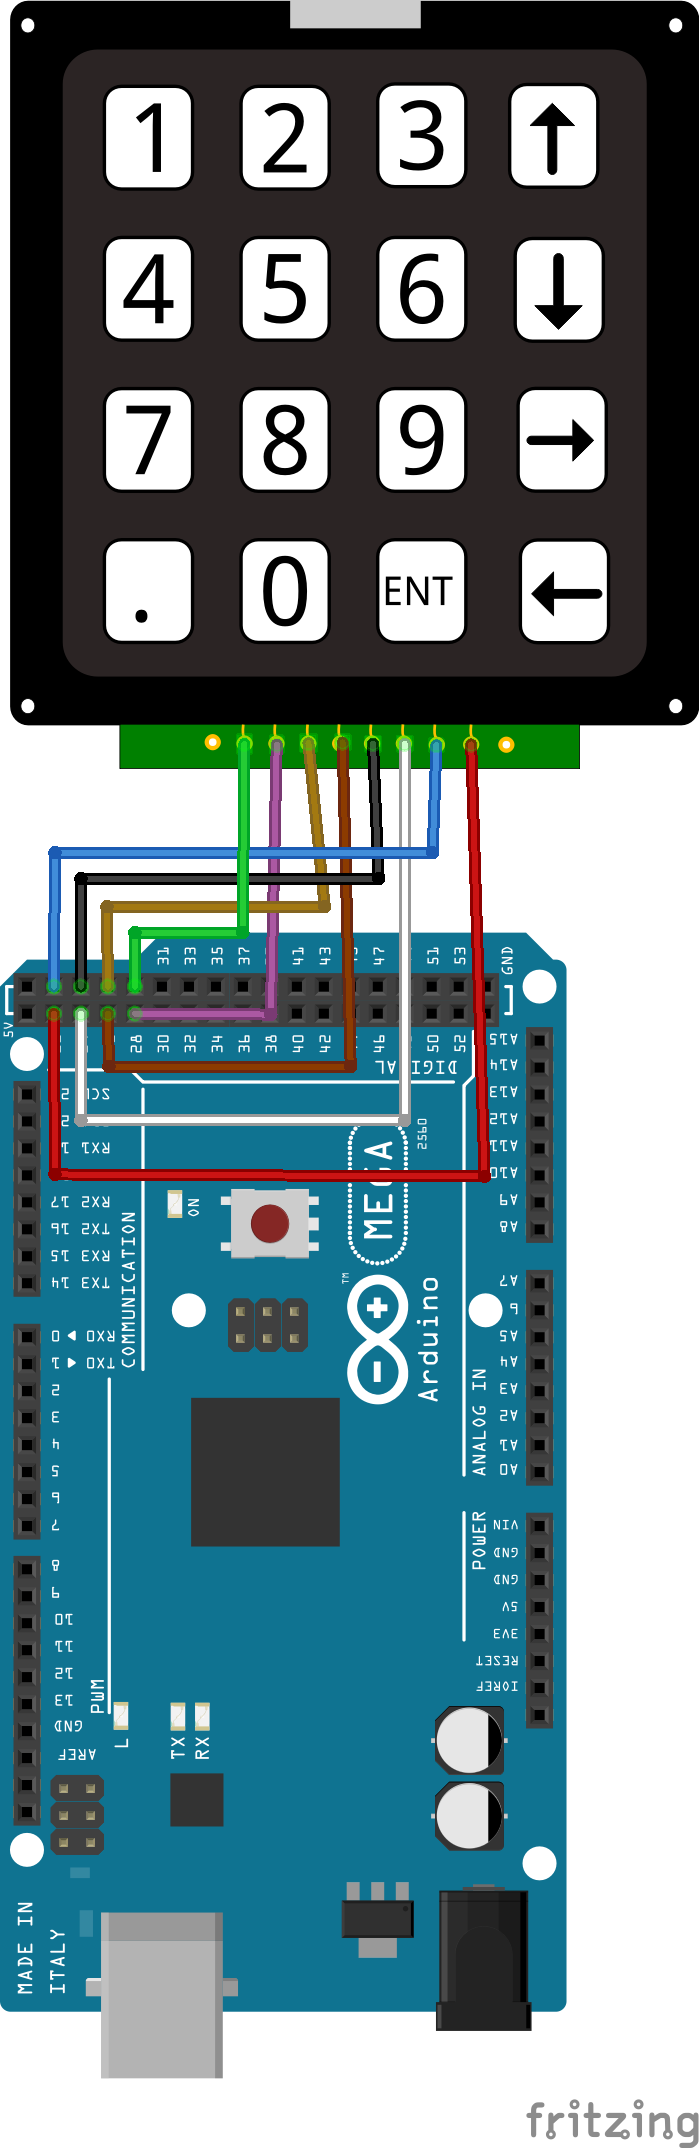
\includegraphics[scale=0.75]{images/conexionArduinoKeypad.png}
	\end{center}
	\caption{Conexión placa Arduino Mega con teclado 4x4 Matrix}
	\label{fig:ConexionESP8266}
\end{figure}

\begin{table}[H]
\begin{center}
\begin{tabular}{|c|c|c|}
\hline
Arduino & Keypad Storm & Color \\
\hline
22 & Col1 & Vermello \\
\hline
23 & Col2 & Azul\\
\hline
24 & Col3 & Blanco \\
\hline
25 & Col4 & Negro \\
\hline
26 & Fila1 & Marrón \\
\hline
27 & Fila2 & Ocre\\
\hline
28 & Fila3 & Verde \\
\hline
29 & Fila4 & Morado \\
\hline
\end{tabular}
\caption{Conexión pines entre Arduino e Teclado 4x4}
\label{TablaArduinoKeypad}
\end{center}
\end{table}

\subsection{ESP8266}

É un microprocesador de baixo custo con WiFi integrado fabricado por Espressif. Supuxo unha revolución á hora de conectar o Arduino a WiFi, xa que as placas existentes eran demasiado caras, como por exemplo WiFi Shield (arredor duns 90€).

Ademáis, pode comportarse como un procesador completo, con moita máis potencia que a maioría das placas Arduino.

Existen moitos modelos de placas que integran ESP8266; o módulo ESP01 é un dos primeiros en aparecer co chip ESP8266 é un dos módulos máis sinxelos e baratos. \cite{ESP2}

\begin{figure}[H]
	\begin{center}
		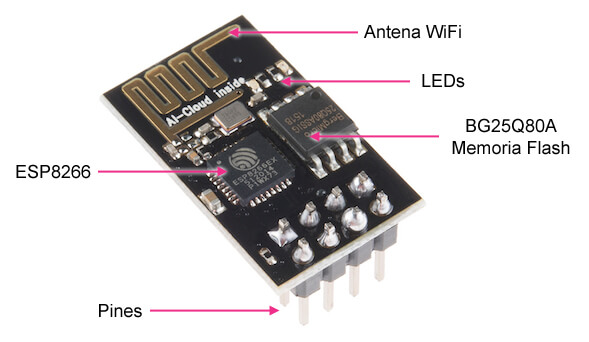
\includegraphics[width=10cm]{images/esp8266_conexion.jpg}
	\end{center}
	\caption{Esquema módulo ESP8266}
	\label{fig:EsquemaESP8266}
\end{figure}

En canto a comunicación WiFi, o ESP01 ten comunicación integrada 802.11  b/g/n, incluidos modos  Wi-Fi  Direct (P2P) e  soft-Ap. Inclúe unha pila de  TCP/IP completa, o que libera da maior parte do traballo de comunicación ó procesador.

\subsubsection{Esquema Eléctrico}

A conexión co módulo ESP8266 é bastante sinxela en comparación cos demáis compoñentes íntegros no proxecto. Ten os seguintes pines:

\begin{figure}[H]
	\begin{center}
		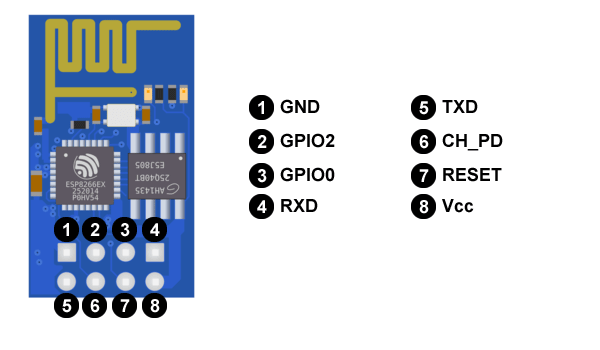
\includegraphics[width=10cm]{images/pines-esp01.png}
	\end{center}
	\caption{Pines módulo ESP8266}
	\label{fig:PinesESP8266}
\end{figure}

\begin{enumerate}
\item GND é a toma de terra.
\item GPIO2 é unha entrada/saida de propósito xeral. É o pin dixital número 2.
\item GPIO0 é unha entrada/saida de propósito xeral. É o pin dixital número 0.
\item RxD é o pin por onde se reciben os datos no porto serie. Pódese usar como pin dixital GPIO: sería o número 3.
\item TxD é o pin por onde se transmiten os datos no porto serie. Pódese usar como pin dixital GPIO: sería o número 1.
\item CH\_PD é o pin que o apaga ou encende: se está a 0V (LOW) apágase a 3,3V (HIGH), encéndese.
\item RESET é o pin que o resetea: se está a 0V (LOW) resetéase.
\item Vcc é por onde se alimenta. Funciona a 3,3 V.
\end{enumerate}

A única dificultade que imos ter vai ser á hora de alimentalo, xa que ten unha tensión de alimentación de 3,3V. En ningún caso pode alimentarse cunha tensión superior a 3,6 V, ou dañaríamolo.

A conexión coa placa vai ser a seguinte:

\begin{figure}[H]
	\begin{center}
		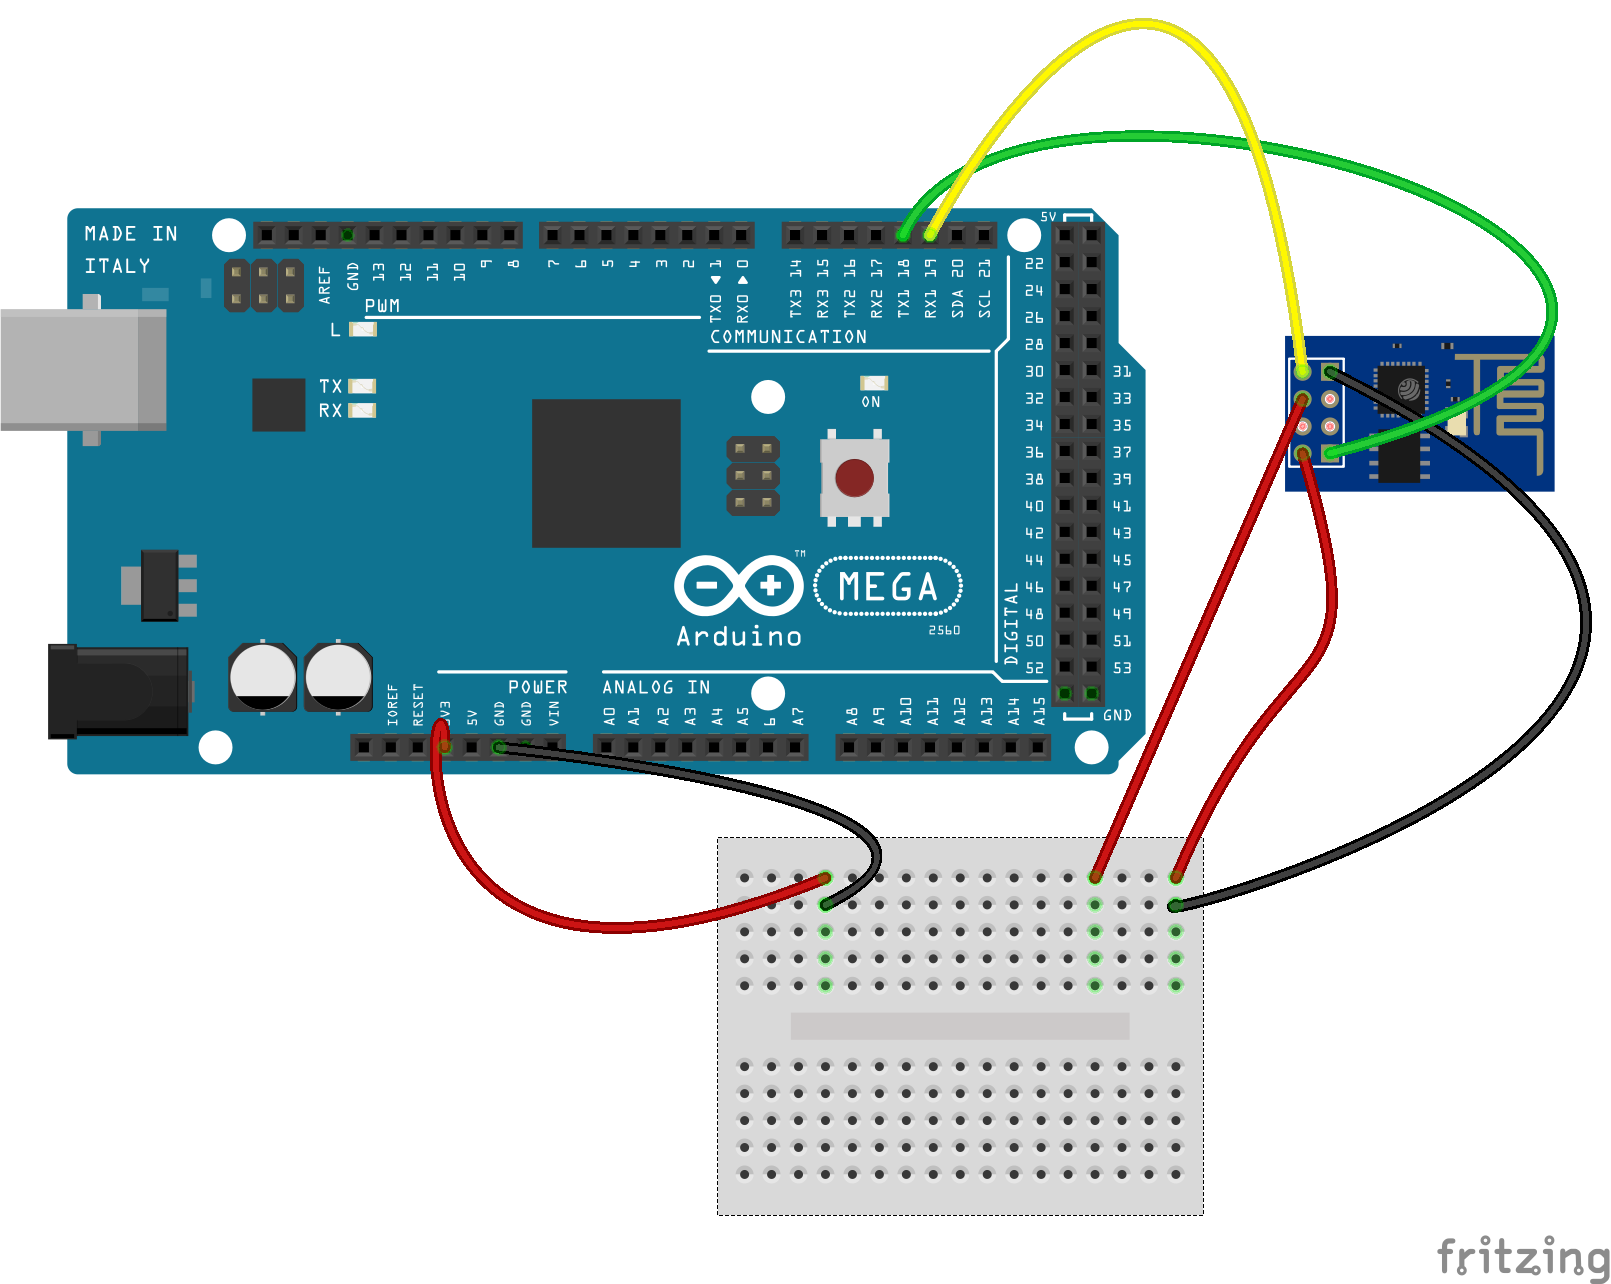
\includegraphics[width=10cm]{images/conexionArduinoESP8266_WiFiEsp.png}
	\end{center}
	\caption{Conexión placa Arduino Mega con módulo ESP8266}
	\label{fig:ConexionESP8266}
\end{figure}

\begin{table}[htbt]
\begin{center}
\begin{tabular}{|c|c|}
\hline
Arduino & ESP8266 \\
\hline
3,3V & Vcc \\
\hline
GND & GND \\
\hline
TX1(18) & RxD \\
\hline
Rx1(19) & TxD \\
\hline
3,3V & CH\_PD \\
\hline
\end{tabular}
\caption{Conexión pines entre Arduino e ESP8266}
\label{TablaArduinoESP8266_WiFiEsp}
\end{center}
\end{table}

\chapter{Compoñentes software}

Neste capítulo vaise dividir en dúas partes: a parte de programación do Arduino Mega 2560 e a parte da creación de servicios REST.

\section{Programa Arduino}

\subsection{Diagrama de fluxo}

Como se pode ver na seguinte figura \ref{fig:FluxoPrincipal} o código está dividido en \textit{setup}, que é a inicialización da placa Arduino e se vai executar so unha vez, e \textit{loop}, que é un bucle que se vai executar continuamente.

\begin{figure}[H]
	\begin{center}
		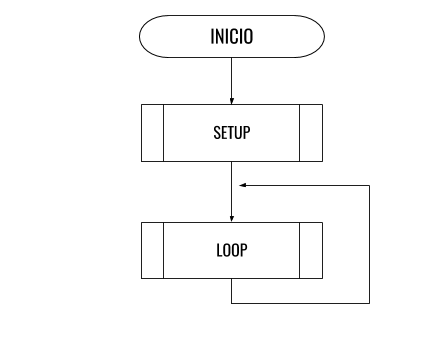
\includegraphics[width=5cm]{images/diagrama_flujo_inicio.png}
	\end{center}
	\caption{Diagrama de fluxo do programa principal Arduino}
	\label{fig:FluxoPrincipal}
\end{figure}

\begin{figure}[H]
	\begin{center}
		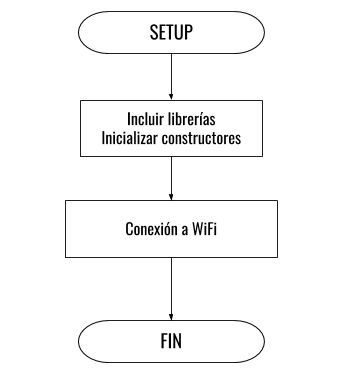
\includegraphics[width=6cm]{images/diagrama_flujo_setup.png}
	\end{center}
	\caption{Diagrama de fluxo de SETUP Arduino}
	\label{fig:FluxoSETUP}
\end{figure}

\begin{figure}[H]
	\begin{center}
		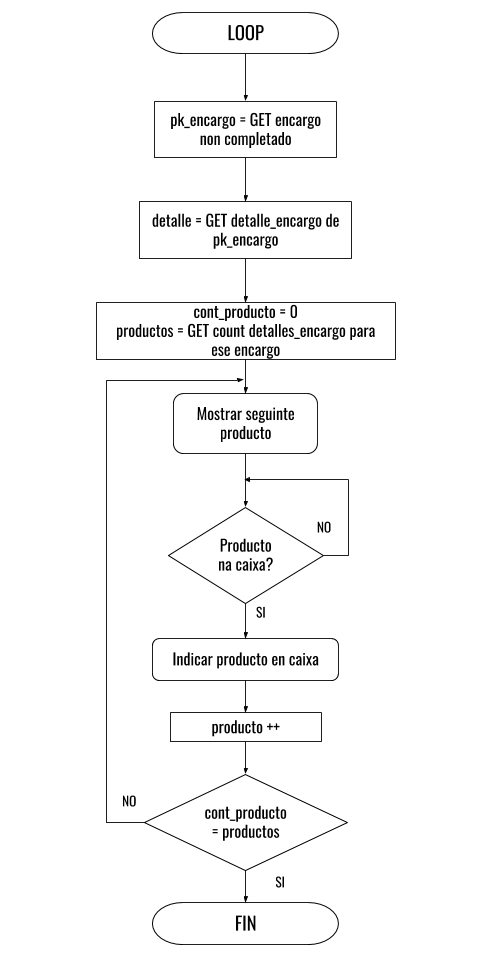
\includegraphics[width=8cm]{images/diagrama_flujo_loop.png}
	\end{center}
	\caption{Diagrama de fluxo de LOOP Arduino}
	\label{fig:FluxoLOOP}
\end{figure}
 
\subsection{Pantalla LCD}

Vaise usar a clase \textit{PantallaMidas} para manexar a pantalla LCD, reflexada no documento ANEXO. 

Ten os seguintes métodos:

\begin{itemize}
    \item \textit{PantallaMidas(int DB4, int DB5, int DB6, int DB7, int E1, int E2, int RS)}: Constructor da clase que se lle pasa por parámetros que señais Arduino están conectadas ás señais da pantalla. Inicialízase en \textit{setup()}.
    \item \textit{void configura()}: Método que configura a pantalla. Vai ter unha configuración de bus de 4bits. Ten o seguinte diagrama de fluxo:
    \begin{figure}[H]
    	\begin{center}
    		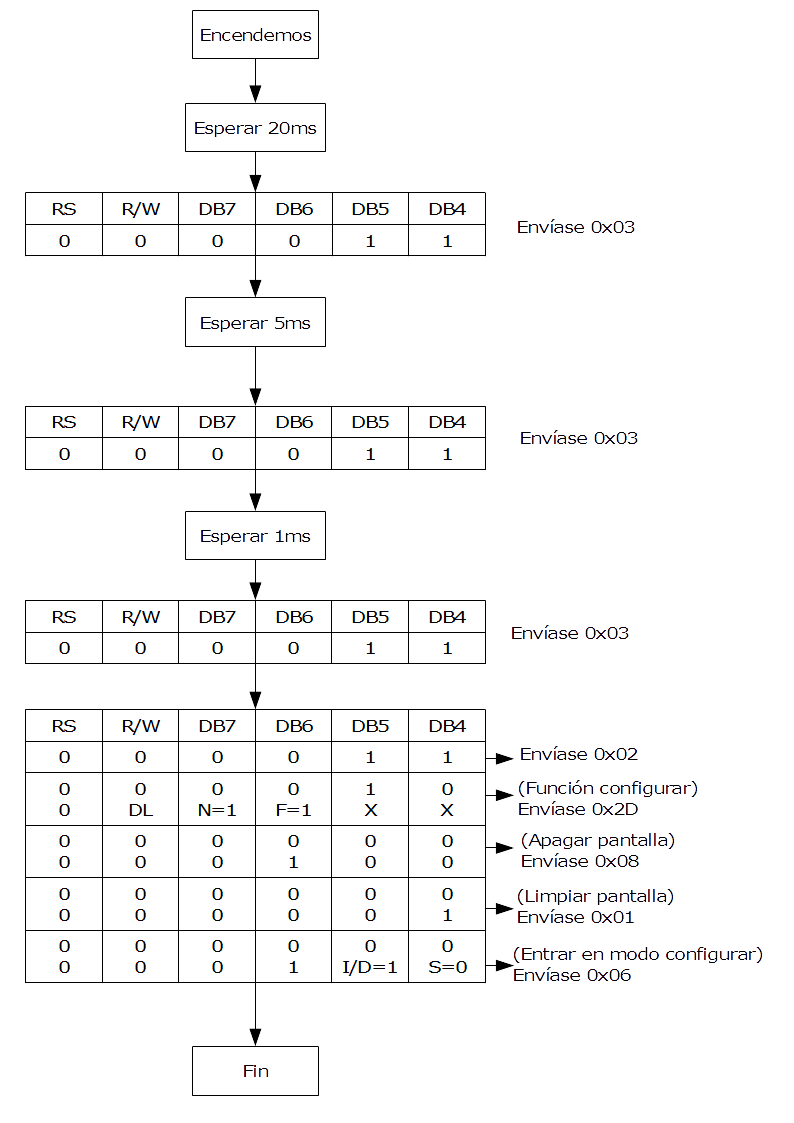
\includegraphics[scale=0.6]{images/inicializar_lcd.png}
    	\end{center}
    	\caption{Diagrama de Fluxo inicilización pantalla}
    	\label{fig:DiagramaFlujoPantalla}
    \end{figure}
    \item \textit{void borra()}: Método que fai un ``clean'' da pantalla.
    \item \textit{void posiciona(int fila, int columna)}: Método que posiciona o cursor na pantalla na localización indicada polos parámetros fila e columna.
    \item \textit{ void escribeCadea(const char * cadea)}: Método que escribe o que lle pasas por parámetro na posición na que esté o cursor.
    \item \textit{void mostraCursor(int muestrao)}: Método que mostra ou non o cursor según o que lle pases por parámetro.
\end{itemize}

\subsection{Teclado Matricial}

Para usar este compoñente, elaborouse unha clase en C++ chamada \textit{Teclado4x4} que esta reflexada no documento ANEXO.

Contén as seguintes funcións:

\begin{itemize}
    \item \textit{Teclado4x4(int F1, int F2, int F3, int F4, int C1, int C2, int C3, int C4, char *caracteres)}: Constructor da clase que se lle pasa por parámetros os pines e os caracteres asociados. Inicialízase en \textit{setup()} dentro do programa principal.
    \item \textit{void configura()}: Método que configura o teclado para o seu uso.
    \item \textit{int comproba()}: Método que comproba se se pulsou unha determinada tecla. Devolve o caracter pulsado.
\end{itemize}

Para manexar as clases \textit{Teclado4x4} e \textit{PantallaMidas}, elaborouse unha clase chamada \textit{Consola}. Está reflexada no documento ANEXOS.

\subsection{ESP6288 ESP-01}

Este módulo WiFi comunícase coa placa Arduino mediante comandos AT por serie. Para manexalos, vaise usar unha librería Open Source \textit{WiFiEsp}\cite{esp}.

A continuación mostraranse os comandos usados no proxecto ligado á función da librería mencionada antes:

\begin{table}[h!]
\centering
\resizebox*{16cm}{!}{
\begin{tabular}{@{}lllllc@{}}
\toprule
\multicolumn{1}{c}{Comando} & \multicolumn{1}{c}{Descripción} & \multicolumn{1}{c}{Resposta} & \multicolumn{1}{c}{Configuración} & \multicolumn{1}{c}{Parámetros} & \multicolumn{1}{l}{Función WiFiEsp} \\ \midrule
AT+CWMODE & \begin{tabular}[c]{@{}l@{}}Configura o \\ módulo WiFi\end{tabular} & Mode set & AT+CWMODE=\textless{}Modo\textgreater{} & \begin{tabular}[c]{@{}l@{}}Modo 1 = Sta\\           2 = AP\\           3 = both\end{tabular} & init() \\
AT+CWJAP & \begin{tabular}[c]{@{}l@{}}Conéctase ó \\ Punto de Acceso\end{tabular} & OK & AT+CWJAP=\textless{}ssid\textgreater{},\textless{}pwd\textgreater{} & \begin{tabular}[c]{@{}l@{}}ssid = Nome de rede\\ pwd = Contrasinal\end{tabular} & begin(ssid, pwd) \\
AT+CIPSTATUS & \begin{tabular}[c]{@{}l@{}}Estado da conexión\\ TCP/IP\end{tabular} & STATUS=\textless{}sta\textgreater{} & \multicolumn{1}{c}{CIPSTATUS} &  & status() \\
AT+CIPSTART & \begin{tabular}[c]{@{}l@{}}Configura a \\ conexión como \\ TCP ou UDP\end{tabular} & OK & \multicolumn{1}{c}{\begin{tabular}[c]{@{}c@{}}AT+CIPSTART=\textless{}type\textgreater{},\\ \textless{}addr\textgreater{},\textless{}port\textgreater{}\end{tabular}} & \begin{tabular}[c]{@{}l@{}}type=``TCP'' ou ``UDP''\\ addr=IP do servidor\\ port=Porto do servidor\end{tabular} & connect(addr,port) \\
AT+CIPSEND & Envía data & "\textgreater{}" para enviar datos & AT+CIPSEND=\textless{}lenght\textgreater{} & \begin{tabular}[c]{@{}l@{}}lenght=tamaño do dato\\ a enviar\end{tabular} & write(lenght) \\
+IPD & Recibe data & + IPD \textless{}lenght\textgreater{} & +IPD &  & read() \\
AT+CIPCLOSE & \begin{tabular}[c]{@{}l@{}}Para a conexión\\ TCP ou UDP\end{tabular} &  & AT+CIPCLOSE &  & stop() \\ \bottomrule
\end{tabular}}
\caption{Comandos AT básicos}
\label{TablaComandosAT}
\end{table}

Para realizar conexión a un punto de acceso (AP) como para facer consultas a base de datos creada por Django API REST, implementouse a clase \textit{ConnectEsp}, que ten os seguintes métodos:

\begin{itemize}
    \item \textit{connectAP()}: realiza a conexión a un punto de acceso.
    \item \textit{httpRequest(char message[])}: realiza a consulta GET contra a base de datos, pasándolle como parámetro o método HTTP.
    \item \textit{bool get\_Encargo\_completado\_django()}: le do servidor se un encargo está completado e devolve unha variable tipo bool se é afirmativo.
    \item \textit{int get\_producto\_Encargo\_django()}: le do servidor cantos productos hai para o encargo non completado, devolvento unha variable tipo int con ese numero.
    \item \textit{get\_Localizacion\_django(int num\_producto)}: le os campos da tabla producto, pasandolle por parametro o numero do producto.
    \item \textit{post\_encargo\_completado()}: modifica o campo ``completado'' a true da tabla Encargos.
\end{itemize}

Para manexar os datos recibidos das consultas, vaise usar outra librería Open Source chamada \textit{ArduinoJSON}, que vai permitir tanto xerar como dividir datos tipo JSON \cite{Json}. Úsase da seguinte maneira:

\begin{minted}{cpp}
  const char* json = "{\"sensor\":\"gps\",\"time\":1351824120}";
  //créase unha variable tipo array de char que contén
  //os datos JSON que queremos dividir
  
  StaticJsonBuffer<100> jsonBuffer;
  //declárase o uso de memoria estática de tamaño 100
  
  JsonObject& root = jsonBuffer.parseObject(json);
  //divídese o código json creado e métese na variable root
  
  char* sensor = root["sensor"]; 
  //métese nun array de char o campo sensor
  int time = root["time"]        
  //métese nun int o campo time
\end{minted}

\section{Django RESTful Web Framework}

É unha librería que vai permitir construir un API REST sobre Django. Ofrece unha diversidade de métodos e funcións para a xestión dos recursos.

Esta librería é totalmente portable; podese usar tanto con Windows, Linux ou Mac OSX. Neste proxecto vaise usar o sistema operativo MacOs Hight Sierra.

A continuación móstrase como creala:

\subsection{Crear directorio base}

Vaise crear un directorio onde vai estar contido o código. Ábrese unha ventana de terminal:

\begin{minted}{bash}
  $ mkdir tfg_django  #creamos unha carpeta para 
                      #o proxecto chamado tfg_django
  $ cd tfg_django     #accedemos a esa carpeta
\end{minted}

\subsection{Configurar entorno virtual}

Esto vai permitir aislar as dependencias do proxecto, eliminando os conflictos de librerías locais do sistema.
\begin{minted}{bash}
  $ virtualenv tfg_django
  $ source env/bin/activate #esto activará o noso entorno virtual.
\end{minted}

A continuación, instalaranse os paquetes necesarios.

\begin{minted}{bash}
  $ pip install django #instalar o paquete de django
  $ pip install djangorestframework #instalar o paquete de 
                                    #Django Rest Framework
\end{minted}

\subsection{Crear proxecto e configuración inicial}

Vaise crear o proxecto dentro do directorio base e inicializar a configuración. A API vaise chamar \textit{almacen} e vaise crear unha aplicación que se chamará \textit{encargos}.

\begin{minted}{bash}
  $ django-admin.py startproject almacen
  $ cd encargos
  $ django-admin.py startapp encargos
\end{minted}

Vaise modificar o arquivo \textit{almacen/settings.py} para añadir a aplicación creada mais a librería.

\begin{minted}{python}
INSTALLED_APPS = (
    ...
    'rest_framework',
    'encargos',
)
\end{minted}

\subsection{Crear Models}

Vaise modificar o arquivo \textit{encargos/models.py} para crear os modelos.

\begin{minted}{python}
from django.db import models

class Encargo(models.Model):                          
#creamos tabla Encargo                     

    operario = models.ForeignKey(                      
        'auth.User',
        related_name='encargo',
        on_delete=models.CASCADE)
    #campo operario
    completado = models.BooleanField(default=False)  
    #campo completado tipo bool

    class Meta:                                      
        ordering = ('pk',)
        #ordena esta tabla polo id


class Producto(models.Model):
    AREA1 = '1'
    AREA2 = '2'
    AREAS = (
        (AREA1, 'Area 1'),
        (AREA2, 'Area 2'),
    )
    name = models.CharField(max_length=50)
    localizacion = models.CharField(
        max_length=2,
        choices=AREAS,
        default=AREA1, 
    )

    class Meta: 
        ordering = ('name',)

    def __str__(self):
        return self.name                      
    #getter que devolve o nome do producto


class Detalle_Encargo(models.Model):
    producto = models.ForeignKey(
        Producto, 
        related_name='producto', 
        on_delete=models.CASCADE)
    encargo = models.ForeignKey(
        Encargo, 
        on_delete=models.CASCADE)
    cantidade = models.IntegerField()
)
\end{minted}

Para xerar os cambios realizados nos modelos hai que facer migracións. Para iso, usaranse os comandos:

\begin{minted}{bash}
  $ python manage.py makemigrations 
  $ python manage.py migrate
\end{minted}

\subsection{Crear ModelSerializers}

Créase un serializer en \textit{encargos/serializers.py}. 

\begin{minted}{python}
from rest_framework import serializers
from encargos.models import Encargo
from encargos.models import Producto
from encargos.models import Detalle_Encargo
from django.contrib.auth.models import User


class UserEncargoSerializer(serializers.HyperlinkedModelSerializer):
    class Meta:
        model = Encargo          
        fields = (                    #campos que vai ter
            'url',
            'name')


class UserSerializer(serializers.HyperlinkedModelSerializer):
    encargos = UserEncargoSerializer(many=True, read_only=True)

    class Meta:
        model = User
        fields = (
            'url', 
            'pk',
            'username',
            'encargos',
            'password'
        )

class EncargoSerializer(serializers.HyperlinkedModelSerializer):

    class Meta:
        model = Encargo
        fields = (
            'url',
            'pk',
            'created',
            'completado'
    )


class ProductoSerializer(serializers.HyperlinkedModelSerializer):
    localizacion = serializers.ChoiceField(choices=Producto.AREAS)
    area_description = serializers.CharField(
        source='get_area_display', 
        read_only=True
    )
    class Meta:
        model = Producto
        fields = (
            'url',
            'pk',
            'name',
            'localizacion',
            'area_description',
        )

class Detalle_EncargoSerializer(serializers.ModelSerializer):
    localizacion_producto = ProductoSerializer(many=True, read_only=True)
    encargo_completado = EncargoSerializer(many=True, read_only=True)
    class Meta:
        model = Detalle_Encargo
        fields = (
            'url',
            'pk',
            'encargo',
            'producto',
            'cantidade',
            'localizacion_producto',
            'encargo_completado'
        )
\end{minted}

\subsection{Vistas normales en Django}

Unha vez creado o serializador, vaise crear a API usando vistas funcionais ou vistas simples en Django. Para eso, vaise modificar o arquivo \textit{encargos/views.py}.

\begin{minted}{python}
from encargos.models import Encargo
from encargos.models import Producto
from encargos.models import Detalle_Encargo
from encargos.serializers import EncargoSerializer
from encargos.serializers import ProductoSerializer
from encargos.serializers import Detalle_EncargoSerializer
from rest_framework import generics
from rest_framework.response import Response
from rest_framework.reverse import reverse
from django.contrib.auth.models import User
from encargos.serializers import UserSerializer
from rest_framework import permissions
from encargos.permissions import IsOperarioOrReadOnly


class UserList(generics.ListAPIView):
    queryset = User.objects.all()
    serializer_class = UserSerializer
    name = 'user-list'


class UserDetail(generics.RetrieveAPIView):
    queryset = User.objects.all()
    serializer_class = UserSerializer
    name = 'user-detail'

class EncargoList(generics.ListCreateAPIView):
    queryset = Encargo.objects.all()
    serializer_class = EncargoSerializer
    name = 'encargo-list'


class EncargoDetail(generics.RetrieveUpdateDestroyAPIView):
    queryset = Encargo.objects.all()
    serializer_class = EncargoSerializer
    name = 'encargo-detail'


class ProductoList(generics.ListCreateAPIView):
    queryset = Producto.objects.all()
    serializer_class = ProductoSerializer
    name = 'producto-list'


class ProductoDetail(generics.RetrieveUpdateDestroyAPIView):
    queryset = Producto.objects.all()
    serializer_class = ProductoSerializer
    name = 'producto-detail'
    

class Detalle_EncargoList(generics.ListCreateAPIView):
    queryset = Detalle_Encargo.objects.all()
    serializer_class = Detalle_EncargoSerializer
    name = 'detalle_encargo-list'


class Detalle_EncargoDetail(generics.RetrieveUpdateDestroyAPIView):
    queryset = Detalle_Encargo.objects.all()
    serializer_class = Detalle_EncargoSerializer
    name = 'detalle_encargo-detail'
    

class ApiRoot(generics.GenericAPIView):
    name = 'api-root'
    def get(self, request, *args, **kwargs):
        return Response({
            'productos': reverse(ProductoList.name, request=request),
            'detalle_encargo': reverse(
                    Detalle_EncargoList.name, 
                    request=request
            ),
            'encargos': reverse(EncargoList.name, request=request),
            'users': reverse(UserList.name, request=request),
            })
\end{minted}

Finalmente, agrégase as url para poder mostrar os servicios. Modificase o arquivo \textit{encargos/urls.py}.
\begin{minted}{python}
from django.conf.urls import url
from encargos import views


urlpatterns = [
    url(r'^encargos/$', 
        views.EncargoList.as_view(),
        name=views.EncargoList.name),
    url(r'^encargos/(?P<pk>[0-9]+)/$', 
        views.EncargoDetail.as_view(),
        name=views.EncargoDetail.name),
    url(r'^productos/$', 
        views.ProductoList.as_view(),
        name=views.ProductoList.name),
    url(r'^productos/(?P<pk>[0-9]+)/$', 
        views.ProductoDetail.as_view(),
        name=views.ProductoDetail.name),
    url(r'^detalle_encargo/$', 
        views.Detalle_EncargoList.as_view(),
        name=views.Detalle_EncargoList.name),
    url(r'^detalle_encargo/(?P<pk>[0-9]+)/$', 
        views.Detalle_EncargoDetail.as_view(),
        name=views.Detalle_EncargoDetail.name),
    url(r'^users/$',
        views.UserList.as_view(),
        name=views.UserList.name),
    url(r'^users/(?P<pk>[0-9]+)/$',
        views.UserDetail.as_view(),
        name=views.UserDetail.name),
    url(r'^$',
        views.ApiRoot.as_view(),
        name=views.ApiRoot.name),
]
\end{minted}

\subsection{Visualización API}

Para mostrar a API, levantarase o servidor con:

\begin{minted}{bash}
  $ python manage.py runserver 
\end{minted}

Por defecto, o servidor lanzarase en \textit{http://127.0.0.0.1:8000}. Esto pódese modificar pasándolle como argumento o host e porto desexado. Por exemplo:

\begin{minted}{bash}
  $ python manage.py runserver 192.168.1.116:8000
\end{minted}

\chapter{Resultados}

Para lanzar o servidor, mediante unha ventana de terminal escribiremos:
\begin{minted}{bash}
  $ cd tfg_django                                 
  #accédese a carpeta do proxecto
  $ source env/bin/activate                       
  #actívase o entorno virtual
  $ cd almacen                                    
  #accédese a app do servicio API
  $ python manage.py runserver 192.168.100.3:8000 
  #lánzase o servidor no host do ordenador
\end{minted}

Pódese ver no navegador a interfaz da API, \url{http://192.168.100.3:8000}, que terá o seguinte aspecto:

\begin{figure}[H]
	\begin{center}
		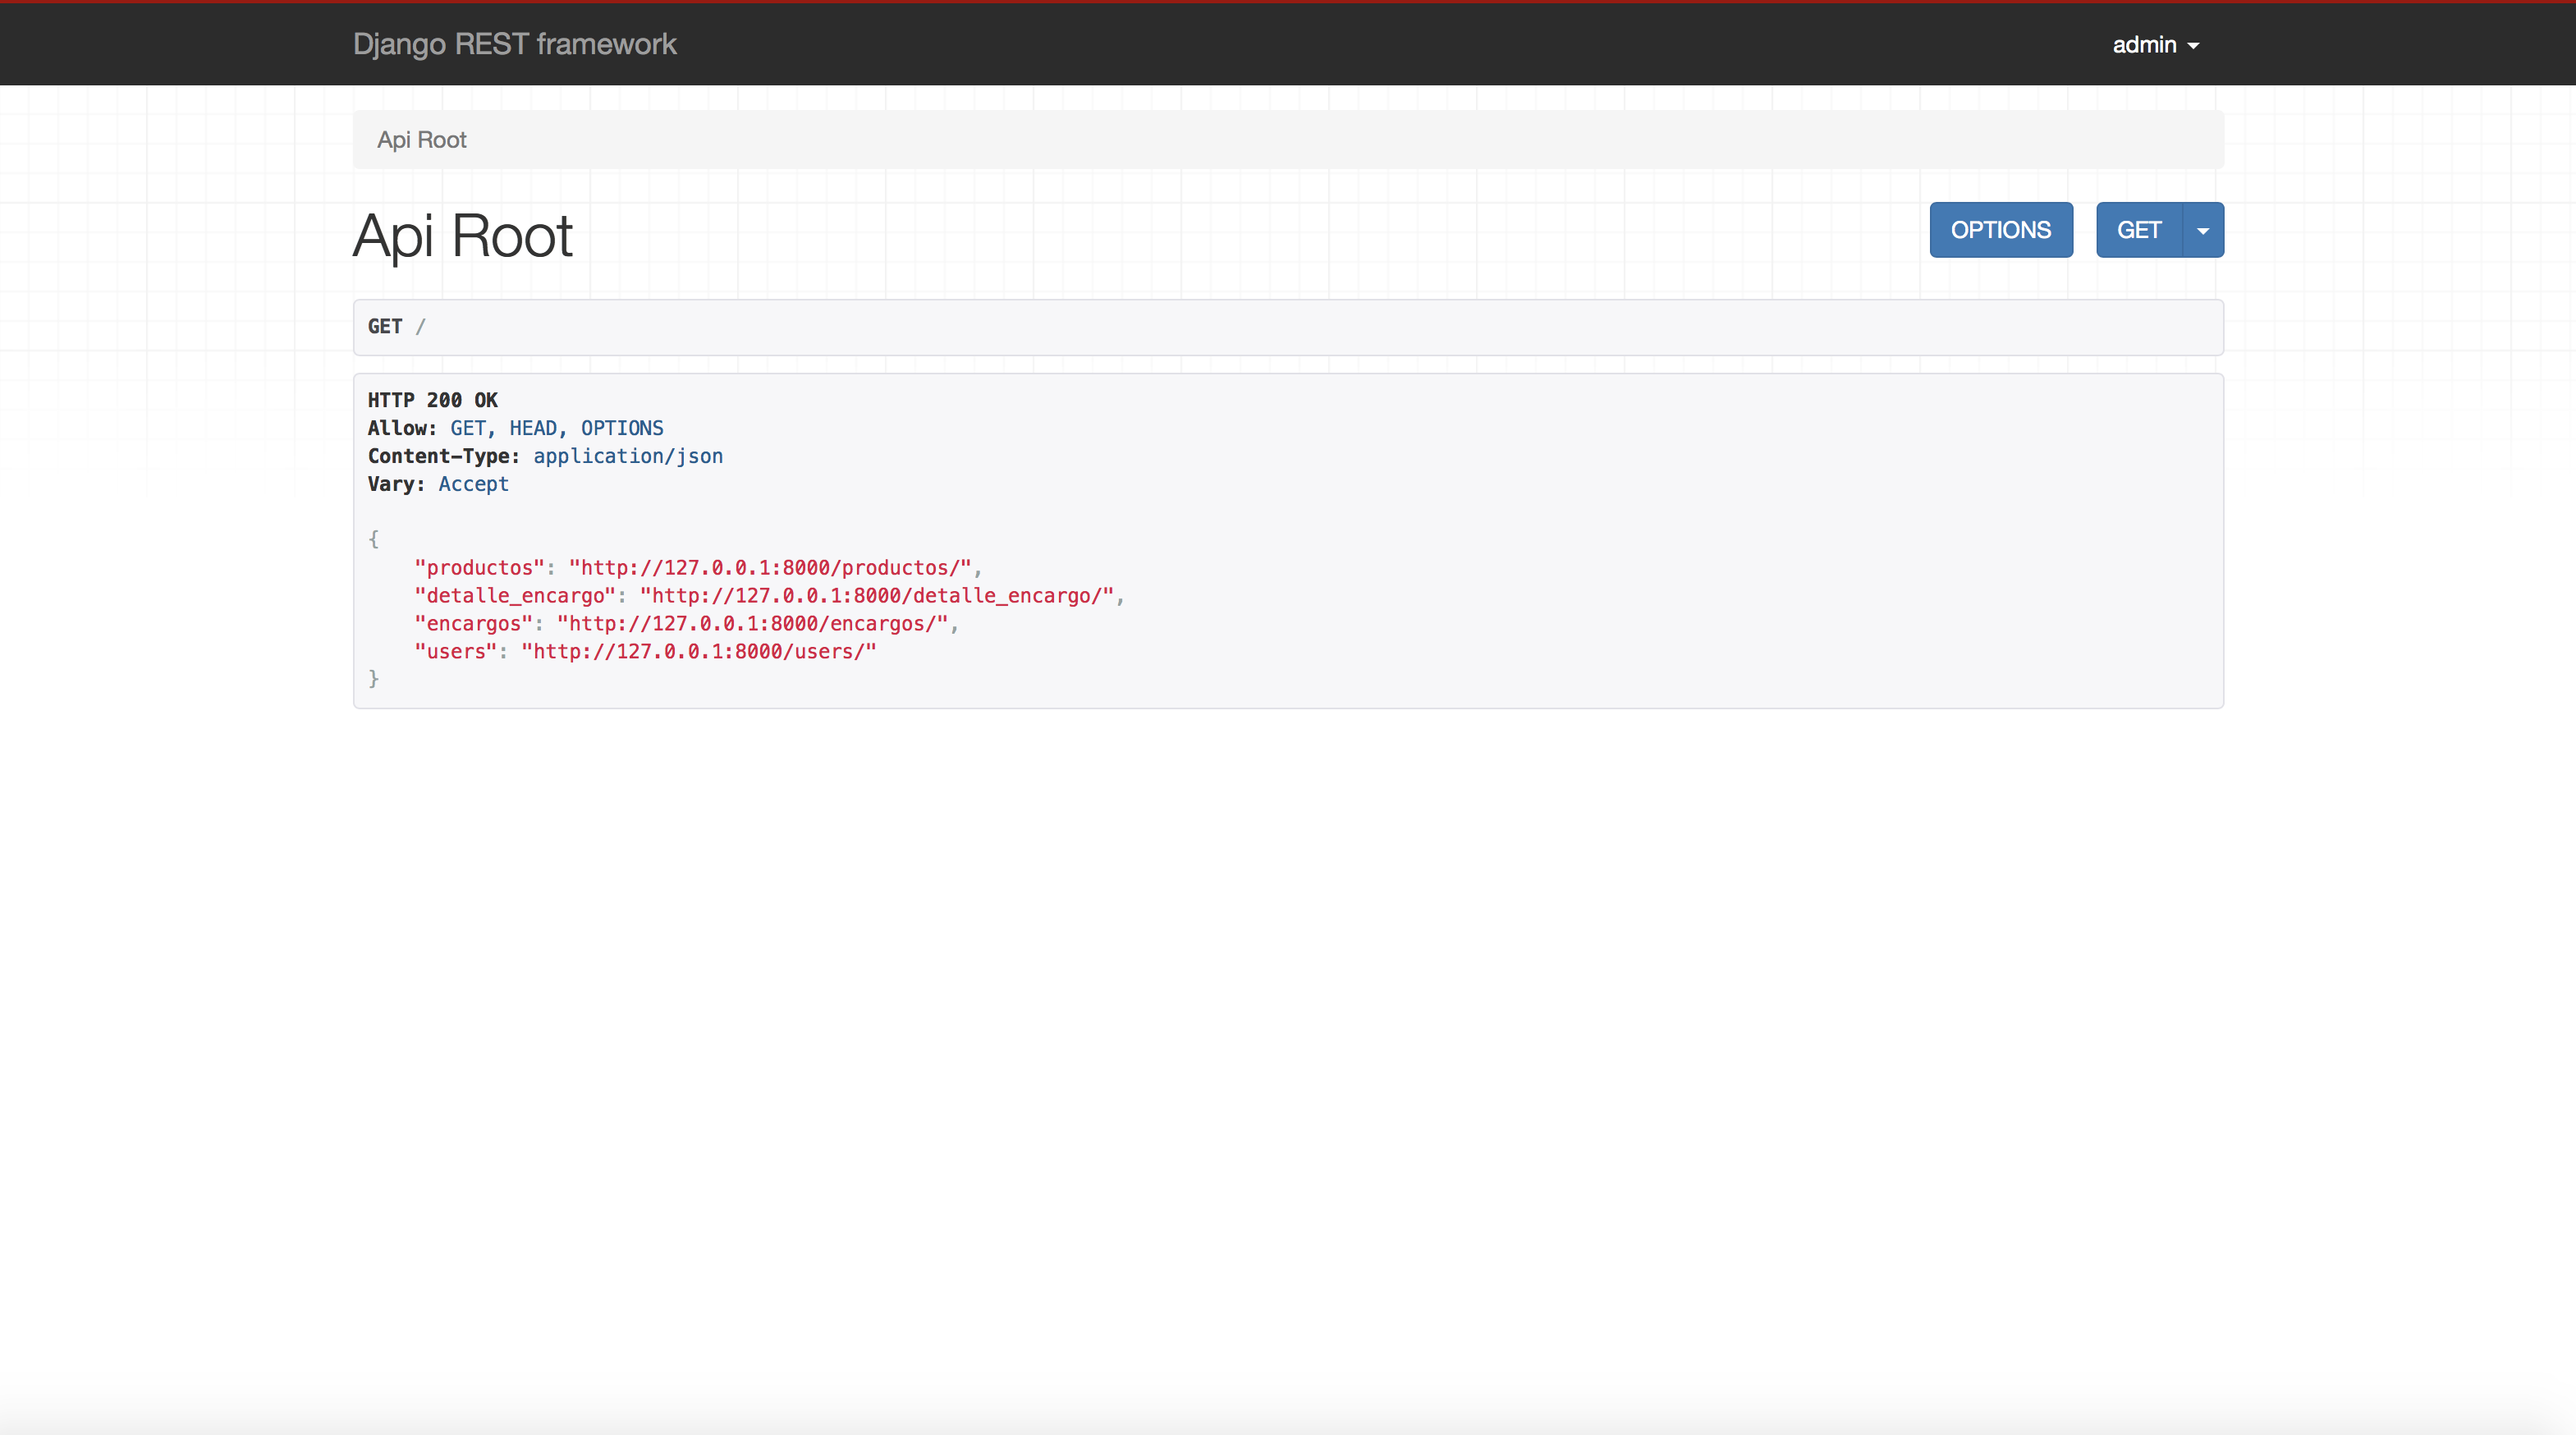
\includegraphics[width=12cm]{images/API_Root_Django.png}
	\end{center}
	\caption{Interfaz Django API RESTful}
	\label{fig:Encargo1}
\end{figure}

Conectarase a placa Arduino Mega 2560 á unha fonte de alimentación. Neste caso, conectarase vía USB. Unha vez conectado, terminal de operador inalámbrico vai mostrar que se conectou á rede inalámbrica asignada. Neste caso conectarase a \textit{HUAWEI-CW4a}.

\begin{figure}[H]
	\begin{center}
		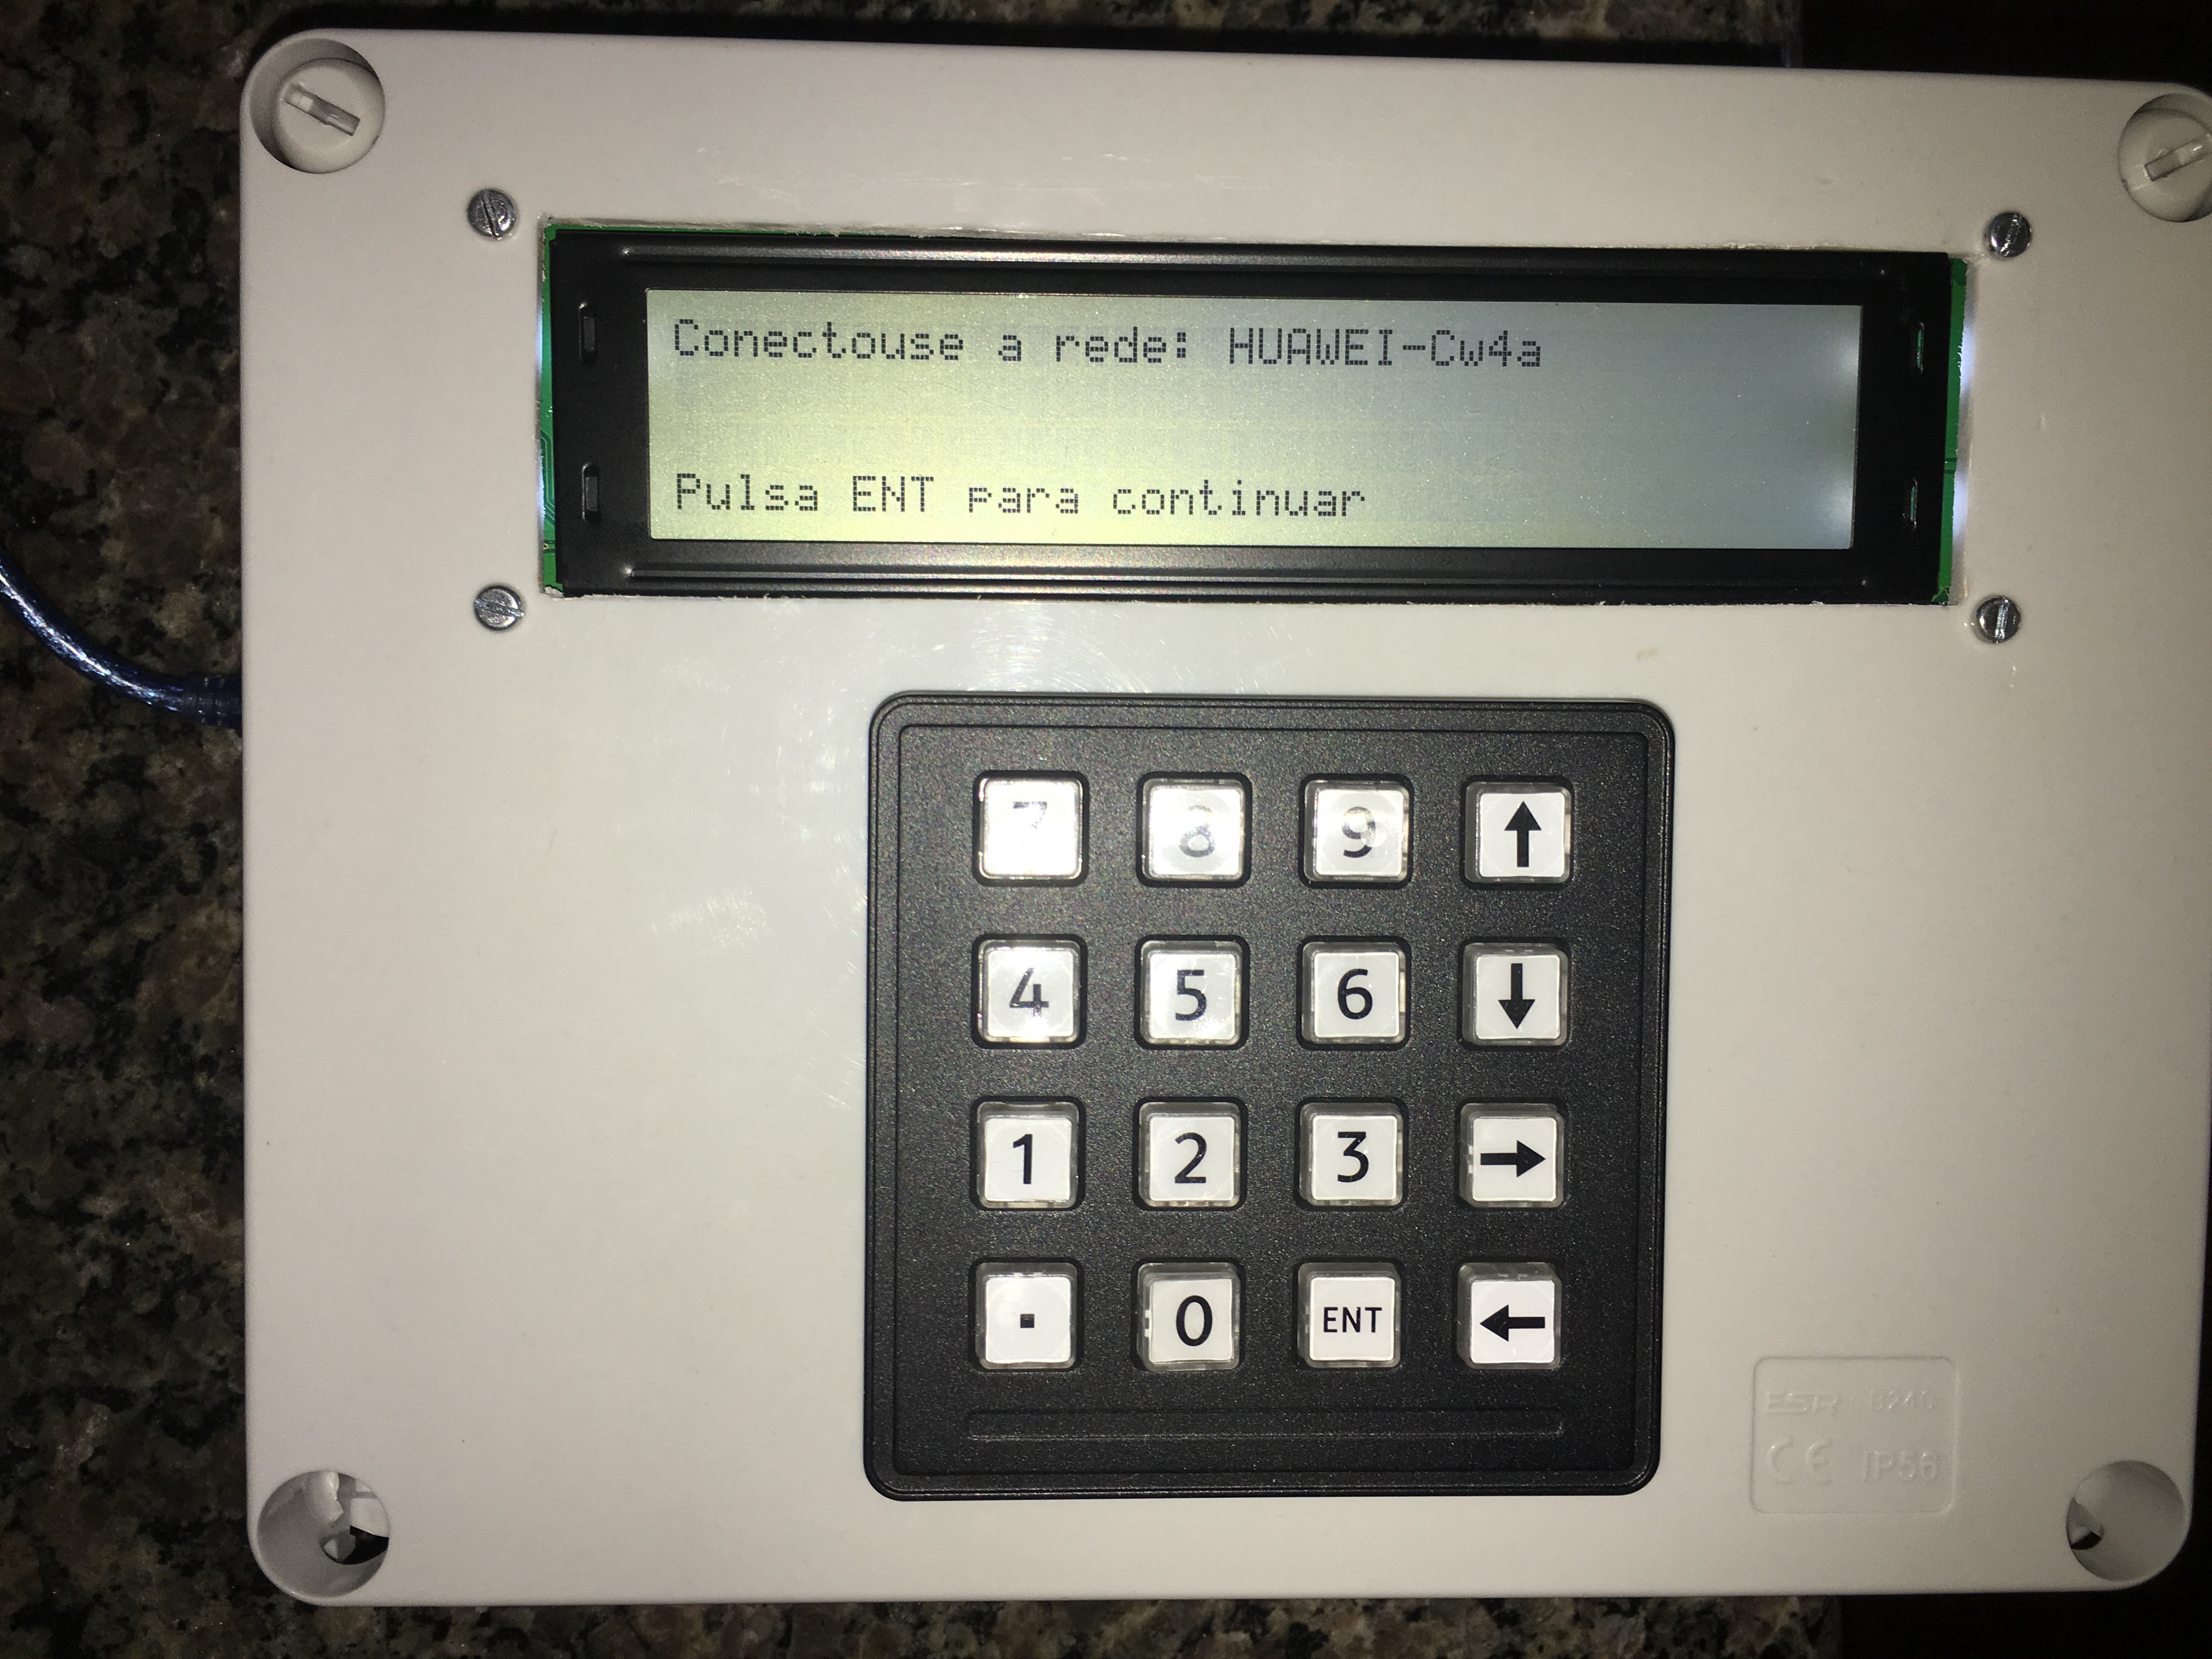
\includegraphics[width=10cm]{images/conectar_rede.JPG}
	\end{center}
	\caption{Conexión á rede HUAWEI-Cw4a}
	\label{fig:Encargo1}
\end{figure}

O terminal de operador mostra se hai encargos para facer. Neste caso, vai reflexar o encargo con id 2, xa que como podemos ver, o encargo con id 1 está completado.

\begin{figure}[H]
	\begin{center}
		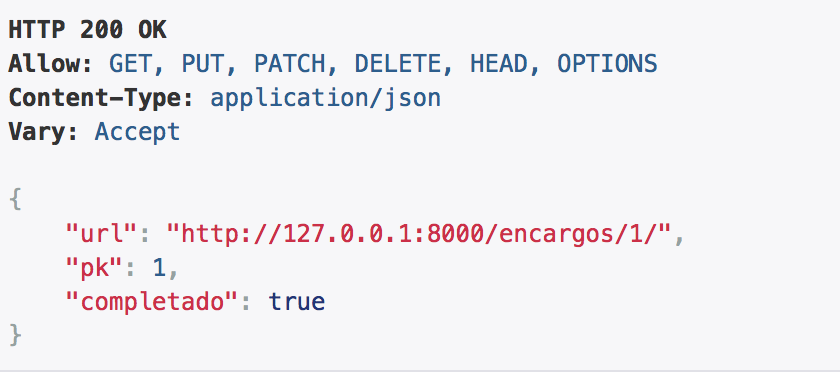
\includegraphics[width=8cm]{images/encargo_1.png}
	\end{center}
	\caption{Encargo con pk = 1}
	\label{fig:Encargo1}
\end{figure}

\begin{figure}[H]
	\begin{center}
		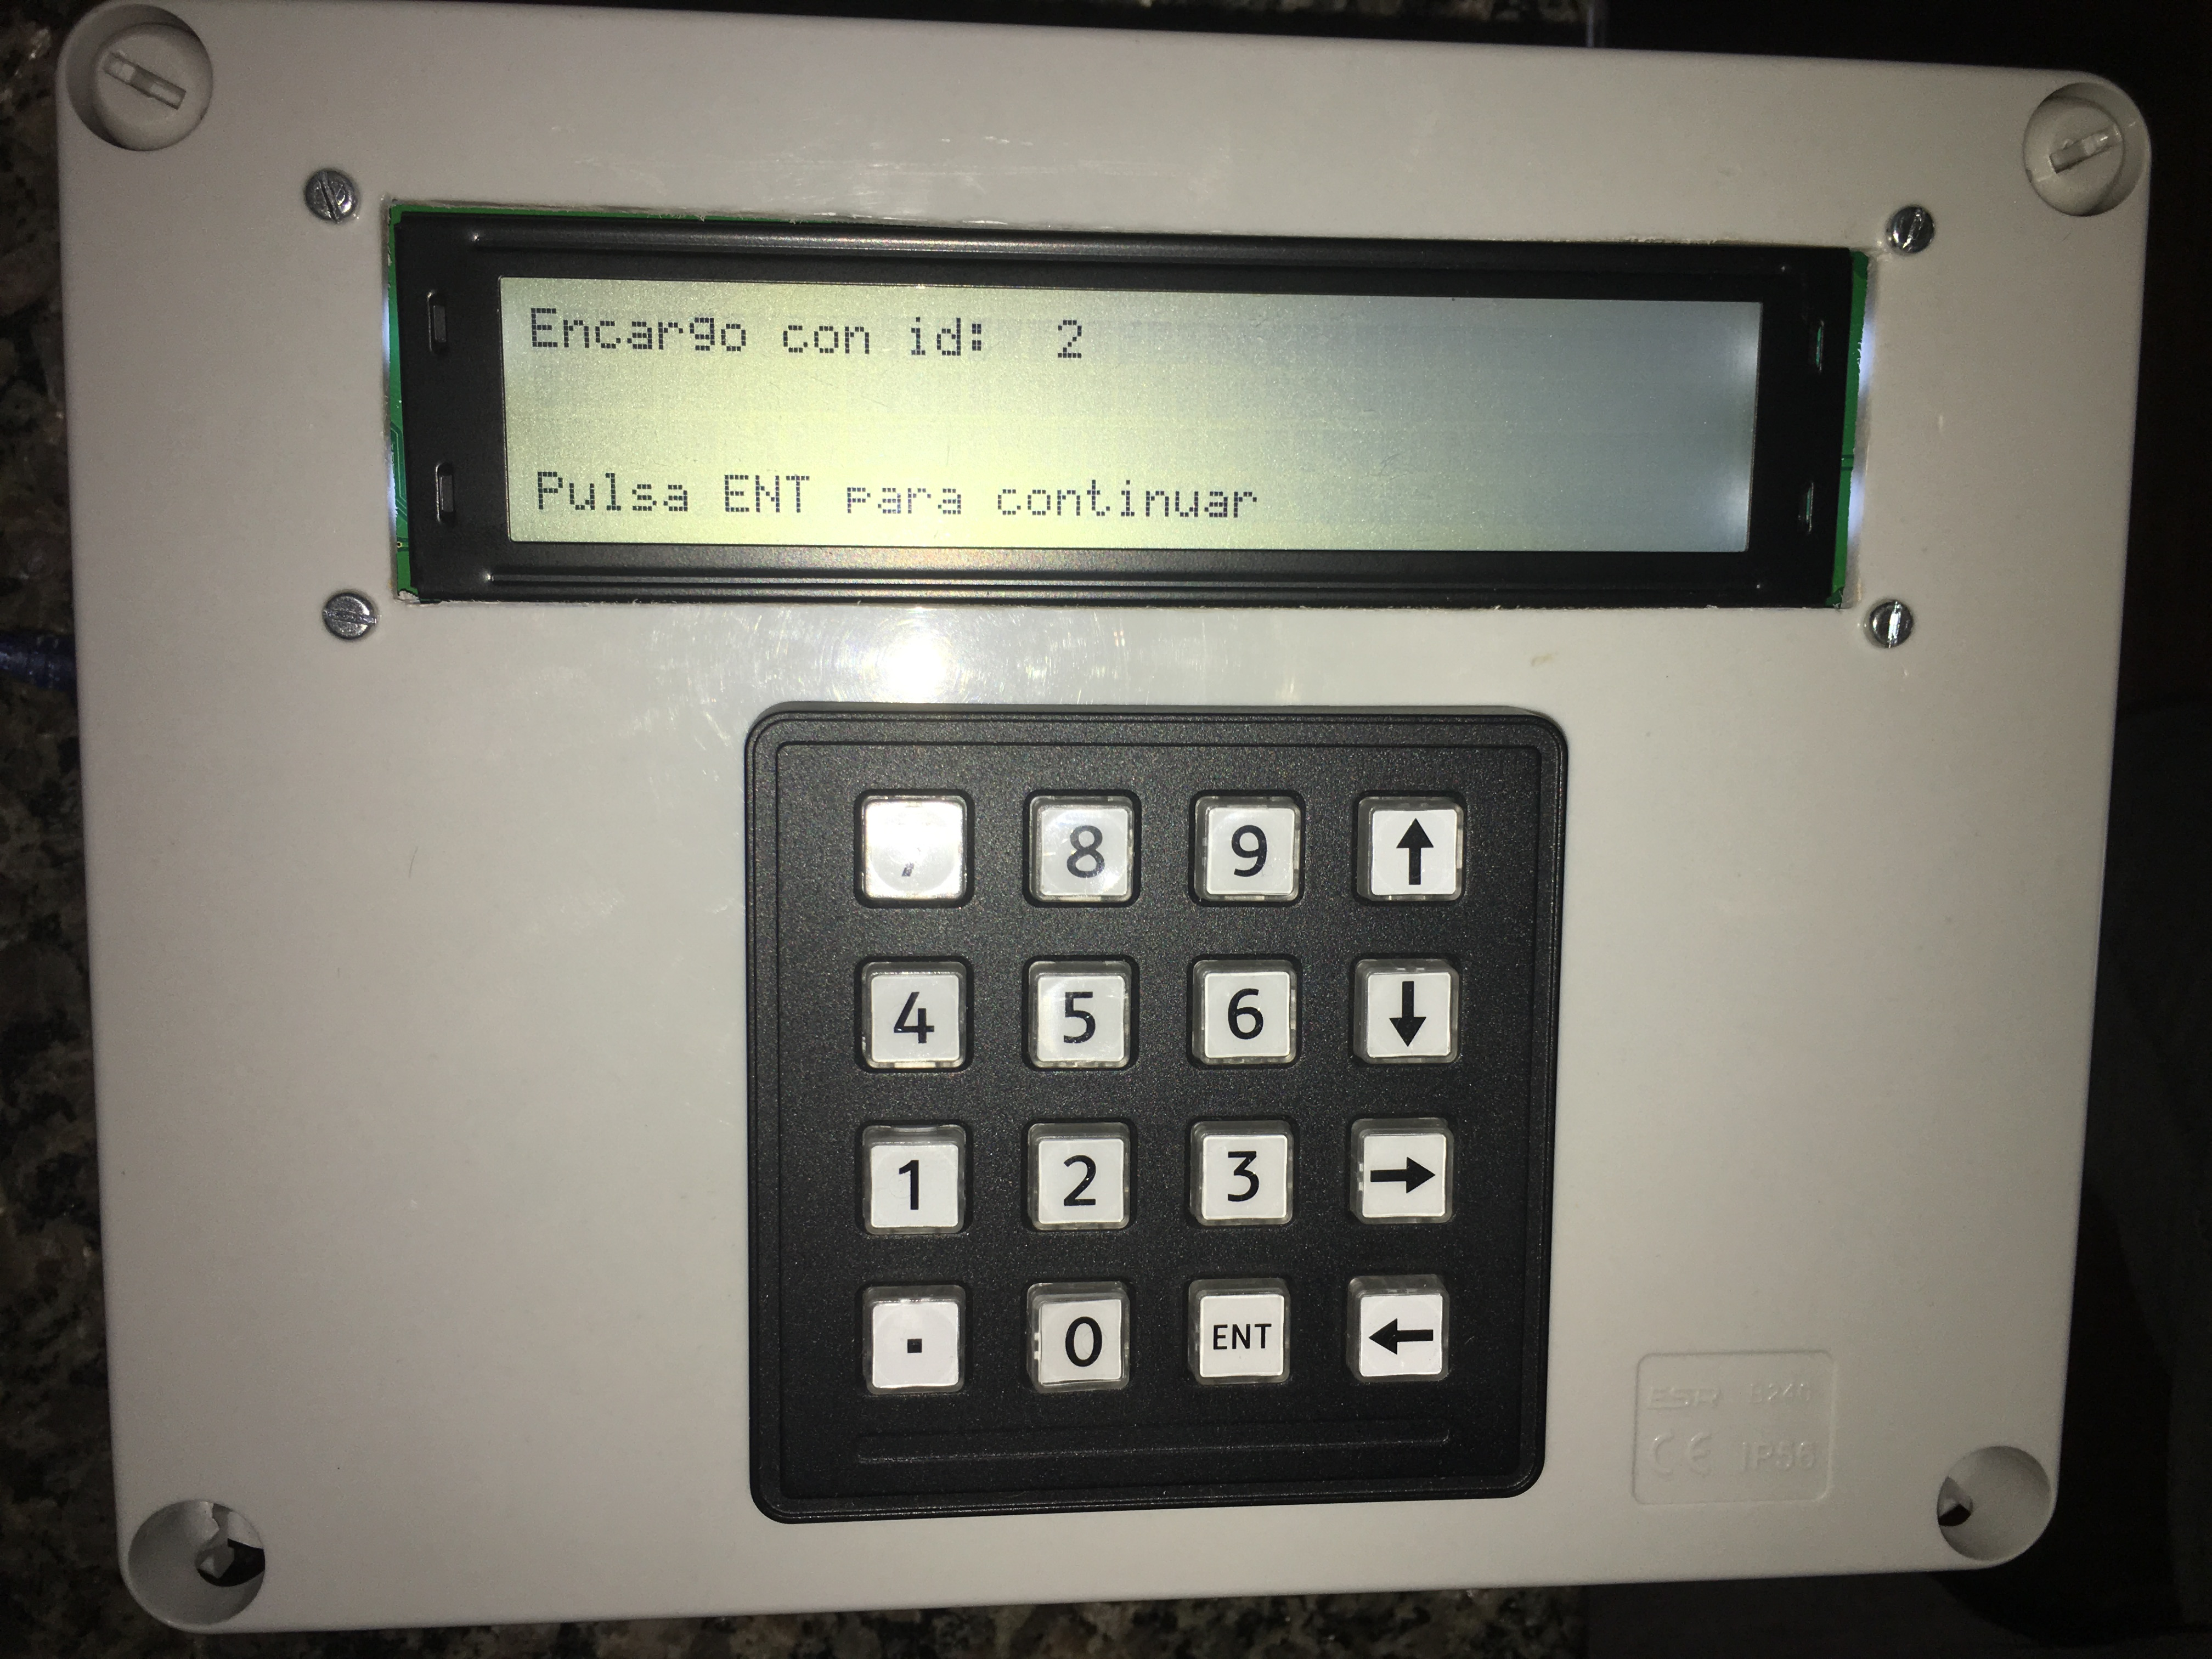
\includegraphics[width=10cm]{images/id_encargo.JPG}
	\end{center}
	\caption{Encargo pk = 2 no terminal}
	\label{fig:Encargo1}
\end{figure}

Ó darlle o operador a tecla ENT, o terminal mostrará o primeiro producto co seu nome, localización e cantidade. 

\begin{figure}[H]
	\begin{center}
		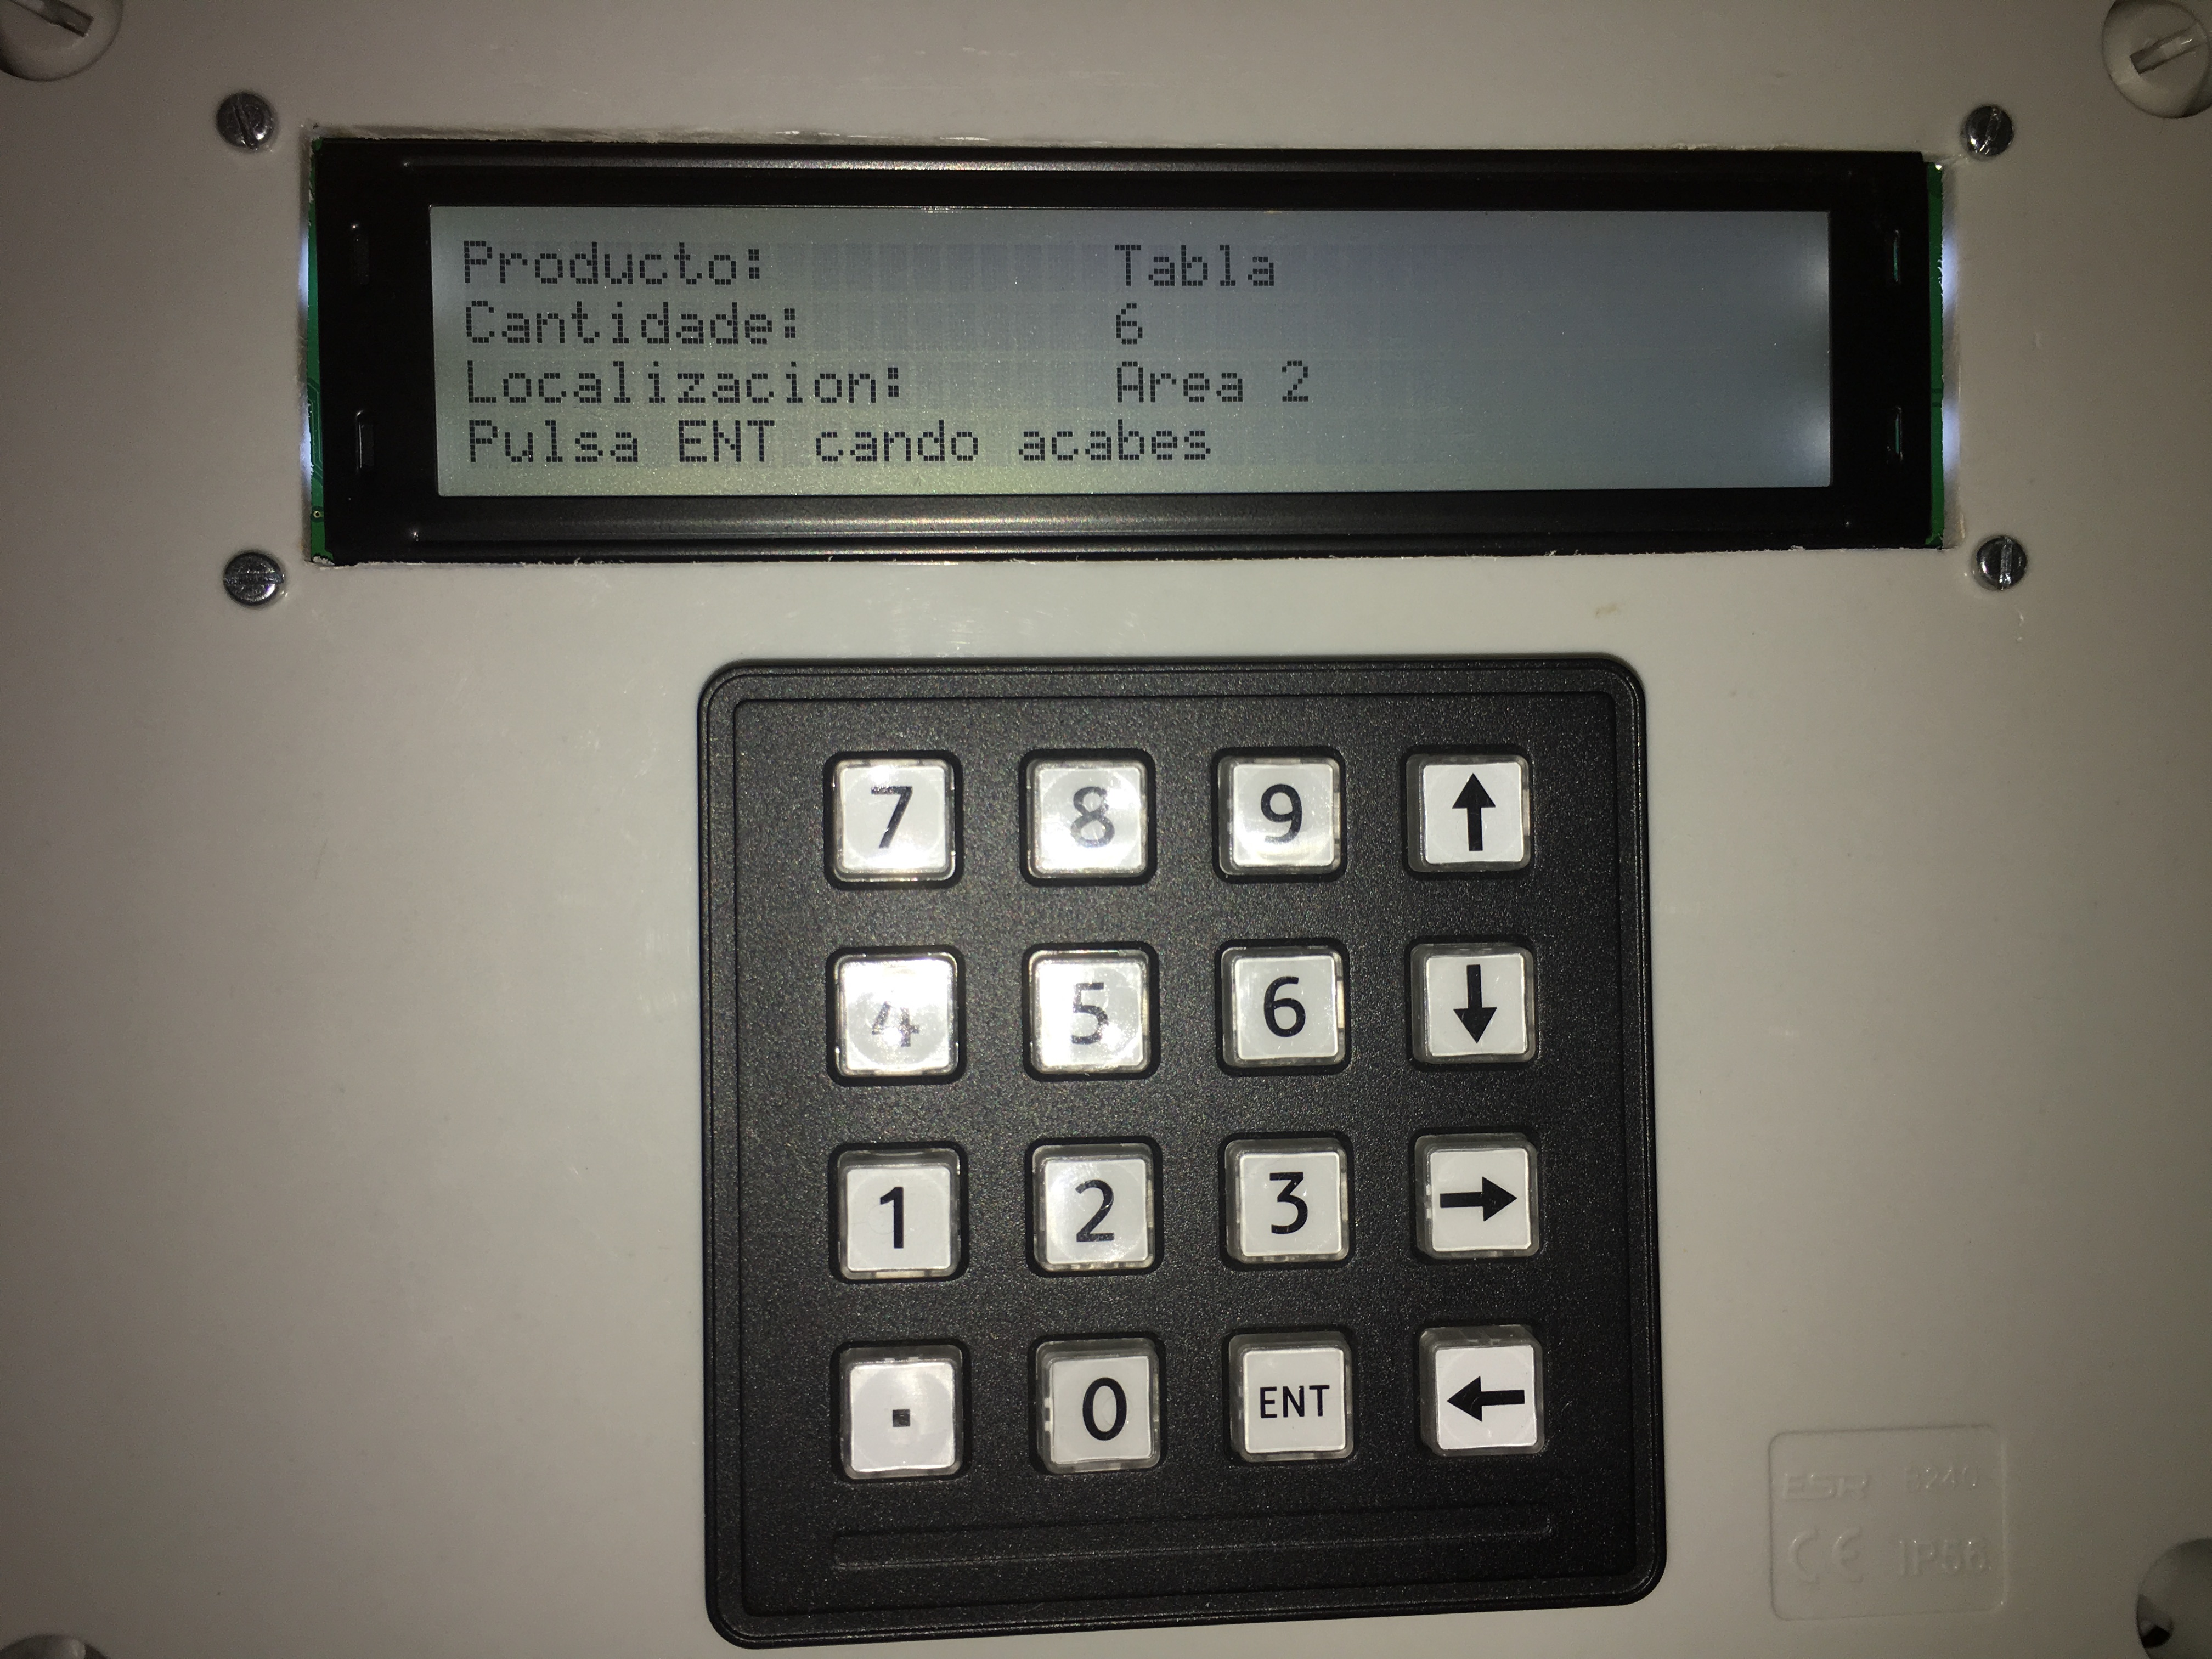
\includegraphics[width=10cm]{images/detalles_producto.JPG}
	\end{center}
	\caption{Detalles Producto}
	\label{fig:Encargo1}
\end{figure}

Cando o operador meta ese producto ou productos na caixa e lle de a tecla ENT, o terminal mostrará o seguinte producto e así sucesivamente.

Cando se complete o pedido, o terminal mostrará unha mensaxe na pantalla de que se rematou, quedando rexistrado no servidor.
\begin{figure}[H]
	\begin{center}
		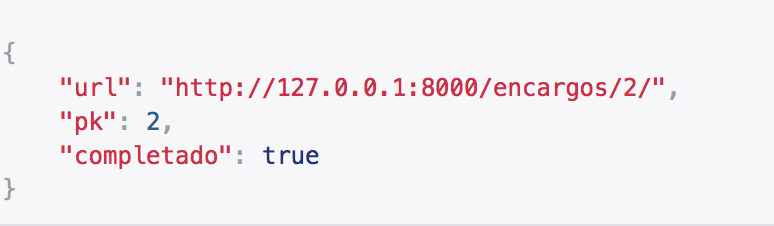
\includegraphics[width=8cm]{images/API_modificada.png}
	\end{center}
	\caption{Producto completado na aplicación}
	\label{fig:Encargo1}
\end{figure}
\begin{figure}[H]
	\begin{center}
		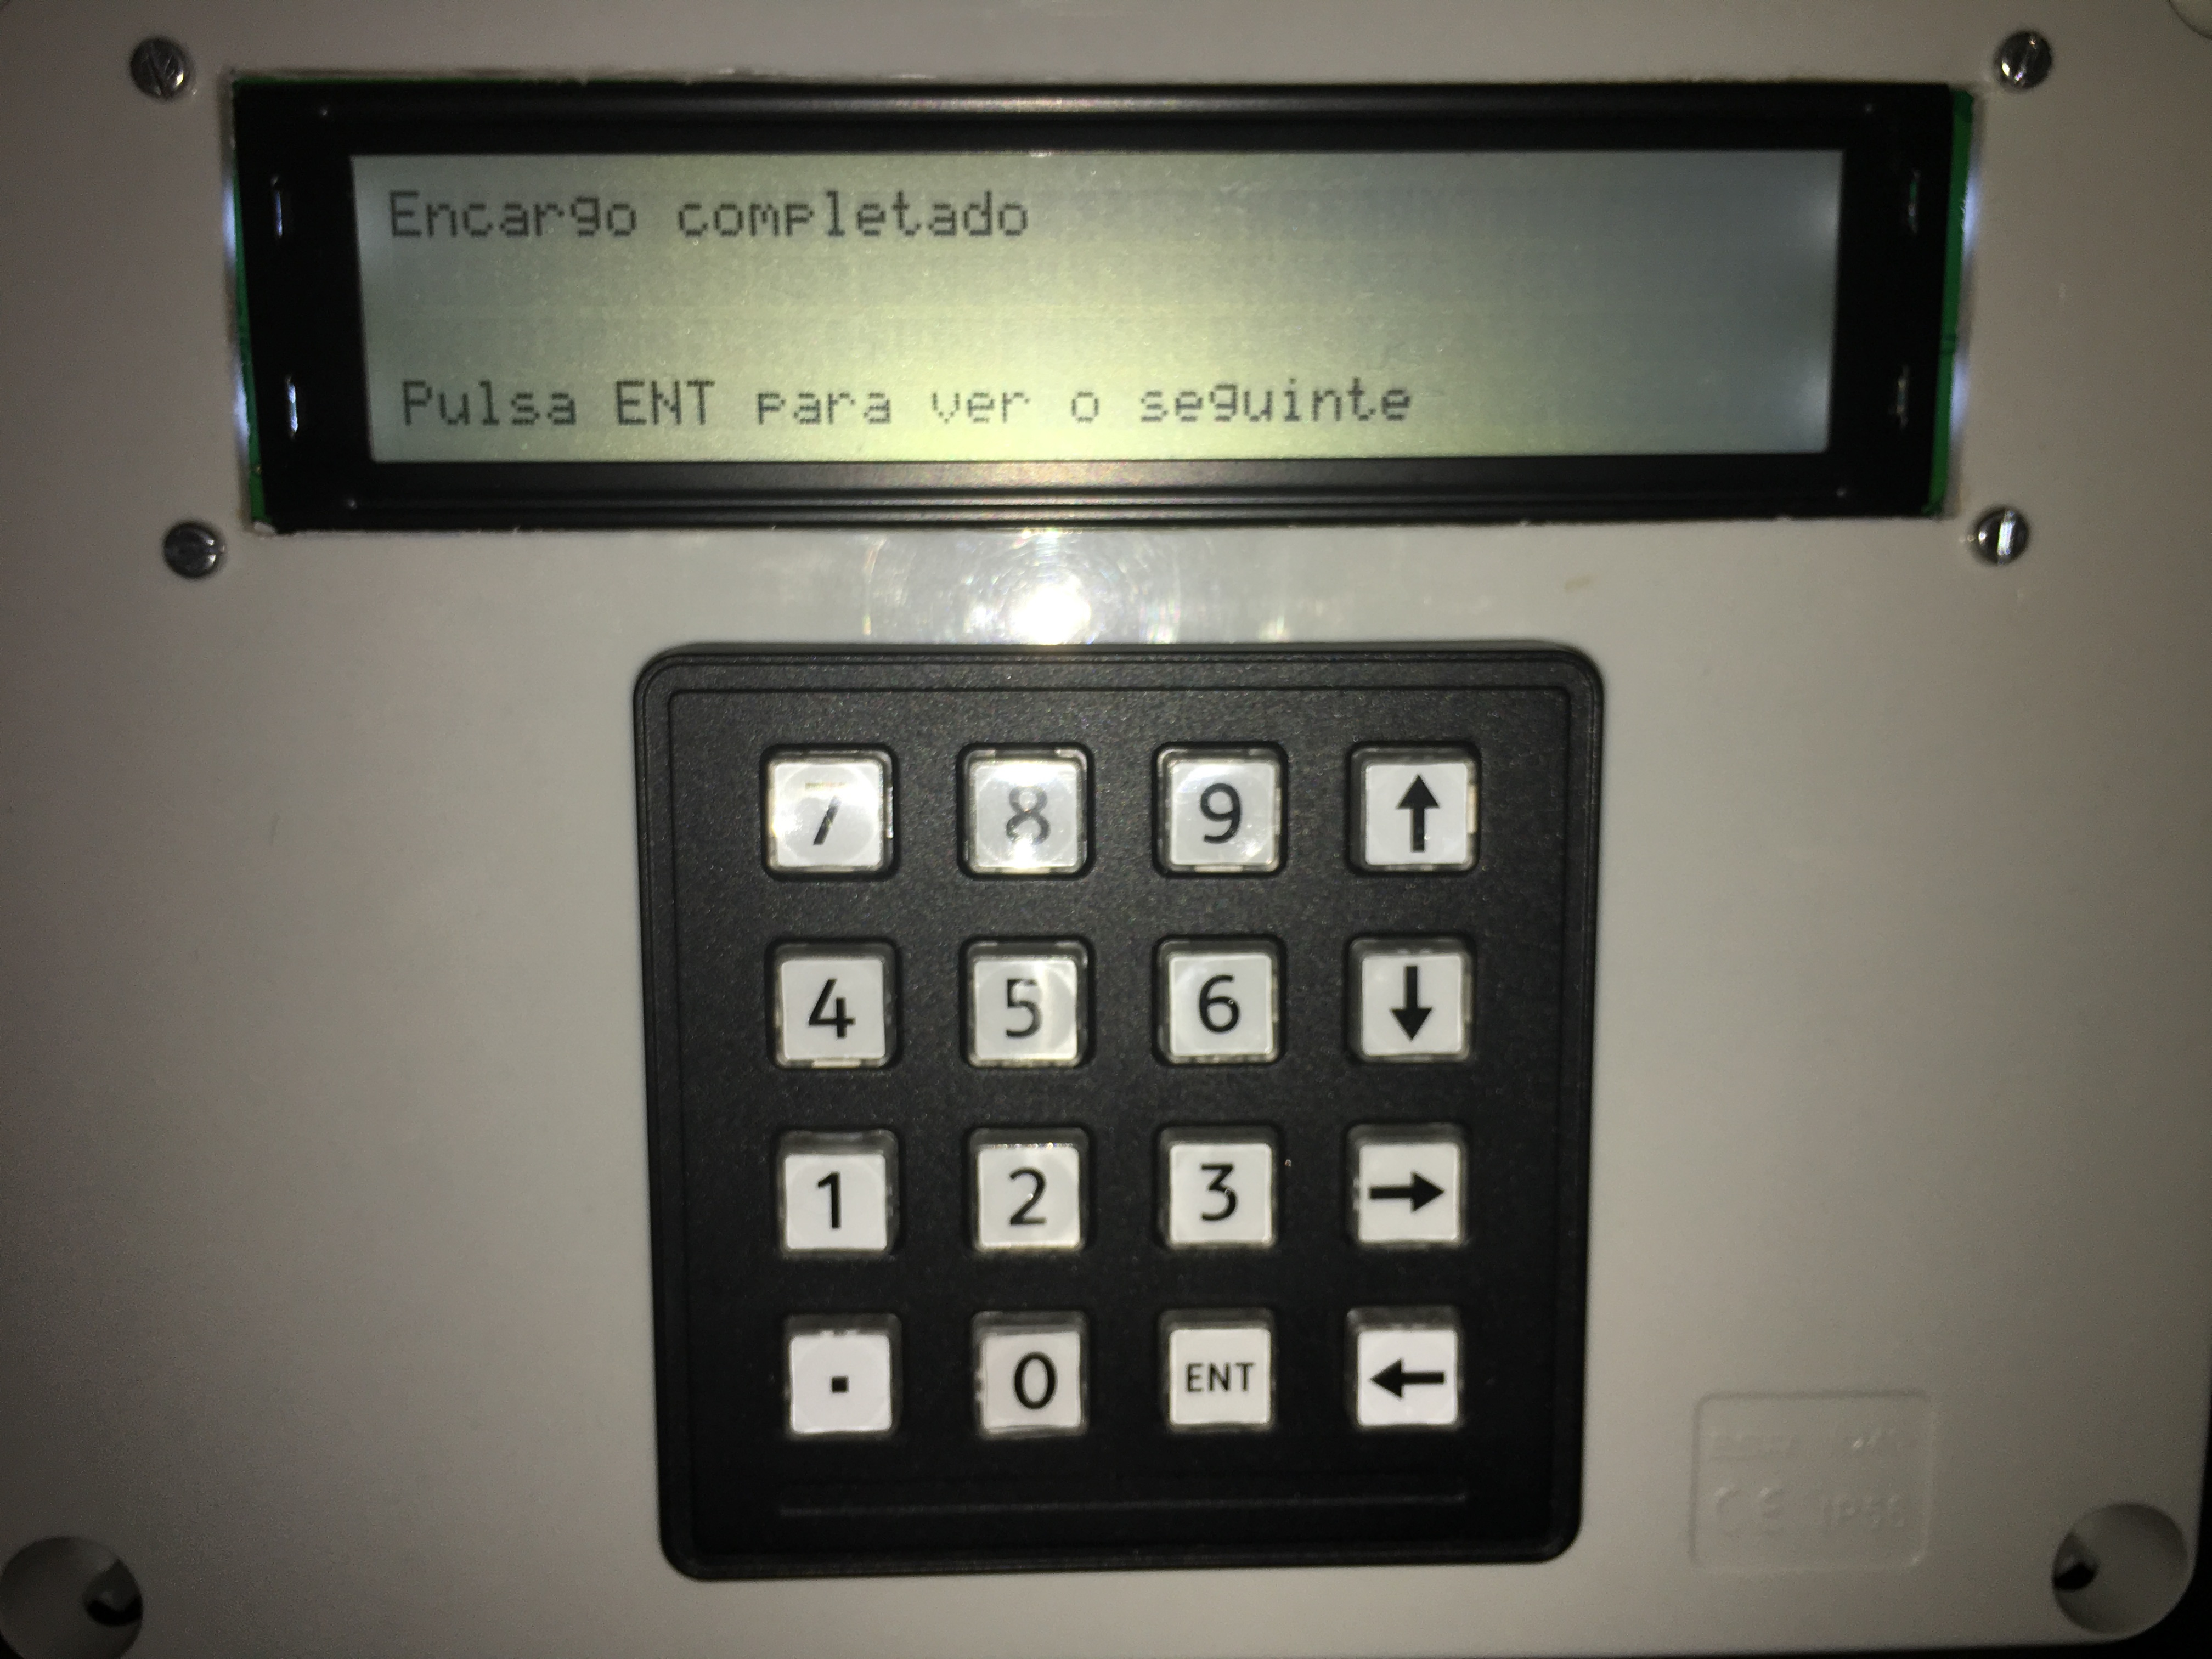
\includegraphics[width=10cm]{images/encargo_completado.JPG}
	\end{center}
	\caption{Producto completado no terminal}
	\label{fig:Encargo1}
\end{figure}

\chapter{Liñas futuras}

Para futuras versións deste proxecto, contémplanse as seguintes melloras:

\begin{itemize}
    \item Mellora da interfaz do servicio web, podendo subir fotos dos productos. Poderíase implementar con Bootstrap.
    \item Autentificación do operador mediante uso dun módulo que reconoza as huellas dactilares ou por un código específico para cada operador.
    \item Realización dunha PCB propia a partir dun microprocesador.
\end{itemize}


\begin{thebibliography}{99}

\bibitem{IoT} \textsc{Brian Russell, Drew Van Duren}; \emph{Practical Internet of Things Security}, PACKT Publishing (Xuño 2016).
\bibitem{Arduino} \textsc{Michael Margolis}, \emph{Arduino Cookbook}, O'Reilly.
\bibitem{Arduino2} \textsc{Harold Timmis}, \emph{Practical Arduino Engineering}, Apress.
\bibitem{Arduino3} \textsc{Marco Schwartz} \emph{Arduino Networking}, PACKT Publishing.
\bibitem{Django} \textsc{Gastón C. Hillar}, \emph{Building RESTful Python Web}, PACKT Publishing (Outubro 2016).
\bibitem{wArduino} \textit{Arduino} Dispoñible en \url{https://www.arduino.cc/}
\bibitem{DjangoDoc}\textit{Django Documentacion} Dispoñible en \url{https://docs.djangoproject.com/en/2.0/}
\bibitem{pantalla} \textit{DataSheet Pantalla Midas} Dispoñible en \url{http://www.farnell.com/datasheets/2021758.pdf?_ga=2.100621273.679229976.1530544951-2134847656.1521016684}
\bibitem{teclado} \textit{KeyPad STORM 720TFX SERIES} Dispoñible en \url{http://www.storm-interface.com/storm-720tfx-series-16-button.html}
\bibitem{ESP} \textit{ESP8266 Wiki}. Dispoñible en: \url{http://www.electrodragon.com/w/Category:ESP8266}
\bibitem{ESP2} \textit{Guía para configurar un ESP-01}. Dispoñible en: \url{https://programarfacil.com/podcast/como-configurar-esp01-wifi-esp8266/} 
\bibitem{WiFiEsp} \textit{WifiEsp Library}, A ESP8266 Library for Arduino. Dispoñible en: \url{https://github.com/bportaluri/WiFiEsp}.
\bibitem{Json} \textit{Arduino JSON}, A JSON Library for Arduino. Dispoñible en: \url{https://arduinojson.org}.

					
\end{thebibliography}

\stopcontents[parts]

\cleardoublepage
%%%%%%%%%%%%%%%%%%%%%%%%%%%%%%%%%%%%%%%%%%%%%%%%%%%%%%%%%%%%%%%%%%%%%%%%%%%%%%%%%%%%%%%%%%%%%%%%%%%%%%%%%%%%%%%%%%%%%%%%%%%%%%%%%%%%%%%%%%%%%%%%%%%%%%%%%%%%%%%%%%%%%%%%%%%%%
%%%%%%%%%%%%%%%%%%%%%%%%%%%%%%%%%%%%%%%%%%%%%%%%%%%%%%%%%%%%%%%%%%%%%%%%%%%%%%%%%%%%%%%%%%%%%%%%%%%%%%%%%%%%%%%%%%%%%%%%%%%%%%%%%%%%%%%%%%%%%%%%%%%%%%%
% DOCUMENTO ANEXOS
\renewcommand{\documento}{ANEXOS}
\begin{tikzpicture}[remember picture, overlay]
  \draw[line width = 0.5pt] ($(current page.north west) + (-20pt,-800.5pt)$) rectangle ($(current page.south east) + (-133.5pt,-722.5pt)$);
\end{tikzpicture}

\begin{center}
\begin{figure}[htbp]
\begin{center}

\includegraphics[angle=0, height=3.8cm]{images/EEILogo.png}
\end{center}
\end{figure}
\ \\
\begin{large}
\begin{center}
\color{blue}\textbf{Escola de Enxeñería Industrial}
\end{center}
\end{large}
\ \\
\ \\
\begin{large}
\begin{center}
\textbf{TRABALLO FIN DE GRAO}
\end{center}
\end{large}
\ \\
\ \\
\begin{large}
\begin{center}
{\titulouno}
\end{center}
\end{large}
\ \\
\ \\
\begin{normalsize}
\begin{center}
\textbf{\grado}
\end{center}
\end{normalsize}
\ \\
\ \\
\ \\
\ \\
\begin{normalsize}
\begin{center}
\textbf{Documento}
\end{center}
\end{normalsize}
\ \\
\begin{normalsize}
\begin{center}
\part{\bf{ANEXOS}}\thispagestyle{empty}
\end{center}
\end{normalsize}
\ \\
\ \\
\ \\
\ \\

\begin{center}
\begin{figure}[htbp]
\begin{center}

\includegraphics[angle=0, height=0.8cm]{images/UVIGOLogo.png}
\end{center}
\end{figure}
\end{center}

\end{center}

\cleardoublepage


\pagestyle{fancy}
%%%%%%%%%%%%%%%%%%%%%%%%%%%%%%%%%%%%%%%%%%%%%%%%%%%%%%%%%%%%%%%%%%%%%%%%%%%%%%%%%%%%%%%%%%%%
%%%%%%%%%%%%%%%%%%%%%%%%%%%%%%%%%%%%%%%%%%%%%%%%%%%%%%%%%%%%%%%%%%%%%%%%%%%%%%%%%%%%%%%%%%%%%%%%%%%%%%%%%%%%%%%%%%%%%%%%%%%%%%%%%%%%%%%%%%%%%%%%%%%%%%%%%%%%%%%%%%%%%%%%%%%%%
\addcontentsline{toc}{section}{Índice do documento Anexos}
\startcontents[parts]
\cleardoublepage

\begin{center}{\large \bf Índice de ANEXOS}\end{center}

{\hypersetup{hidelinks}\printcontents[parts]{}{-1}{\setcounter{tocdepth}{5}}}

\cleardoublepage
\chapter{Códigos de programación do Arduino}

\section{Librerías}

\subsection{PantallaMidas}

\subsubsection{Cabeceira}
\begin{lstlisting}
#ifndef PantallaMidas_h
#define PantallaMidas_h

#include <Arduino.h>

class PantallaMidas {
// Clase para o manexo dunha pantalla LCD alfanumérica de 4 filas e 40 columnas modelo
// Midas MC44005A6W-FPTLW desde unha placa Arduino. Configúrase un bus de datos de 4 bits. 

  private:  // Recursos privados a esta clase
  
    int _DB4, _DB5, _DB6, _DB7, _E1, _E2, _RS;
    // Número de señais Arduino usadas para a conexión á pantalla
    
    int _fila;  
    // Última fila posicionada 1...4
    
    void enviaOrde1(unsigned char orde);
    // Envía una orde al controlador 1 de la pantalla
    
    void enviaOrde2(unsigned char orde);
    // Envía unha orde ó controlador 2 da pantalla
    
    void enviaOrde12(unsigned char orde);
    // Envía unha orde ós controladores 1 e 2 da pantalla
    
    void busDatos4Bits(unsigned char dato);
    // Establece un valor para o bus de datos, usando os 4 bits
    // menos significativos do parámetro
    
    void pulsoE1();
    // Pulso a nivel alto en señal E1 para transferencia co controlador 1
    
    void pulsoE2();
    // Pulso a nivel alto en señal E1 para transferencia co controlador 1

  public:  // Membros públicos desta clase
  
    PantallaMidas(int DB4, int DB5, int DB6, int DB7, int E1, int E2, int RS);
    // Constructor ó que se lle indica qué señales Arduino están conectadas ás 
    // señaies da pantalla
    
    void configura();
    // Método que hai que usar en setup() para configurar e inicializar os 
    // controladores da pantalla
    
    void borra();
    // Borra toda a información mostrada na pantalla
    
    void posiciona(int fila, int columna);
    // Posiciona o cursor na fila (1...4) e columna (1...40)
    
    void escribeCadea(const char * cadea);
    // Escribe unha cadea de caracteres na posición actual do cursor

    void escribeCadea(const String cadea);
    
    void escribeCaracter(char caracter);
    // Escribe un carácter na posición actual do cursor

    void mostraCursor(int mostrao);
    // Fai que o cursor sea visible en función do buleano que se pasa por parámetro

};

#endif
\end{lstlisting}

\subsubsection{Código}

\begin{lstlisting}
#include <PantallaMidas.h>

PantallaMidas::PantallaMidas(int DB4, int DB5, int DB6, int DB7, int E1, int E2, int RS) {  
// Constructor ó que se lle indica que señaies Arduino están conectadas ás 
// señais da pantalla

  _DB4 = DB4;
  _DB5 = DB5;
  _DB6 = DB6;
  _DB7 = DB7;
  _E1 = E1;
  _E2 = E2;
  _RS = RS;
  // Garda os parámetros en datos privados
  
  _fila = 1;  // A fila inicial é a primeira
}

void PantallaMidas::configura() {
// Método que hai que usar en setup() para configurar e inicializar os 
// controladores da pantalla

  pinMode(_DB4, OUTPUT);
  pinMode(_DB5, OUTPUT);
  pinMode(_DB6, OUTPUT);
  pinMode(_DB7, OUTPUT);
  pinMode(_E1, OUTPUT);
  pinMode(_E2, OUTPUT);
  pinMode(_RS, OUTPUT);
  // Configura todas as señaies como salidas dixitais

  digitalWrite(_E1, LOW);
  digitalWrite(_E2, LOW);
  digitalWrite(_RS, LOW);
  // Pon a nivel baixo todas estas señais

  // A continuación execútase a secuencia de inicialización de ambos controladores
  
  delay(20);  // Espera 20 ms

  busDatos4Bits(3);
  pulsoE1();
  pulsoE2();
  // Transfire a ambos controladores o valor 3 

  delay(5);  // Espera 5 ms

  busDatos4Bits(3);
  pulsoE1();
  pulsoE2();
  // Transfire a ambos controladores o valor 3 
  
  delay(1);  // Espera 1 ms

  busDatos4Bits(3);
  pulsoE1();
  pulsoE2();
  // Transfire a ambos controladores o valor 3 
  
  delay(1);  // Espera 1 ms
  
  busDatos4Bits(2);
  pulsoE1();
  pulsoE2();
  // Transfire a ambos controladores o valor 2 

  delay(1);  // Espera 1 ms

  enviaOrde12(0x2D);
  delay(1);
  //0000101101
  //0 0 0 0 1 DL N F - -
  // Function set: 
  // DL=0 establece bus de 4bits 
  // N=1 establece manejo de 2 filas
  // F=1 establece xogo de carácteres de 5x11 puntos
  
  enviaOrde12(0x08);
  delay(1);
  // Display off

  borra();
  delay(2);
  // Clear display
  
  enviaOrde12(0x06);
  delay(1);
  // 0 0 0 0 0 0 0 0 0 1 ID SH
  // Métese o modo de configuración: 
  // ID=1 para que o cursor se mova hacia a dereita
  // SH=0 para que non se desplaza a pantalla
  
  enviaOrde12(0x0C);  // Display on
  delay(1);
}


void PantallaMidas::mostraCursor(int mostrao) {
// Fai que o cursor sexa visible en función do buleano que se pasa por parámetro

  unsigned char orde1, orde2;
  
  if (mostrao) {  // Si hai que mostrarlo ...
    if (_fila < 3) {  // Se é para o controlador 1 ...
      orde1 = 0x0F;  // Muestra cursor en 1
      orde2 = 0x0C;  // Oculta cursor en 2
    } else {
      orde1 = 0x0C;  // Oculta cursor en 1
      orde2 = 0x0F;  // Muestra cursor en 2
    }
  } else {  // Si hay que ocultarlo ...
    orde1 = 0x0C;  // Oculta cursor en 1
    orde2 = 0x0C;  // Oculta cursor en 2
  }
  enviaOrde1(orde1);  // Envía a orde ó controlador 1
  enviaOrde2(orde2);  // Envía a orde ó controlador 2
}


void PantallaMidas::pulsoE1() {
// Pulso a nivel alto en señal E1 para transferencia co controlador 1

  digitalWrite(_E1, HIGH);
  digitalWrite(_E1, LOW);
}

void PantallaMidas::pulsoE2() {
// Pulso a nivel alto en señal E2 para transferencia co controlador 2

  digitalWrite(_E2, HIGH);
  digitalWrite(_E2, LOW);
}


void PantallaMidas::busDatos4Bits(unsigned char dato) {
// Establece un valor para o bus de datos, utilizando os 4 bits
// menos significativos do parámetro

  if (dato & 0x01)  // Se o bit 0 é un 1 ...
      digitalWrite(_DB4, HIGH);  // pon a señal _DB4 a nivel alto
      else digitalWrite(_DB4, LOW);  // senon, pon a señal _DB4 a nivel baixo
      
  if (dato & 0x02)  // Se o bit 1 é un 1 ...
      digitalWrite(_DB5, HIGH);  // pon a señal _DB5 a nivel alto
      else digitalWrite(_DB5, LOW);  // si no, pon la señal _DB5 a nivel baixo
      
  if (dato & 0x04)  // Se o bit 2 é un 1 ...
      digitalWrite(_DB6, HIGH);  // pon a señal _DB6 a nivel alto
      else digitalWrite(_DB6, LOW);  // senon, pon a señal _DB6 a nivel baixo
      
  if (dato & 0x08)  // Se o bit 3 é un 1 ...
      digitalWrite(_DB7, HIGH);  // pon a señal _DB7 a nivel alto
      else digitalWrite(_DB7, LOW);  // senon, pon la señal _DB7 a nivel baixo
}


void PantallaMidas::borra() {
// Borra toda a información mostrada na pantalla

  enviaOrde12(0x01); 
  // Envía a orde de código 0x01 ós dous controladores
  
  delay(2);  // Espera 2 ms a que se acabe de executar
}


void PantallaMidas::escribeCadea(const char * cadea) {
// Escribe unha cadea de caracteres na posición actual do cursor

  int i;  // Contador para o bucle
  
  i = 0;  // Desde o comezo do array...
  while(cadea[i])  // Mientras no se llegue a un byte con valor 0 ...
    escribeCaracter(cadea[i++]);  // Escribe o carácter e pasa ó seguinte
}

void PantallaMidas::escribeCadea(const String cadea) {
  //Escribe un array de strings na poisicion actual do cursor

  int i;

  i = 0;
  while(cadea[i])
    escribeCaracter(cadea[i++]);
}


void PantallaMidas::posiciona(int fila, int columna) {
// Posiciona o cursor na fila (1...4) e columna (1...40)

  int posicion;  // Posición na memoria interna do controlador

  if (fila < 3) {   // Si es para el primer controlador ...
    
    posicion = (fila - 1) * 0x40 + columna - 1;
    // A primiera posición comeza en 0 para a fila 1 e en 0x40 para a fila 2
    // Ó avanzar nas columnas, avánzase en memoria a posicións consecutivas
    
    enviaOrde1(0x80 | posicion);
    // Envía unha orde ó controlador 1 coa nova posición do cursor
    
  } else {  // O mesmo para o controlador 2
    posicion = (fila - 3) * 0x40 + columna - 1;
    enviaOrde2(0x80 | posicion);
  }
  
  delay(1);  // Espera 1 ms a que o cursor se posicione
  _fila = fila;  // Recorda a fila onde está situado o cursor
}


void PantallaMidas::enviaOrde1(unsigned char orde) {
// Envía unha orde ó controlador 1 da pantalla

  digitalWrite(_RS, LOW);  // Pon a señal RS a nivel baixo
  
  busDatos4Bits(orde >> 4);  // Pon os 4 bits máis significativos no bus de datos
  pulsoE1();  // Pulso en E1 para transferir esos bits
  busDatos4Bits(orde & 0x0F);  // Pon os 4 bits menos significativos no bus de datos
  pulsoE1();  // Pulso en E1 para transferir esos bits
}


void PantallaMidas::enviaOrde2(unsigned char orde) {
// Envía unha orde ó controlador 2 da pantalla

  digitalWrite(_RS, LOW);  // Pon a señal RS a nivel baixo
  
  busDatos4Bits(orde >> 4);  // Pon os 4 bits máis significativos no bus de datos
  pulsoE2();  // Pulso en E2 para transferir esos bits
  busDatos4Bits(orde & 0x0F);  // Pon os 4 bits menos significativos no bus de datos
  pulsoE2();  // Pulso en E2 para transferir esos bits
}


void PantallaMidas::enviaOrde12(unsigned char orde) {
// Envía una orde a ambos controladores

  enviaOrde1(orde);   // Envía a orde ó controlador 1
  enviaOrde2(orde);   // Envía a orde ó controlador 2
}


void PantallaMidas::escribeCaracter(char caracter) {
// Envía un carácter á pantalla, que se mostrará na posición actual do cursor. 
// A posición do cursor increméntase

  digitalWrite(_RS, HIGH);   // Pon a señal RS a nivel alto
  
  busDatos4Bits(caracter >> 4);  // Pon os 4 bits máis significativos no bus de datos
  if (_fila < 3)  // Se é para o controlador 1 ...
    pulsoE1();   // pulso en E1 para transferir esos bits ó controlador 1
    else pulsoE2();  // se non, pulso en E2 para transferir esos bits ó controlador 2
    
  busDatos4Bits(caracter & 0x0F);    // Pon os 4 bits menos significativos no bus de datos
  if (_fila < 3)  // Se é para o controlador 1 ...
    pulsoE1();   // pulso en E1 para transferir esos bits ó controlador 1
    else pulsoE2();  // senon, pulso en E2 para transferir esos bits ó controlador 2
    
  delay(1);  // Retardo de 1 ms para esperar a que se escriba o carácter
}
\end{lstlisting}

\subsection{Teclado 4x4}

\subsubsection{Cabeceira}

\begin{lstlisting}
#ifndef Teclado4x4_h
#define Teclado4x4_h

class Teclado4x4 {
  private:
    int _salidasFilas[4], * _entradasColumnas[4];
    char _caracteres[17];
    int _pulsado, _fila, _columna;
    unsigned long _t;
  public:
    Teclado4x4(int F1, int F2, int F3, int F4, int C1, int C2, int C3, int C4, char *caracteres);
    void configura();
    int comproba();
};

#endif
\end{lstlisting}

\subsubsection{Codigo}
\begin{lstlisting}
#include <Teclado4x4.h>
#include <Arduino.h>

Teclado4x4::Teclado4x4(int F1, int F2, int F3, int F4, int C1, int C2, int C3, int C4, char *caracteres) {
  _salidasFilas[0] = F1;
  _salidasFilas[1] = F2;
  _salidasFilas[2] = F3;
  _salidasFilas[3] = F4;
  _entradasColumnas[0] = C1;
  _entradasColumnas[1] = C2;
  _entradasColumnas[2] = C3;
  _entradasColumnas[3] = C4;
  strcpy(_caracteres,caracteres);
  // Garda os parámetros en datos privados
}


void Teclado4x4::configura() {
  int i;
  //memcpy (_salidasFilas, salidasFilas, 4 * sizeof(int));
  //memcpy (_entradasColumnas, entradasColumnas, 4 * sizeof(int));
  //strcpy (_caracteres, caracteres);
  for (i = 0; i < 4; i++)
    pinMode(_entradasColumnas[i], INPUT_PULLUP);
  _pulsado = 0;
  _t = millis();
}


int Teclado4x4::comproba () {
  int iSalida, iEntrada;

  if (millis() - _t < 10) 
    return 0;
    else _t = millis();

  if (_pulsado) {
    pinMode(_salidasFilas[_fila], OUTPUT);
    digitalWrite(_salidasFilas[_fila], LOW);
    _pulsado = digitalRead(_entradasColumnas[_columna]) == LOW;
    pinMode(_salidasFilas[_fila], INPUT);    
    if (_pulsado)
      return 0;
  }
  
  if (! _pulsado) {
    for (iSalida = 0; iSalida < 4 && ! _pulsado; iSalida ++) {
      pinMode(_salidasFilas[iSalida], OUTPUT);
      digitalWrite(_salidasFilas[iSalida], LOW);
      for (iEntrada = 0; iEntrada < 4 && ! _pulsado; iEntrada ++) {
        if (digitalRead(_entradasColumnas[iEntrada]) == LOW) {
          _pulsado = 1;
          _fila = iSalida;
          _columna = iEntrada;
        }
      }
      pinMode(_salidasFilas[iSalida], INPUT);
    }
  }
  
  if (_pulsado)
    return _caracteres[_fila * 4 + _columna];
  else return 0;
}
\end{lstlisting}

\subsection{Consola}
\subsubsection{Cabeceira}
\begin{lstlisting}
#ifndef CONSOLA_H_
#define CONSOLA_H_

#include "PantallaMidas.h"
#include "Teclado4x4.h"

class Consola {
  // Un obxecto de esta clase representa a unha consola composta por un teclado e unha pantalla
  
  private:
      PantallaMidas pantalla;
      Teclado4x4 teclado;
      // Cada obxecto Consola contén obxectos para manexar teclado e pantalla
      
      char _cadea[41];
      
  public: 
  
      Consola(int DB4, int DB5, int DB6, int DB7, int E1, int E2, int RS, int F1, int F2, int F3, int F4, int C1, int C2, int C3, int C4, char * caracteres);
      // Constructor ó que lle proporcionamos os datos necesarios para inicializar a pantalla e o teclado
      
      void configura();  // Utilizado no setup() para configurar estos dispositivos
      
      void visualizaEnteiro(int fila, int columna, unsigned int valor);
      void visualizaReal(int fila, int columna, float valor, int nCaracteres, int nDecimales);
      void visualizaCadea(int fila, int columna, char * cadea);  
      void visualizaCadea(int fila, int columna, String cadea);
      // Para visualizar información en pantalla
      
      char introduceCaracter();
      int introduceEnteiro(int fila, int columna, int nCaracteres);
      float introduceReal(int fila, int columna, int nCaracteres);
      void introduceCadea(int fila, int columna, char * validos, int nCaracteres, char * resultado);
      // Para introducir información por teclado
      
      void borraPantalla();
      // Para borrar a pantalla
};

#endif
\end{lstlisting}

\subsubsection{Código}
\begin{lstlisting}
#include "Consola.h"
#include <string.h>


Consola::Consola(int DB4, int DB5, int DB6, int DB7, int E1, int E2, int RS, int F1, int F2, int F3, int F4, int C1, int C2, int C3, int C4, char * caracteres):
    pantalla(DB4, DB5, DB6, DB7, E1, E2, RS),
    teclado(F1, F2, F3, F4, C1, C2, C3, C4, caracteres) {
}

void Consola::configura() {
  pantalla.configura();
  teclado.configura();
}

void Consola::visualizaEnteiro(int fila, int columna, unsigned int valor) {
  pantalla.posiciona(fila, columna);
  unsigned long aux = valor;
  sprintf(_cadea,"%ld",aux);
  pantalla.escribeCadea(_cadea);
}

void Consola::visualizaReal(int fila, int columna, float valor, int nCaracteres, int nDecimales) {
  pantalla.posiciona(fila, columna);
  dtostrf(valor, nCaracteres, nDecimales, _cadea);
  pantalla.escribeCadea(_cadea);
}

void Consola::visualizaCadea(int fila, int columna, char * cadea) {
  pantalla.posiciona(fila, columna);
  pantalla.escribeCadea(cadea);
}

void Consola::visualizaCadea(int fila, int columna, String cadea) {
  pantalla.posiciona(fila, columna);
  pantalla.escribeCadea(cadea);
}

char Consola::introduceCaracter() {
  char caracter;
  do {
    caracter = teclado.comproba();
  } while (caracter == 0);
  return caracter;
}

void Consola::introduceCadea(int fila, int columna, char * validos, int nCaracteres, char * resultado) {
  int i;
  char caracter;
  pantalla.posiciona(fila, columna);
  for (i = 0; i < nCaracteres; i++)
      pantalla.escribeCaracter(' ');
  pantalla.posiciona(fila, columna);
  pantalla.muestraCursor(true);
  i = 0;
  do {
      caracter = introduceCaracter();
      if (strchr(validos, caracter) != NULL && i < nCaracteres) {
          resultado[i] = caracter;
          i++;
          pantalla.escribeCaracter(caracter);
      }
      if (caracter == 'i') {
          i--;
          pantalla.posiciona(fila, columna+i);
          pantalla.escribeCaracter(' ');
          pantalla.posiciona(fila, columna+i);
      }
  } while (caracter != 'e');
  pantalla.muestraCursor(false);
  resultado[i] = 0;
}

int Consola::introduceEnteiro(int fila, int columna, int nCaracteres) {
  introduceCadea(fila, columna, "0123456789", nCaracteres, _cadea);
  return atoi(_cadea);
}

float Consola::introduceReal(int fila, int columna, int nCaracteres) {
  introduceCadea(fila, columna, "0123456789.-", nCaracteres, _cadea);
  return atof(_cadea);
}

void Consola::borraPantalla() {
  pantalla.borra();
}
\end{lstlisting}

\subsection{ConnectEsp}
\subsubsection{Cabeceira}
\begin{lstlisting}
#ifndef ConnectEsp_h
#define ConnectEsp_h

#include <Arduino.h>
#include <Ethernet.h>
#include <WiFiEsp.h>
#include <ArduinoJson.h>
#include <stdio.h>


class ConnectEsp
{

private:
	    WiFiEspClient _client;
      //constructor da clase WifiEspClient

	    char *_ssid;
	    char *_pass;
	    //Nome e contraseñas do AP ó que te conectas
	    int _port;
	    char *_host;
	    //Porto e ip do servidor ó que te conectas

	    int status = WL_IDLE_STATUS;
		int pk_encargo;
		int* pk_producto;
		int* cantidade_producto;
		char** name_producto;
		char** localizacion_producto;
		//variables para almacenar request de Json

public:

	    ConnectEsp (char ssid[], char password[], int port, char host[]);
	    // Constructor ó que se lle pasa:
	    // - ssid = nome da rede do AP
	    // - password = contrasinal da rede do AP
	    // - port = porto do host http
	    // - host = direccion do host http

	    void connectAP();
	    // Hai que chamar a este método na función setup() para conectarse á rede
	    // Devolve True se se conectou co AP con éxito

	    void httpRequest(char message[]);
	    // Hay que llamar a este método en la función setup() para conectarse al servidor
	    // Devolve True si se conectou servidor con éxito
		bool get_Encargo_Completado_django();
		// Función que fai un GET a tabla Encargo e devolve se hai encargos

		int get_producto_Encargo_django();
		//funcion que fai un GET a tabla Detalle_Encargo e devolve o numero de productos para o encargo

		void get_Localizacion_django(int num_producto);
		//función que fai un GET a tabla Producto e lle pasa por parametro o pk do producto

		void post_encargo_completado();
		//función que fai un PUT e modifica o rexitro "Completado" a True

		//getters de variables privadas
		inline int get_pk_Producto(int index){return pk_producto[index];}
		inline char * get_localizacion_producto(int index){return localizacion_producto[index];}
		inline char * get_name_Producto(int index){return name_producto[index];}
		inline int get_cantidade_Producto(int index){return cantidade_producto[index];}
		inline int get_pk_Encargo(){return pk_encargo;}
};


#endif

\end{lstlisting}

\subsubsection{Código}
\begin{lstlisting}
#include "ConnectEsp.h"


ConnectEsp::ConnectEsp(char ssid[], char password[], int port, char host[])
{
  // Constructor ó que se lle pasa:
  // - ssid = nome da rede do AP
  // - password = contrasinal da rede do AP
  // - port = porto do host http
  // - address = direccion do host http (array de bytes)

  _ssid = ssid;
  _pass = password;
  _port = port;
  _host = host;
  // Garda no  estos parametros
}


void ConnectEsp::connectAP()
{
  // En el setup() del sketch hay que llamar a este método para conectarse a la red
  // initialize serial for debugging
  Serial.begin(115200);
  // initialize serial for ESP module
  Serial1.begin(115200);
  // initialize ESP module

    WiFi.init(&Serial1);

    if (WiFi.status() == WL_NO_SHIELD)
    {
      Serial.println("ESP non detectado");
      // Non continua
      while (true);
    }

    while (status != WL_CONNECTED)
    {
      Serial.print("Conectandose a rede: ");
      Serial.println(_ssid);
      status = WiFi.begin(_ssid,_pass);
    }

    Serial.println("Estás conectado á rede");
}

void ConnectEsp::httpRequest(char message[])
{
  // close any connection before send a new request
  // this will free the socket on the WiFi shield
  _client.stop();
  _client.flush();

  // if there's a successful connection
  if (_client.connect(_host, _port)) {
    Serial.println("Conectando co host...");

    // envía unha petición GET HTTP
    _client.println(message);
    _client.print("Host: ");
    _client.println(_host);
    _client.println("Connection: close");
    _client.println();
  }
  else
  {
    // Se non se fixo conexión
    Serial.println("Fallo de conexion");
  }
}


bool ConnectEsp::get_Encargo_Completado_django()
{

  while(!_client.available());
  String jsonString;
  while (_client.available())
  {
    jsonString = _client.readStringUntil('\r');
  }
  DynamicJsonBuffer jsonBuffer;

  JsonObject& root = jsonBuffer.parseObject(jsonString);
  if (!root.success()) {
    Serial.println("parseObject() failed");
    //return;
  }
  int count = root["count"];
  JsonArray& results = root["results"];

  for (int i = 0; i < count; i++)
  {
    JsonObject& results_aux = results[i];
    bool completado = results_aux["completado"];
    if(!completado)
    {
      pk_encargo = results_aux["pk"];
      return true;
    }
    return false;
  }
}

int ConnectEsp::get_producto_Encargo_django()
{
  int count_productos_encargo = 0;
  while(!_client.available());
  String jsonString;
  while (_client.available())
  {
    jsonString = _client.readStringUntil('\r');
  }
  Serial.println(jsonString);
  StaticJsonBuffer<700> jsonBuffer;

  JsonObject& root = jsonBuffer.parseObject(jsonString);
  if (!root.success()) {
    Serial.println("parseObject() failed");
    //return;
  }
  int count = root["count"];

  JsonArray& results = root["results"];

  for (int i = 0; i < count; i++)
  {
    JsonObject& results_aux = results[i];
    int pk_encargo_aux = results_aux["encargo"];

    if(pk_encargo_aux == pk_encargo)
    {
      pk_producto[count_productos_encargo] = results_aux["producto"];
      cantidade_producto[count_productos_encargo] = results_aux["cantidade"];;

      count_productos_encargo++;
    }
  }
  return count_productos_encargo;
}

void ConnectEsp::get_Localizacion_django(int num_producto)
{

  while(!_client.available());
  String jsonString;
  while (_client.available())
  {
    jsonString = _client.readStringUntil('\r');
    //lee ata a cabeceira da resposta HTTP
  }
  Serial.println(jsonString);
  StaticJsonBuffer<700> jsonBuffer;

  JsonObject& root = jsonBuffer.parseObject(jsonString);

  localizacion_producto[num_producto] = root["localizacion"];
  name_producto[num_producto] = root["name"];
}

void ConnectEsp::post_encargo_completado()
{

  String content = "{\"completado\":true}";

  if (_client.connect(_host, _port))
  {
    _client.print("PUT /encargos/");
    _client.print(pk_encargo);
    _client.println("/ HTTP/1.0");
    _client.print("Host: ");
    _client.println(_host);
    _client.println("Accept: */*");
    _client.println("Content-Length: " + content.length());
    _client.println("Content-Type: application/x-www-form-urlencoded");
    _client.println();
    _client.println(content);
  }
}

\end{lstlisting}

\section{Código principal (main.cpp)}

\begin{lstlisting}
#include <Arduino.h>
#include "Consola.h"
#include <ConnectEsp.h>
#include <string.h>

//variables estáticas tipo String para a conexión AP
static char ssid[] = "HUAWEI-Cw4a";
static char pass[] = "9RR3VAxS";

//variable estática tipo String do host do servidor
static char host[]= "192.168.100.3";
static int port = 8000;

//declaramos constructor da clase ConnectEsp
ConnectEsp ap (ssid, pass, port, host);

//declaramos constructor da clase Consola
Consola consola(32, 33, 34, 35, 36, 37, 38, 22, 23, 24, 25, 26, 27, 28, 29, "789s456-123d.0ei");

void setup()
{
  // put your setup code here, to run once:
  consola.configura();
  // Configura as señaies Arduino e envía a secuencia de órdenes de inicialización
  // á pantalla e teclado

  ap.connectAP();
  consola.visualizaCadea(-1, 0, "Conectouse a rede: ");
  consola.visualizaCadea(-1, 20, ssid);
  consola.visualizaCadea(4,1,"Pulsa ENT para continuar");

  while(consola.introduceCaracter() != 'e');
  consola.borraPantalla();
}

void loop()
{
    ap.httpRequest("GET /encargos/ HTTP/1.0");

    if (ap.get_Encargo_Completado_django())
    {
      consola.visualizaCadea(-1, 0, "Encargo con id: ");
      consola.visualizaEnteiro(-1, 18, ap.get_pk_encargo());
      consola.visualizaCadea(4,1,"Pulsa ENT para continuar");

      while(consola.introduceCaracter() != 'e');
      consola.borraPantalla();

      ap.httpRequest("GET /detalle_encargo/ HTTP/1.0");
      int n_p = 0;

      n_p = ap.get_producto_Encargo_django();
      Serial.print("n_p: ");
      Serial.println(n_p);

      if (n_p > 0)
      {
        for (int i = 0; i < n_p; i++)
        {
          Serial.print("Producto numero: ");
          Serial.println(ap.get_pk_producto(i));
          char to_send[30];
          sprintf(to_send,"GET /productos/%d/ HTTP/1.0",ap.get_pk_producto(i));
          ap.httpRequest(to_send);
          ap.get_Localizacion_django(i);

          char* nome_terminal = ap.get_name_producto(i);
          Serial.println(nome_terminal);
          char* localizacion_terminal = ap.get_localizacion_producto(i);

          consola.visualizaCadea(1, 0, "Producto: ");
          consola.visualizaCadea(1, 15, nome_terminal);
          consola.visualizaCadea(2, 0, "Cantidade: ");
          consola.visualizaEnteiro(2, 15, ap.get_cantidade_producto(i));
          consola.visualizaCadea(3, 0, "Localizacion: ");
          consola.visualizaCadea(3, 15, localizacion_terminal);
          consola.visualizaCadea(4,0,"Pulsa ENT cando acabes");

          while(consola.introduceCaracter() != 'e');
          consola.borraPantalla();
        }
        ap.post_encargo_completado();

        consola.visualizaCadea(-1, 0, "Encargo completado");
        consola.visualizaCadea(4,0,"Pulsa ENT para ver o seguinte");

        while(consola.introduceCaracter() != 'e');
        consola.borraPantalla();
      }
      else
      {
        ap.post_encargo_completado();
        consola.visualizaCadea(-1, 0, "Non hai productos para este encargo");
        consola.visualizaCadea(4,1,"Pulsa ENT para ver o seguinte");

        while(consola.introduceCaracter() != 'e');
        consola.borraPantalla();
      }
    }
    else {
      consola.visualizaCadea(-1, 0, "Non hai encargos");
      consola.visualizaCadea(4,1,"Pulsa ENT para actualizar");

      while(consola.introduceCaracter() != 'e');
      consola.borraPantalla();
    }
}

\end{lstlisting}

\stopcontents[parts]

\cleardoublepage

\renewcommand{\documento}{Prego de condicións}
\begin{tikzpicture}[remember picture, overlay]
  \draw[line width = 0.5pt] ($(current page.north west) + (-20pt,-800.5pt)$) rectangle ($(current page.south east) + (-133.5pt,-722.5pt)$);
\end{tikzpicture}

\begin{center}
\begin{figure}[htbp]
\begin{center}

\includegraphics[angle=0, height=3.8cm]{images/EEILogo.png}
\end{center}
\end{figure}
\ \\
\begin{large}
\begin{center}
\color{blue}\textbf{Escola de Enxeñería Industrial}
\end{center}
\end{large}
\ \\
\ \\
\begin{large}
\begin{center}
\textbf{TRABALLO FIN DE GRAO}
\end{center}
\end{large}
\ \\
\ \\
\begin{large}
\begin{center}
{\titulouno}
\end{center}
\end{large}
\ \\
\ \\
\begin{normalsize}
\begin{center}
\textbf{\grado}
\end{center}
\end{normalsize}
\ \\
\ \\
\ \\
\ \\
\begin{normalsize}
\begin{center}
\textbf{Documento}
\end{center}
\end{normalsize}
\ \\
\begin{normalsize}
\begin{center}
\part{\bf{PREGO DE CONDICIÓNS}}\thispagestyle{empty}
\end{center}
\end{normalsize}
\ \\
\ \\
\ \\
\ \\

\begin{center}
\begin{figure}[htbp]
\begin{center}

\includegraphics[angle=0, height=0.8cm]{images/UVIGOLogo.png}
\end{center}
\end{figure}
\end{center}

\end{center}

\cleardoublepage


\pagestyle{fancy}
%%%%%%%%%%%%%%%%%%%%%%%%%%%%%%%%%%%%%%%%%%%%%%%%%%%%%%%%%%%%%%%%%%%%%%%%%%%%%%%%%%%%%%%%%%%%%%%%%%%%%%%%%%%%%%%%%%%%%%%%%%%%%%%%%%%%%%%%%%%%%%%%%%%
%%%%%%%%%%%%%%%%%%%%%%%%%%%%%%%%%%%%%%%%%%%%%%%%%%%%%%%%%%%%%%%%%%%%%%%%%%%%%%%%%%%%%%%%%%%%%%%%%%%%%%%%%%%%%%%%%%%%%%%%%%%%%%%%%%%%%%%%%%%%%%%%%%%%
\addcontentsline{toc}{section}{Índice do documento Prego de condicións}
\startcontents[parts]
\begin{center}{\large \bf Índice do documento PLIEGO DE CONDICIÓNS}\end{center}

{\hypersetup{hidelinks}\printcontents[parts]{}{-1}{\setcounter{tocdepth}{5}}}

\cleardoublepage

\chapter{Obxecto do Prego de Condicións}

O obxecto deste documento é establecer as condicións que establecen a relación entre os axentes implicados nas obras definidas neste proxecto e servir de base para a execución do contrato entre o Enxeñeiro Director e a empresa demandate.

As condicións que se detallarán a continuación tratan de cumprir coa calidade esperada. No caso de non realizarse coas condicións reflexadas, o Enxeñeiro Director non se fai cargo dos fallo ou averías que poidan ocurrir no seu funcionamento.


\chapter{Disposición de carácter xeral}

Este proxecto axústase coas normativas electrónicas vixentes. Os cambios ou modificacións levadas a cabo unha vez rematado o proxecto so se poderían facer baixo a supervisión do Enxeñerio Director.

A propiedade intelectual do autor e director do TFG rexirase polo Real Decreto Lexislativo 1/1996, do 12 de abril.

\section{Normativa a seguir}
A normativa a seguir vai ser:
\begin{itemize}
    \item Reglamento Electrotécnico para baixa tensión.
    \item Norma UNE 21302-2: 1973: Vocabulario electrotécnico.
    \item Norma UNE-EN 61000-4-3-1998: Compatibilidade electromagnética.
    \item Norma UNE-EN 60439-1: Requisitos para cables e conductores.
    \item Norma UNE 20-050-74: Códigos para marcas de resistencia e condensadores.
    \item Norma UNE 20-524-75: Técnica de circuitos impresos.
    \item Norma UNE 20-501-86: Equipos electrónicos e compoñentes.
    \item Real Decreto 1215/1997: Normativa de Seguridade e Saúde no traballo.
\end{itemize}

\chapter{Condicións particulares}

\begin{itemize}
    \item Todos os traballo serán realizados por técnicos preparados.
    \item A empresa encargada da execución do proxecto deberá elixir un Enxeñeiro Director, que terá o nivel técnico adecuado.
    \item Todas as dudas que surxan despois da súa realización poderán ser resoltas polo Enxeñeiro Xefe.
    \item O terminal de operador so está diseñado para adquirir encargos e marcalos como completados.
    \item A comunicación co servidor web depende da señal inalámbrica, polo que se terán en conta as posibles interferencias en función do entorno.
    \item Todos os compoñentes necesarios para o desenvolvemento do proxecto obteranse en establecementos especializados en compoñentes electrónicos e eléctricos.
    \item Exigirase que os compoñentes leven o certificado correspondente.
    \item Establécese unha garantía dun ano, no cal o mantemento será de forma gratuita, sempre e cando non sexa por causas de mal uso da instalación. A partir dun ano, o coste será negociado polo Enxeñeiro Director.
\end{itemize}

\stopcontents[parts]
\cleardoublepage
%%%%%%%%%%%%%%%%%%%%%%%%%%%%%%%%%%%%%%%%%%%%%%%%%%%%%%%%%%%%%%%%%%%%%%%%%%%%%%%%%%%%%%%%%%%%%%%%%%%%%%%%%%%%%%%%%%%%%%%%%%%%%%%%%%%%%%%%%%%%%%%%%%%%%%%%%%%%%%%%%%%%%%%%%%%%%
%%%%%%%%%%%%%%%%%%%%%%%%%%%%%%%%%%%%%%%%%%%%%%%%%%%%%%%%%%%%%%%%%%%%%%%%%%%%%%%%%%%%%%%%%%%%%%%%%%%%%%%%%%%%%%%%%%%%%%%%%%%%%%%%%%%%%%%%%%%%%%%%%%%%%%%%%%%%%%%%%%%%%%%%%%%%
% DOCUMENTO PRESUPUESTO
\pagestyle{empty}
\renewcommand{\documento}{ORZAMENTO}
\begin{tikzpicture}[remember picture, overlay]
  \draw[line width = 0.5pt] ($(current page.north west) + (-20pt,-800.5pt)$) rectangle ($(current page.south east) + (-133.5pt,-722.5pt)$);
\end{tikzpicture}

\begin{center}
\begin{figure}[htbp]
\begin{center}

\includegraphics[angle=0, height=3.8cm]{images/EEILogo.png}
\end{center}
\end{figure}
\ \\
\begin{large}
\begin{center}
\color{blue}\textbf{Escola de Enxeñería Industrial}
\end{center}
\end{large}
\ \\
\ \\
\begin{large}
\begin{center}
\textbf{TRABALLO FIN DE GRAO}
\end{center}
\end{large}
\ \\
\ \\
\begin{large}
\begin{center}
{\titulouno}
\end{center}
\end{large}
\ \\
\ \\
\begin{normalsize}
\begin{center}
\textbf{\grado}
\end{center}
\end{normalsize}
\ \\
\ \\
\ \\
\ \\
\begin{normalsize}
\begin{center}
\textbf{Documento}
\end{center}
\end{normalsize}
\ \\
\begin{normalsize}
\begin{center}
\part{\bf{ORZAMENTO}}
\end{center}
\end{normalsize}
\ \\
\ \\
\ \\
\ \\

\begin{center}
\begin{figure}[htbp]
\begin{center}

\includegraphics[angle=0, height=0.8cm]{images/UVIGOLogo.png}
\end{center}
\end{figure}
\end{center}

\end{center}

\cleardoublepage


\pagestyle{fancy}
%%%%%%%%%%%%%%%%%%%%%%%%%%%%%%%%%%%%%%%%%%%%%%%%%%%%%%%%%%%%%%%%%%%%%%%%%%%%%%%%%%%%%%%%%%%%%%%%%%%%%%%%%%%%%%%%%%%%%%%%%%%%%%%%%%%%%%%%%%%%%%%%%%%%%%%%%%%%%%%%%%%%%%%%%%%%%
%%%%%%%%%%%%%%%%%%%%%%%%%%%%%%%%%%%%%%%%%%%%%%%%%%%%%%%%%%%%%%%%%%%%%%%%%%%%%%%%%%%%%%%%%%%%%%%%%%%%%%%%%%%%%%%%%%%%%%%%%%%%%%%%%%%%%%%%%%%%%%%%%%%%%%%%%%%%%%%%%%%%%%%%%%%%
\addcontentsline{toc}{section}{Índice do documento Orzamento}
\startcontents[parts]
\begin{center}{\large \bf Índice do documento ORZAMENTO}\end{center}

{\hypersetup{hidelinks}\printcontents[parts]{}{-1}{\setcounter{tocdepth}{5}}}

\cleardoublepage


% Incluir contenido PRESUPUESTO


\chapter{Orzamento parcial}

\section{Planificación}

% Table generated by Excel2LaTeX from sheet 'Sheet1'
\begin{table}[htbp]
  \centering
    \begin{tabular}{|rrrlr|}
    \toprule
    \rowcolor[rgb]{ .31,  .506,  .741} \multicolumn{1}{|l}{\textcolor[rgb]{ 1,  1,  1}{\textbf{Descripción}}} & \multicolumn{1}{l}{\textcolor[rgb]{ 1,  1,  1}{\textbf{Ud}}} & \multicolumn{1}{l}{\textcolor[rgb]{ 1,  1,  1}{\textbf{Cantidade}}} & \textcolor[rgb]{ 1,  1,  1}{\textbf{Prezo unitario}} & \multicolumn{1}{l|}{\textcolor[rgb]{ 1,  1,  1}{\textbf{Preczo total}}} \\
    \midrule
    \rowcolor[rgb]{ .863,  .902,  .945} \multicolumn{1}{|l}{Desplazamentos} & \multicolumn{1}{c}{Viaxes} & \multicolumn{1}{c}{30} & \multicolumn{1}{r}{0.85 \euro} & 25.50 \euro \\
    \midrule
    \multicolumn{1}{|l}{Documentación} & \multicolumn{1}{c}{h} & \multicolumn{1}{c}{60} & \multicolumn{1}{r}{10.00 \euro} & 600.00 \euro \\
    \midrule
    \rowcolor[rgb]{ .863,  .902,  .945} \multicolumn{1}{|l}{Internet} & \multicolumn{1}{c}{h} & \multicolumn{1}{c}{80} & \multicolumn{1}{r}{0.60 \euro} & 48.00 \euro \\
    \midrule
    \multicolumn{1}{|l}{Uso do ordenador} & \multicolumn{1}{c}{h} & \multicolumn{1}{c}{100} & \multicolumn{1}{r}{0.30 \euro} & 30.00 \euro \\
    \midrule
    \rowcolor[rgb]{ .863,  .902,  .945}       &       &       & Subtotal & 703.50 \euro \\
    \midrule
          &       &       & IVA 21\% & 147.74 \euro \\
    \midrule
    \rowcolor[rgb]{ .863,  .902,  .945}       &       &       & Total & 851.24 \euro \\
    \bottomrule
    \end{tabular}
\caption{Prezos planificación}
\label{PrezosPlanificacion}
\end{table}

\section{Desenvolvemento do proxecto}

\begin{table}[htbp]
  \centering
    \begin{tabular}{|rrrlr|}
    \toprule
    \rowcolor[rgb]{ .31,  .506,  .741} \multicolumn{1}{|l}{\textcolor[rgb]{ 1,  1,  1}{\textbf{Descripción}}} & \multicolumn{1}{c}{\textcolor[rgb]{ 1,  1,  1}{\textbf{Ud}}} & \multicolumn{1}{c}{\textcolor[rgb]{ 1,  1,  1}{\textbf{Cantidade}}} & \multicolumn{1}{r}{\textcolor[rgb]{ 1,  1,  1}{\textbf{Prezo unitario}}} & \textcolor[rgb]{ 1,  1,  1}{\textbf{Prezo total}} \\
    \midrule
    \rowcolor[rgb]{ .863,  .902,  .945} \multicolumn{1}{|l}{Desplazamentos} & \multicolumn{1}{c}{Viaxes} & \multicolumn{1}{c}{40} & \multicolumn{1}{r}{0.85 \euro} & 34.00 \euro \\
    \midrule
    \multicolumn{1}{|l}{Documentación} & \multicolumn{1}{c}{h} & \multicolumn{1}{c}{150} & \multicolumn{1}{r}{10.00 \euro} & 1,500.00 \euro \\
    \midrule
    \rowcolor[rgb]{ .863,  .902,  .945} \multicolumn{1}{|l}{Internet} & \multicolumn{1}{c}{h} & \multicolumn{1}{c}{120} & \multicolumn{1}{r}{0.60 \euro} & 72.00 \euro \\
    \midrule
    \multicolumn{1}{|l}{Uso do ordenador} & \multicolumn{1}{c}{h} & \multicolumn{1}{c}{200} & \multicolumn{1}{r}{0.30 \euro} & 60.00 \euro \\
    \midrule
    \rowcolor[rgb]{ .863,  .902,  .945}       &       &       & Subtotal & 1,666.00 \euro \\
    \midrule
          &       &       & IVA 21\% & 349.86 \euro \\
    \midrule
    \rowcolor[rgb]{ .863,  .902,  .945}       &       &       & Total & 2,015.86 \euro \\
    \bottomrule
    \end{tabular}%

\caption{Prezos desenvolvemento do proxecto}
\label{PrezosDesenvolvementoProxecto}
\end{table}

\begin{table}[htbt]
  \centering
    \begin{tabular}{|rrrlr|}
    \toprule
    \rowcolor[rgb]{ .31,  .506,  .741} \multicolumn{1}{|l}{\textcolor[rgb]{ 1,  1,  1}{\textbf{Descripción}}} & \multicolumn{1}{c}{\textcolor[rgb]{ 1,  1,  1}{\textbf{Referencias}}} & \multicolumn{1}{c}{\textcolor[rgb]{ 1,  1,  1}{\textbf{Cantidade}}} & \multicolumn{1}{r}{\textcolor[rgb]{ 1,  1,  1}{\textbf{Prezo unitario}}} & \textcolor[rgb]{ 1,  1,  1}{\textbf{Prezo total}} \\
    \midrule
    \rowcolor[rgb]{ .863,  .902,  .945} \multicolumn{1}{|l}{Placa} & \multicolumn{1}{c}{Arduino Mega 2560} & \multicolumn{1}{c}{1} & \multicolumn{1}{r}{35.00 \euro} & 35.00 \euro \\
    \midrule
    \multicolumn{1}{|l}{Teclado} & \multicolumn{1}{c}{Keypad 4x4 Storm} & \multicolumn{1}{c}{1} & \multicolumn{1}{r}{25.00 \euro} & 25.00 \euro \\
    \midrule
    \rowcolor[rgb]{ .863,  .902,  .945} \multicolumn{1}{|l}{Pantalla} & \multicolumn{1}{c}{LCD Midas 40x4} & \multicolumn{1}{c}{1} & \multicolumn{1}{r}{40.00 \euro} & 40.00 \euro \\
    \midrule
    \multicolumn{1}{|l}{Módulo Wifi} & \multicolumn{1}{c}{ESP8266} & \multicolumn{1}{c}{1} & \multicolumn{1}{r}{5.00 \euro} & 5.00 \euro \\
    \midrule
    \rowcolor[rgb]{ .863,  .902,  .945} \multicolumn{1}{|l}{Protoboard} &       & \multicolumn{1}{c}{1} & \multicolumn{1}{r}{12.00 \euro} & 12.00 \euro \\
    \midrule
    \multicolumn{1}{|l}{Caixa} & \multicolumn{1}{c}{Carcasa} & \multicolumn{1}{c}{1} & \multicolumn{1}{r}{12.00 \euro} & 12.00 \euro \\
    \midrule
    \rowcolor[rgb]{ .863,  .902,  .945}       &       &       & Subtotal & 129.00 \euro \\
    \midrule
          &       &       & IVA 21\% & 27.09 \euro \\
    \midrule
    \rowcolor[rgb]{ .863,  .902,  .945}       &       &       & Total & 156.09 \euro \\
    \bottomrule
    \end{tabular}%
\caption{Prezos de compoñentes}
\label{PrezosComponentes}
\end{table}


\chapter{Orzamento total}

\begin{table}[htbt]
  \centering
    \begin{tabular}{|lr|}
    \toprule
    \rowcolor[rgb]{ .31,  .506,  .741} \textcolor[rgb]{ 1,  1,  1}{\textbf{Orzamento}} & \textcolor[rgb]{ 1,  1,  1}{\textbf{Precio total}} \\
    \midrule
    \rowcolor[rgb]{ .863,  .902,  .945} Planificación &                              851.24 €  \\
    \midrule
    Desenvolvemento do proxecto & 2,015.86 \euro \\
    \midrule
    \rowcolor[rgb]{ .863,  .902,  .945} Compoñentes & 156.09 \euro \\
    \midrule
    \rowcolor[rgb]{ .863,  .902,  .945} \textbf{TOTAL} & 3,023.19 \euro \\
    \bottomrule
    \end{tabular}%
\caption{Prezo total do orzamento}
\label{PrezoTotal}
\end{table}

O IMPORTE TOTAL DO DESENVOLVEMENTO DO PRESENTE PROXECTO ASCENDE A TRES MIL VINTE E TRES CON DEZANOVE (3.023,19 \euro).
\\
\\
\\
\\
\\
Álvaro Fernández Quesada \\
76731592-G
\\
\\
\\
\\
\\
\\
Vigo a 5 de Xuño de 2018

\stopcontents[parts]

\cleardoublepage

\end{document}

